%%%%%%%%%%%%%%%%%%%%%%%%%%%%%%%%%%%%%%%%%%%%%%%%%%%%%%%%%%%%%%%%%%%%%%%%%%%%%%%%
%
% \file       main.tex
% \brief      Главный файл настроек TeX проекта
% \date       24.08.22 - создан
% \author     Соболев А.А.
% \details    Для сборки в TexStudio - выбрать компилятор xelatex в настройках проекта
%             Для сборки при помощи CMake - mkdir build && cd build && cmake .. && make	
%
%%%%%%%%%%%%%%%%%%%%%%%%%%%%%%%%%%%%%%%%%%%%%%%%%%%%%%%%%%%%%%%%%%%%%%%%%%%%%%%%
\listfiles
\documentclass[headings=chapterprefix,a5paper]{book}
\usepackage[monochrome]{color}
\usepackage[12pt]{extsizes}
\usepackage[left=1.5cm,right=1.5cm,top=2.0cm,bottom=2.0cm]{geometry}
\linespread{1.0} % по умолчанию 1.0
%
\usepackage{lastpage}
\usepackage{tikz}
\usepackage{tocloft}
\usepackage{pgfornament}
\usepackage{amsmath}
\usepackage{gensymb} % Для знака градусаo.ttf}							
%%%%%%%%%%%%%%%%%%%%%%%%%%%%%%%%%%%%%
\usepackage{cite}
\usepackage{pstricks}
\usepackage{psvectorian}
\usepackage{fontspec}
\usepackage{pdfpages}
%\usepackage{verse} % Для стихотворений
\usepackage{poetry} % Для стихотворений
\usepackage[russian]{babel}
\usepackage{pifont} % Для символов списка
%\usepackage[page,toc,titletoc,title]{appendix}
\usepackage{icomma}
\usepackage[labelformat=empty]{caption}


%\usepackage{afterpage}
%\usepackage{graphicx}
%\graphicspath{ {./pictures/} }
\graphicspath{ {./pictures/linographs/}{./pictures/disign/} }
%\usepackage{courier}
\usepackage[pages=some]{background}

\newcommand\MyVarAuthorName{А.А.\thinspace Соболев}
\newcommand\MyVarBookName{Карельский дневник}
\newcommand\MyVarBookNamesec{Повесть о сплаве на байдарках\\по маршруту <<Сунская цепочка>>}
%\newcommand\MyVarAuthorName{Автор}
%\newcommand\MyVarBookName{Название}

\newcommand{\UDK}{0000}%{821.161.1}
\newcommand{\BBK}{0000}%{84 (2Рос-Рус) 6}
\newcommand{\BibCode}{C00}%{C54}
\newcommand{\ISBN}{ISBN 0000-0000-0000-0000}%{ISBN 978-5-6048796-4-1}

\setmainfont[%
ItalicFont=NewCM10-Italic.otf,%
BoldFont=NewCM10-Bold.otf,%
BoldItalicFont=NewCM10-BoldItalic.otf,%
SmallCapsFeatures={Numbers=OldStyle}]{NewCM10-Regular.otf}

\setsansfont[%
ItalicFont=NewCMSans10-Oblique.otf,%
BoldFont=NewCMSans10-Bold.otf,%
BoldItalicFont=NewCMSans10-BoldOblique.otf,%
SmallCapsFeatures={Numbers=OldStyle}]{NewCMSans10-Regular.otf}

%\setmonofont[ItalicFont=NewCMMono10-Italic.otf,%
\newfontfamily{\monofont}[ItalicFont=NewCMMono10-Italic.otf,%
BoldFont=NewCMMono10-Bold.otf,%
BoldItalicFont=NewCMMono10-BoldOblique.otf,%
SmallCapsFeatures={Numbers=OldStyle}]{NewCMMono10-Regular.otf}

% Adjust sectional unit title fonts in ToC
%\renewcommand{\cftpartfont}{RunicAltNo}
%\renewcommand{\cftpartfont}{%
%%	\fontsize{11}{13}\usefont{runicaltno}{phv}{bc}{n}\selectfont
%	\fontsize{11}{13}\usefont{T2C}{runicaltno}{bc}{n}\selectfont
%}

\usepackage{afterpage}
%\usepackage[x-1a3]{pdfx} % Вызывает невозможность собирать в texstudio!
\usepackage{ctable}
\usepackage{longtable}
\usepackage{graphicx}
%\usepackage{textpos}
%\usepackage{wrapfig}
%\usepackage{floatflt}
%\graphicspath{ {./images/} }
%--------------------------------------
% эпиграф
\usepackage{epigraph}
\setlength{\epigraphwidth}{0.55\textwidth} %0.6
\renewcommand{\textflush}{flushleft} \renewcommand{\sourceflush}{flushleft}
\let\originalepigraph\epigraph 
\renewcommand\epigraph[2]{\originalepigraph{\textit{#1}}{\scriptsize{#2}}} %\textsc
%------------------------------------------------------------------------------------------------------------
%настройки для А4
%\usepackage[12pt]{extsizes}
%\usepackage[left=2.5cm,right=2.5cm,top=2.5cm,bottom=2.5cm]{geometry}
%\linespread{1.15} % по умолчанию 1.0
%------------------------------------------------------------------------------------------------------------
%настройки для А5
%\usepackage[11pt]{extsizes}
%\usepackage[left=1.5cm,right=1.5cm,top=2.0cm,bottom=2.0cm]{geometry}
%\linespread{1.0} % по умолчанию 1.0
%------------------------------------------------------------------------------------------------------------
%настройки для А4
%\newcommand{\corner}[1]{%
%	\begin{tikzpicture}[remember picture, overlay]
%	\node[anchor=north east, shift={(-2.5cm,-5.3cm)}] at (current page.north east){%
%		\pgfornament[width=2.2cm]{#1}};
%	\end{tikzpicture}%
%}
%------------------------------------------------------------------------------------------------------------
%настройки для А5
\newcommand{\corner}[1]{%
	\begin{tikzpicture}[remember picture, overlay]
	\node[anchor=north east, shift={(-1.5cm,-4.2cm)}] at (current page.north east){%
		\pgfornament[width=2.2cm]{#1}};
	\end{tikzpicture}%
}

%\newcommand{\vepsianrose}{%
%	\begin{tikzpicture}[remember picture, overlay]
%	\node[anchor=north east, shift={(-1.5cm,-4.2cm)}] at (current page.north east){%
%		\includegraphics{veps1.svg}};
%	\end{tikzpicture}%
%}

%\newcommand{\vepsianrose}{%
%	\begin{figure}[h]
%		\includegraphics[scale=0.14]{vepsp}
%	\end{figure}
%}

%\newcommand{\vepsianrose}{%
%	\begin{tikzpicture}
%	\node[anchor=north east, shift={(-1.5cm,-4.2cm)}] at (current page.north east){%
%		\includegraphics[scale=0.14]{vepsp}%
%	}%
%	\end{tikzpicture}
%}

%\newcommand{\vepsianrose}{%
%\begin{figure}[h!]
%	\vspace*{-7.5cm}
%	\hspace*{7.5cm}\includegraphics[scale=0.14]{vepsp}
%\end{figure}
%\vspace*{3.5cm}
%}
\newcommand{\vepsianrose}{%
	\begin{figure}[h!]
		\vspace*{-77mm}
%		\hspace*{8.15cm}
\includegraphics[scale=0.12]{vepsroser} % Красный
%		\hspace*{8.15cm}
\includegraphics[scale=0.12]{vepsrosedr} % Темно-красный
		\hspace*{8.15cm}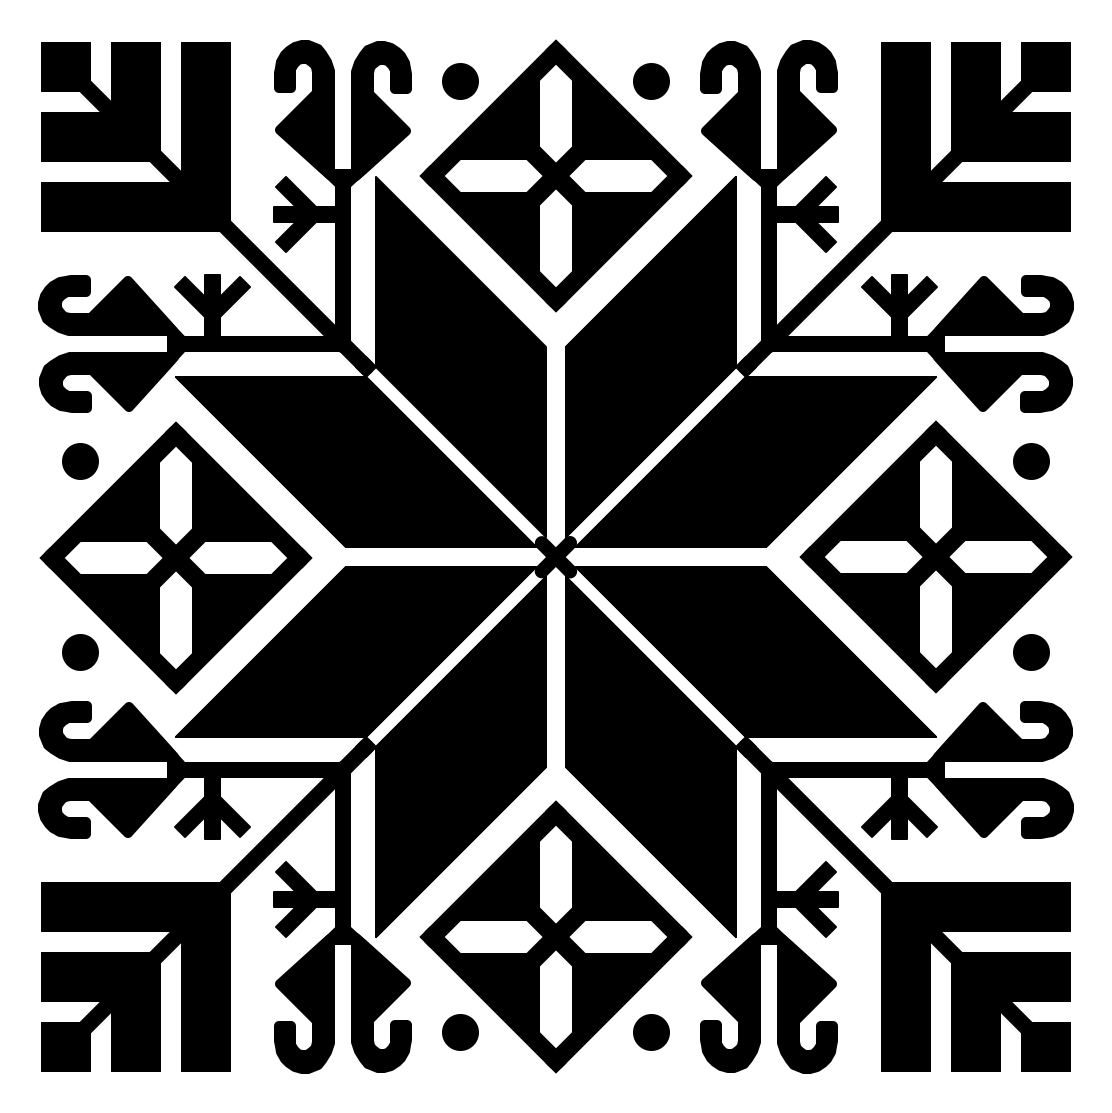
\includegraphics[scale=0.12]{__rose_black} % Черный
	\end{figure}
	\vspace*{4.0cm}
}


%\newcommand{\vepsianrose}{%
%	\begin{tikzpicture}
%		\includegraphics[scale=0.14]{vepsp}
%	\end{tikzpicture}
%}

%------------------------------------------------------------------------------------------------------------
\usetikzlibrary{celtic}
\newcommand{\uzor}{%	
\begin{center}
	\begin{tikzpicture}[%
	scale=0.17,
	transform shape,
	celtic path/.style={
		draw,
		black!10!red,
%		double distance=0.6mm,
%		line width=0.375mm
		double=white,%black!10!red, 
		double distance=0.6mm,
		line width=0.3mm
	}
	]
	\CelticDrawPath{
		size={64,4},
		max steps=64
	}
	\end{tikzpicture}	
\end{center}
}

\newcommand{\greenline}{
\begin{center}
	\begin{tikzpicture}
		\fill[fill=black!30!green,] (0,0) rectangle (10.8,0.2);
	\end{tikzpicture}
\end{center}
}
%---------------------------------------------------------------------
\usepackage{indentfirst} % Первая строка главы - с красной строки
\setlength{\parindent}{1.0cm} % Отступ слева первой абзаца
\setlength{\parskip}{0.25cm} % Отступ между абзацами

% Заголовки сверху и снизу каждой страницы (Headers & footers)
\usepackage{fancyhdr}
\pagestyle{fancyplain}

% Сделаем печать названия Части на левой странице
\newcommand*\parttitle{}
\let\origpart\part
\renewcommand*{\part}[2][]{%
	\ifx\\#1\\% optional argument not present?
	\origpart{#2}%
	\renewcommand*\parttitle{Часть \thepart.\ #2}%
	\else
	\origpart[#1]{#2}%
	\renewcommand*\parttitle{#1}%
	\fi
}

\renewcommand{\footrulewidth}{0.4pt}
%\renewcommand{\chaptermark}[1]{\markright{Часть \thepart.\ \chaptername\ \thechapter.\ #1}{}}
\renewcommand{\chaptermark}[1]{\markright{\chaptername\ \thechapter.\ #1}{}}

\fancyhead[LE]{\fancyplain{}{\bfseries \parttitle}}
\fancyhead[CE]{\fancyplain{}{}}
\fancyhead[RE]{\fancyplain{}{}}

\fancyhead[LO]{\fancyplain{}{}}
\fancyhead[CO]{\fancyplain{}{}}
\fancyhead[RO]{\fancyplain{}{\bfseries \rightmark}}
%\fancyhead[RO]{\fancyplain{}{\bfseries \chaptermark}}

\fancyfoot[LE]{\fancyplain{}{\bfseries \thepage}}
\fancyfoot[CE]{\fancyplain{}{}}
\fancyfoot[RE]{\fancyplain{}{\bfseries\scriptsize \MyVarBookName}}

\fancyfoot[LO]{\fancyplain{}{\bfseries\scriptsize \MyVarAuthorName }}
\fancyfoot[CO]{\fancyplain{}{}}
\fancyfoot[RO]{\fancyplain{}{\bfseries \thepage}}

%\renewcommand{\footrulewidth}{0.4pt}
%%\renewcommand{\chaptermark}[1]{\markright{Часть \thepart.\ \chaptername\ \thechapter.\ #1}{}}
%\renewcommand{\chaptermark}[1]{\markright{\chaptername\ \thechapter.\ #1}{}}

% Пустая страница
\newcommand\blankpage{%
	\null%
	\thispagestyle{empty}%
	\newpage%
}%

\newcommand{\sdash}{\nobreakdash-}  % Дефис неразрывный без пробелов до и после
\newcommand{\ndash}{\nobreakdash~--~}  % Короткое тире неразрывное с пробелами до и после
\newcommand{\mdash}{\nobreakdash~---~} % Длинное тире неразрывное с пробелами до и после
\newcommand{\nbdash}{\nobreakdash--}  % Короткое тире неразрывное с пробелами до и после
\newcommand{\mbdash}{\nobreakdash---} % Длинное тире неразрывное без пробелов до и после
%\newcommand{\diagdash}{\hspace*{\parindent}\nobreakdash---\thickspace}  % Короткое тире неразрывное с пробелами до и после
\newcommand{\diagdash}{\nobreakdash---\thickspace}  % Короткое тире неразрывное с пробелами до и после
%%%%%%%%%%%%%%%%%%%%%%%%%%%%%%%%%%%%%
\usepackage{tocloft,calc}
%\usepackage[newparttoc]{titlesec}
%\usepackage{titletoc}
%\usepackage{lipsum}
%\usepackage{tocbasic}
%
%\titleformat{\part}[display]
%{\centering\Huge\bfseries}{\partname~\thepart}
%{1em}{\normalfont\bfseries}
%
%\titlecontents{part}[3pc]{\addvspace{3pc}\filcenter}
%{\bfseries\partname~\thecontentslabel\\*[.2pc]\large}
%{\bfseries\large}{}[\addvspace{1pc}]
%
%%\renewcommand\cftchapdotsep{\cftdotsep}
%\titlecontents{chapter}[0em]{}
%{\bfseries\chaptername~\thecontentslabel\hspace{2em}}
%{\bfseries}
%{\mdseries\titlerule*[0.75em]{.}\bfseries\contentspage}

%\renewcommand{\cftpartfont}{\hfill\Large\bfseries\centering}
\usepackage{xpatch}
\makeatletter
\patchcmd{\l@part}{#1}{{\underline{Часть #1}}\vspace{1.5em}}{}{}
\makeatother
\addtocontents{toc}{\cftpagenumbersoff{part}}

%\renewcommand{\cftpartpresnum}{\Large Часть }
%\setlength{\cftbeforepartskip}{2.5em}
%\AtBeginDocument{\addtolength\cftpartnumwidth{\widthof{\bfseries Часть }}}

%\renewcommand{\cftchappresnum}{ ~~Глава }
\renewcommand{\cftchappresnum}{Глава~}
\setlength{\cftbeforechapskip}{0.7em}
\renewcommand\cftchapafterpnum{\vskip 0em} % for spacing after each entry
%\AtBeginDocument{\addtolength\cftchapnumwidth{\widthof{\bfseries ~~Глава~~ }}}
\AtBeginDocument{\addtolength\cftchapnumwidth{\widthof{\bfseries Глава~~}}}

\renewcommand\cftchapdotsep{\cftdotsep} % Добавление точечек к элементу chapter							
%%%%%%%%%%%%%%%%%%%%%%%%%%%%%%%%%%%%%
% Шрифт главы и секции
%\usepackage{titlesec}
%\titleformat{\chapter}[display]
%{\fontspec{NorseRus}\huge}
%{\chaptertitlename\ \thechapter}{20pt}{\Huge}
%\titleformat{\section}
%{\fontspec{NorseRus}\Large}
%{\thesection}{1em}{}
%%%%%%%%%%%%%%%%%%%%%%%%%%%%%%%%%%%%%
% Фон
\backgroundsetup{
	scale=0.75,
	color=black,
	opacity=0.5,
	angle=-1,
	contents={%
%		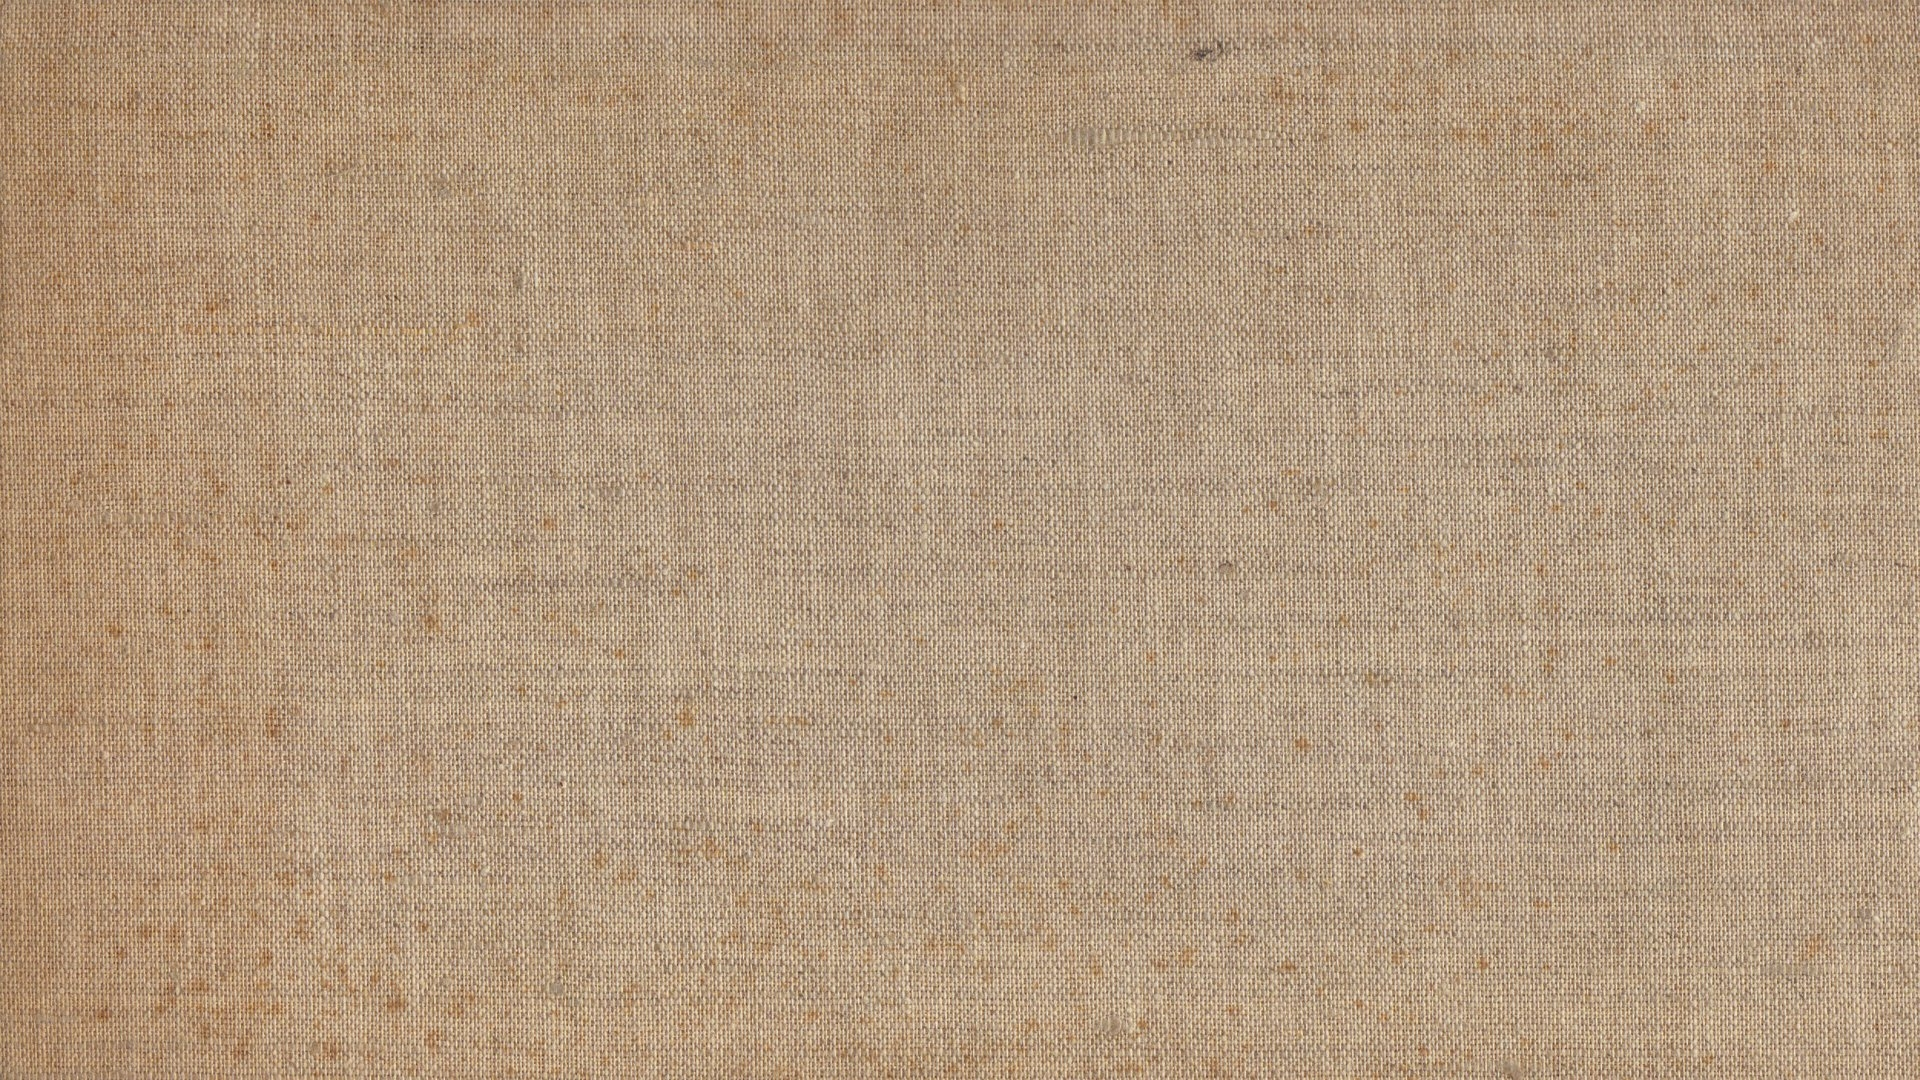
\includegraphics[width=\paperwidth,height=\paperheight]{len}
		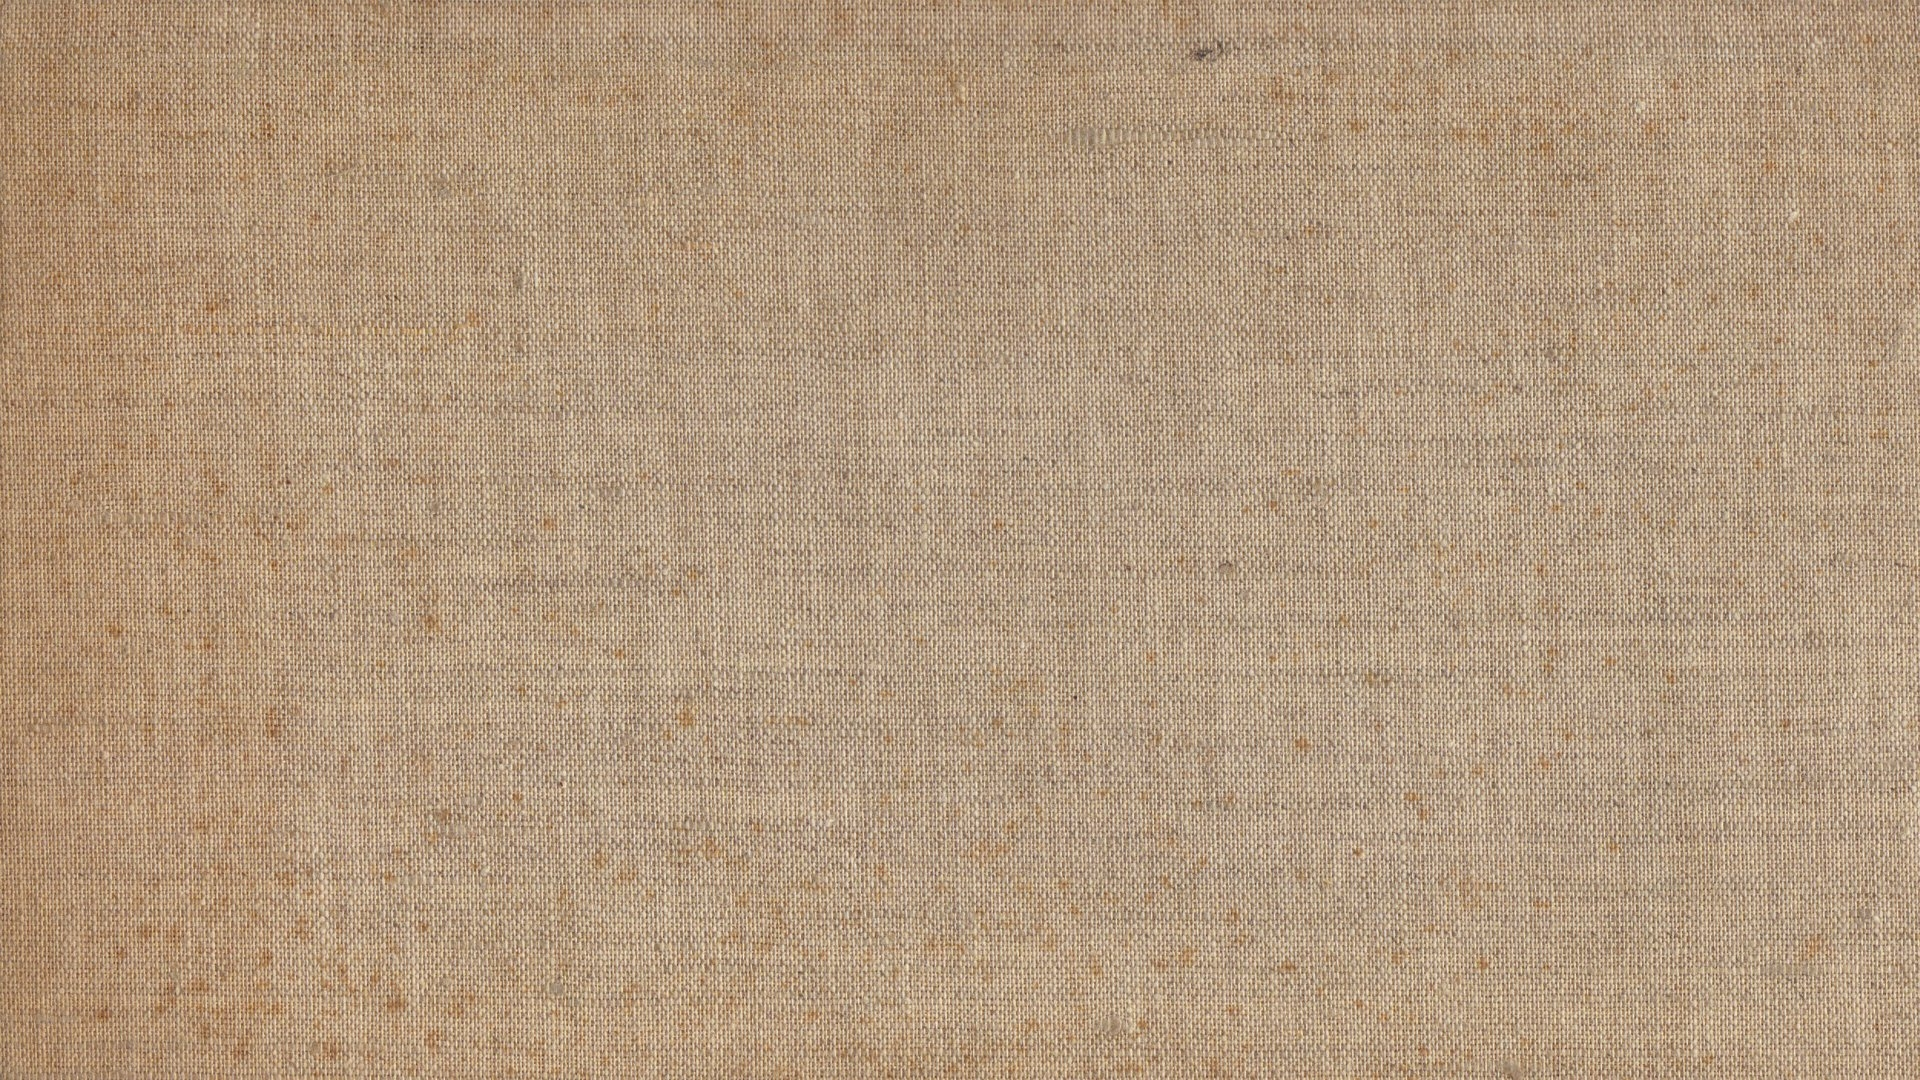
\includegraphics{len}
	}%
}
%%%%%%%%%%%%%%%%%%%%%%%%%%%%%%%%%%%%%
%\def\wordattachment{Приложение}
%
%\def\writeattachmentnonum#1#2#3{
%	\refstepcounter{attachment}
%	\hfill{\MakeUppercase{\wordattachment}}\vspace{-3mm} \\
%	\null\hfill{#1}\vspace{3mm} \\
%	{
%%		\attachmentsize\centering\MakeUppercase{#2}\par
%		\normalsize\centering\MakeUppercase{#2}\par
%	}
%	\addcontentsline{toc}{attachment}{\wordattachment.~#2}
%	\ifx&#3&\else
%	\label{#3}
%	\fi
%}
%%%%%%%%%%%%%%%%%%%%%%%%%%%%%%%%%%%%%%%%%%%%%%%%%%%%%%%%%%%%%%%%%%%%%%%%%%%%%%%%%
%% Вставляет приложение
%% \attachment{description}{title}[label]
%\def\attachment#1#2{
%	\@ifnextchar[
%	{\attachment@i{#1}{#2}}
%	{\attachment@i{#1}{#2}[]}
%}
%
%\def\attachment@i#1#2[#3]{
%	\newpage
%%	\ifnum\getnum{lastattachment}=1
%	\writeattachmentnonum{#1}{#2}{#3}
%%	\else
%%	\writeattachmentnum{#1}{#2}{#3}
%%	\fi
%}
%\usepackage{titlesec}
%\renewcommand{\thesection}{\Asbuk{section}}
%\newcommand{\intro}[1]{
%	\stepcounter{section}
%	\section*{\hfillПРИЛОЖЕНИЕ \arabic{section}}
%	\begin{center}
%		\bf{#1}
%	\end{center}
%%	\markboth{\MakeUppercase{#1}}{}
%%	\addcontentsline{toc}{chapter}{Приложение \arabic{section}. #1}
%}

\renewcommand{\thefootnote}{\fnsymbol{footnote}}
%\usepackage{parskip}

\usepackage{titlesec}
\usepackage[colorlinks=true,linktoc=all]{hyperref} % hyperfootnotes=false - не выделять сноски
\hypersetup{
	bookmarksnumbered
}
\usepackage{bookmark}
\usepackage{tcolorbox} \newcommand{\ciao}[1]{{\setlength\fboxrule{0pt}\fbox{\tcbox[colframe=black,colback=white,shrink tight,boxrule=0.5pt,extrude by=1mm]{\small #1}}}}

\usepackage{wrapfig}
\usepackage{ragged2e}
\usepackage{enumitem}

\makeatletter
\@addtoreset{chapter}{part} % Нумерация глав заново в пределах части
\makeatother  

\def\year{2025}

\usepackage{xspace} 
%\newcommand{\exldots}{!\kern0.166em.\kern0.166em.}
%\newcommand{\quldots}{?\kern0.166em.\kern0.166em.}
%\newcommand{\exldots}{\mathpunct{! \ldotp\ldotp}\xspace}  % !..
\newcommand{\exldots}{\unskip!\kern2pt\ldotp\ldotp\xspace}
\newcommand{\exldotsit}{\unskip\textit!\kern2pt\ldotp\ldotp\xspace}
\newcommand{\quldots}{\mathpunct{?\ldotp\ldotp}\xspace}  % ?..


%%%%%%%%%%%%%%%%%%%%%%%%%%%%%%%%%%%%%
\begin{document}
%%%%%%%%%%%%%%%%%%%%%%%%%%%%%%%%%%%%%%%%%%%%%%%%%%%%%%%%%%%%%%%%%%%%%%%%%%%%%%%%
%
% Координаты стоянок
%
%%%%%%%%%%%%%%%%%%%%%%%%%%%%%%%%%%%%%%%%%%%%%%%%%%%%%%%%%%%%%%%%%%%%%%%%%%%%%%%%
%
\newcommand\CoordsSunaTwentythreeStapel{${N~62.19628\degree~E~33.27931\degree}$} % Стапель 2023 г.
\newcommand\CoordsSunaTwentythreeChanelToSyargozero{${N~62.21071\degree~E~33.19865\degree}$} % Начало канала из Вендюрского в Сяргозеро 2023 г.
\newcommand\CoordsSunaTwentythreeSyargozero{${N~62.20908\degree~E~33.19042\degree}$} % Стояночное место на Сяргозере 2023 г.
\newcommand\CoordsSunaTwentythreeChanelToKulapdegi{${N~62.22188\degree~E~33.16905\degree}$} % Начало канала из Вендюрского в Сяргозеро 2023 г.
\newcommand\CoordsSunaTwentythreeSyapchozeroStoyanka{${N~62.25478\degree~E~33.12406\degree}$} % Стоянка в Сяпчозере 2023 г.
\newcommand\CoordsSunaTwentythreeChanelToToros{${N~62.27651\degree~E~33.10007\degree}$} % Начало канала из Сяпчозере в Торос 2023 г.
\newcommand\CoordsSunaTwentythreeChanelToMyaranduksa{${N~62.29707\degree~E~33.12576\degree}$} % Начало канала из Тороса в Мярандуксу 2023 г.
\newcommand\CoordsSunaTwentythreeMyaranduksaStoyanka{${N~62.32181\degree~E~33.10705\degree}$} % Стоянка в Мярандукса 2023 г.
\newcommand\CoordsSunaTwentythreeChanelToNurmis{${N~62.35101\degree~E~33.13148\degree}$} % Начало канала из Мярандуксы в Торос 2023 г.
\newcommand\CoordsSunaTwentythreeNurmisPodMostom{${N~62.39495\degree~E~33.15835\degree}$} % Проводка под мостом
\newcommand\CoordsSunaTwentythreeNurmisMesto{${N~62.40339\degree~E~33.15927\degree}$} % Стояночное место на Нурмисе
\newcommand\CoordsSunaTwentythreeNurmisRibackaya{${N~62.42979\degree~E~33.16616\degree}$} % Рыбацкая стоянка на Нурмисе
\newcommand\CoordsSunaTwentythreeChanelToLindozero{${N~62.43235\degree~E~33.16645\degree}$} % Начало канала из Нурмиса в Линдозеро 2023 г.
\newcommand\CoordsSunaTwentythreeStoyankaLittleOstrovLindozero{${N~62.44185\degree~E~33.18815\degree}$} % Стоянка на Линдозере маленький остров 2023 г.
\newcommand\CoordsSunaTwentythreeStoyankaNaMusuLindozero{${N~62.44697\degree~E~33.18316\degree}$} % Стоянка на Линдозере на западном мысу 2023 г.
\newcommand\CoordsSunaTwentythreeStoyankaPopularLindozero{${N~62.44850\degree~E~33.19657\degree}$} % Стоянка на Линдозере самая кошерная 2023 г.
\newcommand\CoordsSunaTwentythreeStoyankaNashaLindozero{${N~62.44622\degree~E~33.18984\degree}$} % Стоянка на Линдозере 2023 г.
\newcommand\CoordsSunaTwentythreeStoyankaLindozeroIstok{${N~62.44907\degree~E~33.22047\degree}$} % Стоянка на Линдозере у истока Суны
\newcommand\CoordsSunaTwentythreeMostAfterLindozero{${N~62.43843\degree~E~33.26062\degree}$} % Мост после Линдозера
\newcommand\CoordsSunaTwentythreeStoyankaBeforeSecondNoName{${N~62.45662\degree~E~33.30827\degree}$} % Стояночное место перед 2-м безымянным порогом
\newcommand\CoordsSunaTwentythreeStoyankaAfterSuhoi{${N~62.46406\degree~E~33.41163\degree}$} % Стояночное место после порога Сухой
\newcommand\CoordsSunaTwentythreeStoyankaCheranga{${N~62.46466\degree~E~33.43369\degree}$} % Стоянка в устье Черанги 2023 г.
\newcommand\CoordsSunaTwentythreeStoyankaAfterLong{${N~62.47752\degree~E~33.46658\degree}$} % Стояночное место после Длинного 2023 г.
\newcommand\CoordsSunaTwentythreeStoyankaAfterRuozmikoski{${N~62.49441\degree~E~33.46945\degree}$} % Стояночное место после Руозмикоски 2023 г.
\newcommand\CoordsSunaTwentythreeStoyankaNaSkale{${N~62.50372\degree~E~33.47823\degree}$} % Стояночное место на скале 2023 г.
\newcommand\CoordsSunaTwentythreeStoyankaPoslePorogovOne{${N~62.50837\degree~E~33.50584\degree}$} % Стояночное место 1 2023 г.
\newcommand\CoordsSunaTwentythreeStoyankaPoslePorogovTwo{${N~62.51036\degree~E~33.51539\degree}$} % Стояночное место 2 2023 г.
\newcommand\CoordsSunaTwentythreeStoyankaPoslePorogovThree{${N~62.51222\degree~E~33.55073\degree}$} % Стояночное место 3 2023 г.
\newcommand\CoordsSunaTwentythreeStoyankaPoslePorogovNaMusu{${N~62.51672\degree~E~33.55306\degree}$} % Стояночное место 4 2023 г.
\newcommand\CoordsSunaTwentythreeStoyankaPoslePorogovHoroshaya{${N~62.50820\degree~E~33.57479\degree}$} % Стояночное место 5 2023 г.
\newcommand\CoordsSunaTwentythreeStoyankaPoslePorogovNaprotiv{${N~62.50646\degree~E~33.58185\degree}$} % Стояночное место 6 2023 г.
\newcommand\CoordsSunaTwentythreeStoyankaPoslePorogovDnevka{${N~62.50643\degree~E~33.57854\degree}$} % Dnevka 2023 г.
\newcommand\CoordsSunaTwentythreeStoyankaNaRazlive{${N~62.49758\degree~E~33.58353\degree}$} % Ozero 2023 г.
\newcommand\CoordsSunaTwentythreeStoyankaKoykari{${N~62.46094\degree~E~33.59948\degree}$} % Koykari 2023 г.
\newcommand\CoordsSunaTwentythreeAntistapelGirvas{${N~62.45562\degree~E~33.66900\degree}$} % Girvas 2023 г.
%%%%%%%%%%%%%%%%%%%%%%%%%%%%%%%%%%%%%%%%%%%%%%%%%%%%%%%%%%%%%%%%%%%%%%%%%%%%%%%%
%
% Пороги
%
%%%%%%%%%%%%%%%%%%%%%%%%%%%%%%%%%%%%%%%%%%%%%%%%%%%%%%%%%%%%%%%%%%%%%%%%%%%%%%%%
\newcommand\CoordsSunaTwentythreePorogNurmisUzkiy{${N~62.41450\degree~E~33.15873\degree}$} % Узкий порог на Нурмисе
\newcommand\CoordsSunaTwentythreePorogNurmisZheskiy{${N~62.42111\degree~E~33.16003\degree}$} % Жесткий порог на Нурмисе
\newcommand\CoordsSunaTwentythreePorogUjtuzhenkoski{${N~62.43845\degree~E~33.27397\degree}$} % Уйтуженкоски
\newcommand\CoordsSunaTwentythreePorogFirstNoName{${N~62.44785\degree~E~33.29881\degree}$} % Первый безымянный которого нет
\newcommand\CoordsSunaTwentythreePorogSecondNoName{${N~62.45594\degree~E~33.31094\degree}$} % Второй безымянный
\newcommand\CoordsSunaTwentythreePorogShilmyatoykoski{${N~62.45287\degree~E~33.32570\degree}$} % Шильмятойкоски
\newcommand\CoordsSunaTwentythreePorogKovelanlietekoski{${N~62.45644\degree~E~33.33202\degree}$} % Ковеланлиентекоски
\newcommand\CoordsSunaTwentythreePorogLepolisu{${N~62.46326\degree~E~33.34190\degree}$} % Леполису
\newcommand\CoordsSunaTwentythreePorogThirdNoName{${N~62.46673\degree~E~33.35461\degree}$} % Третий безымянный в две ступени
\newcommand\CoordsSunaTwentythreePorogForthNoName{${N~62.46772\degree~E~33.36753\degree}$} % Четвертый безымянный
\newcommand\CoordsSunaTwentythreePorogSuhoi{${N~62.46002\degree~E~33.38233\degree}$} % Сухой
\newcommand\CoordsSunaTwentythreePorogKadanloamaFirstSt{${N~62.46151\degree~E~33.42405\degree}$} % Каданлоама 1 ст.
\newcommand\CoordsSunaTwentythreePorogKadanloamaSecondSt{${N~62.46347\degree~E~33.43119\degree}$} % Каданлоама 2 ст.
\newcommand\CoordsSunaTwentythreePorogDlinniyFirstSt{${N~62.46806\degree~E~33.43715\degree}$} % Длинный 1 ст.
\newcommand\CoordsSunaTwentythreePorogDlinniySecondSt{${N~62.46971\degree~E~33.45317\degree}$} % Длинный 2 ст.
\newcommand\CoordsSunaTwentythreePorogKorbikoski{${N~62.47997\degree~E~33.47025\degree}$} % Корбикоски
\newcommand\CoordsSunaTwentythreePorogRuozmikoskiFirstSt{${N~62.49472\degree~E~33.46022\degree}$} % Руозмикоски 1 ст.
\newcommand\CoordsSunaTwentythreePorogRuozmikoskiSecondSt{${N~62.49305\degree~E~33.46925\degree}$} % Руозмикоски 2 ст.
\newcommand\CoordsSunaTwentythreePorogLedyanoy{${N~62.50000\degree~E~33.46990\degree}$} % Ледяной

\relpenalty=10000
\binoppenalty=10000
\clubpenalty=10000  % Это костыль против
\widowpenalty=10000 % "висячих" строк
\righthyphenmin=200 % Избавляемся
%\interfootnotelinepenalty=10000
{\sloppy	        % от переносов слов
%%\BgThispage % Фон
\begin{titlepage}
	\newpage
	\begin{center}
		\Large \textbf \MyVarAuthorName
	\end{center}	
%	\vspace{1.75cm}	
	\vspace{0.75cm}	
	%
	%\greenline
%	\uzor
	\begin{center}
%	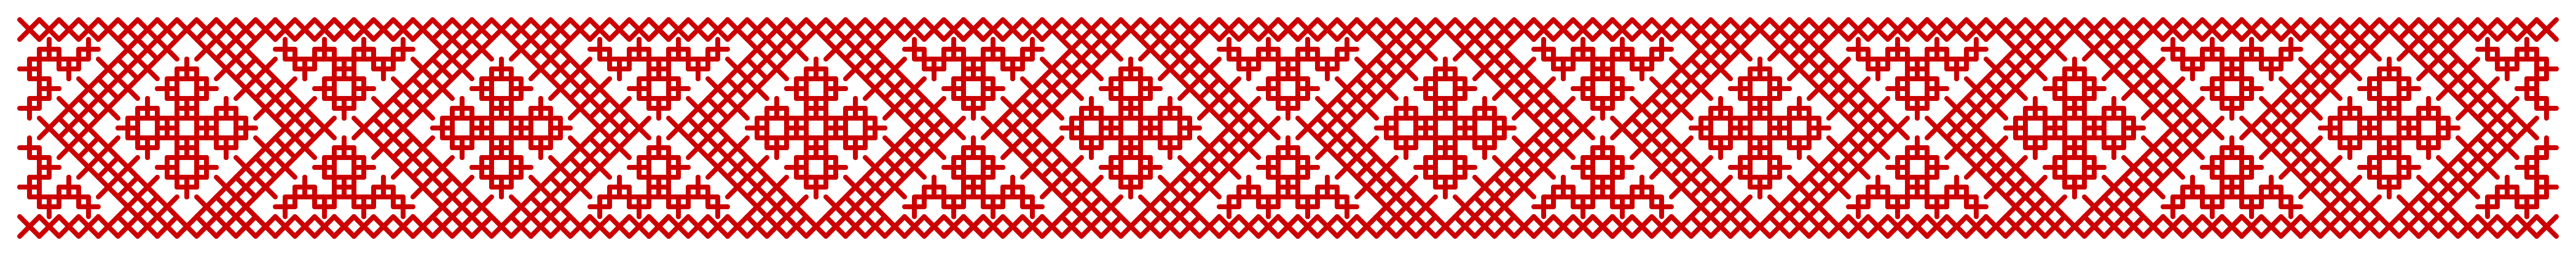
\includegraphics[scale=0.08]{vepsdr}
	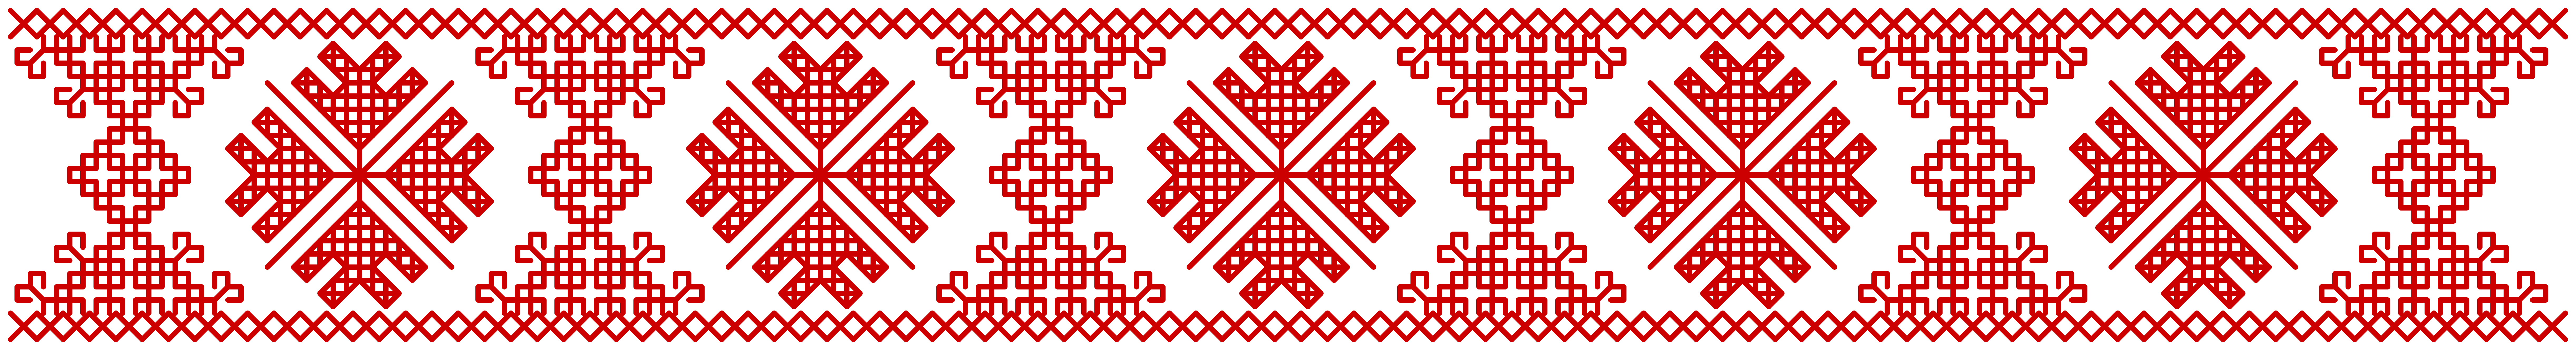
\includegraphics[scale=0.042]{karjala2}%{vepsdr6}
	\end{center}	
	%
	\begin{center}
		\Huge{\addfontfeature{LetterSpace=32.0}{КАРЕЛЬСКИЙ\\\addfontfeature{LetterSpace=83.0}ДНЕВНИК}}
	\end{center}	
%
%	\greenline
%	\uzor
	\begin{center}
%	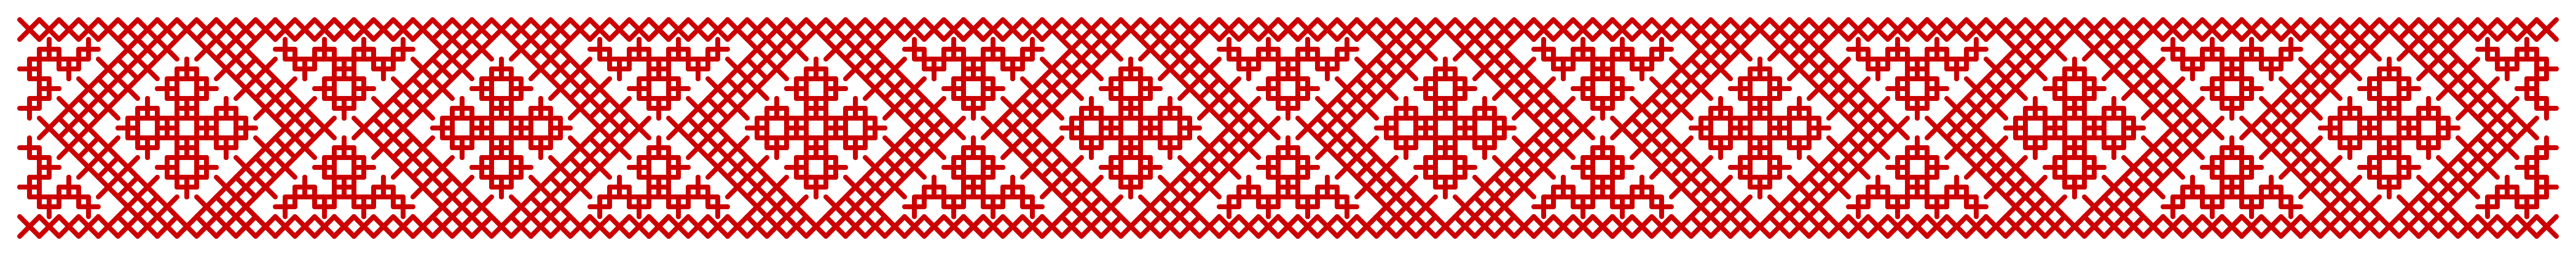
\includegraphics[scale=0.08]{vepsdr}
	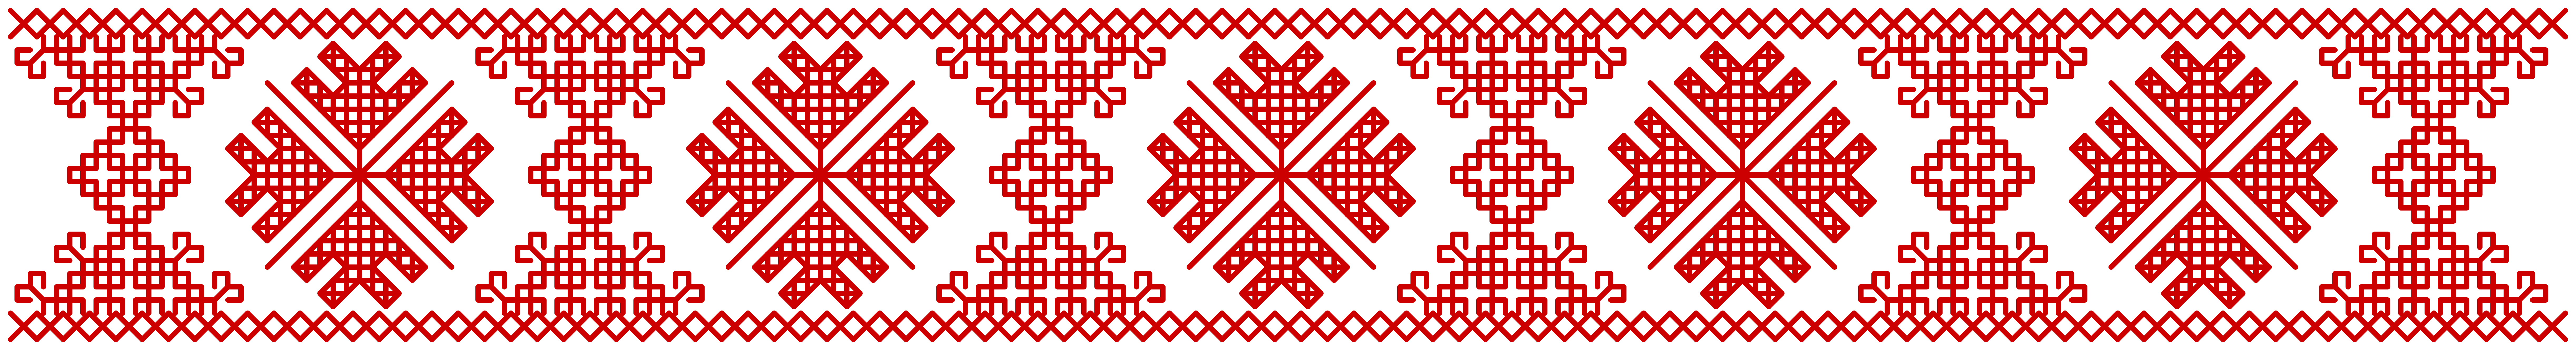
\includegraphics[scale=0.042]{karjala2}%{vepsdr6}
	\end{center}
%
	\begin{center}
		\footnotesize
%		\small 
%		\normalsize
%		{\addfontfeature{LetterSpace=12.0}
%		СБОРНИК ПОВЕСТЕЙ О СПЛАВАХ НА БАЙДАРКЕ}
%	
%		{\addfontfeature{LetterSpace=2.4}
%		ПО~РЕКАМ ГОРЮН, ЛИДЬ, ЧАГОДА, ЧАГОДОЩА, ПЕСЬ}		
		{\addfontfeature{LetterSpace=30.0}
		\textbf{ПОВЕСТЬ~~О~~СПЛАВЕ~~НА~~БАЙДАРКАХ}}
		
		{\addfontfeature{LetterSpace=28.0}
		\textbf{ПО~~МАРШРУТУ~~<<СУНСКАЯ~~ЦЕПОЧКА>>}}		
	\end{center}
%
%	\greenline
%	\uzor
%	\begin{center}
%	\includegraphics[scale=0.08]{veps}
%	\end{center}
	%	
%	\vspace{\fill}	
%	\begin{center}
%		\small\textbf{
%		Москва \linebreak 
%		2022 \linebreak
%		Самиздат}
%	\end{center}
	\vspace{\fill}	
	\begin{center}\normalsize Москва\end{center}
	\vspace{-1.1cm}
	\begin{center}
\includegraphics[scale=0.13]{maska}\end{center}
	\vspace{-1.24cm}
	\begin{center}\normalsize 2023\end{center}	
\end{titlepage}   % Обложка
%%\chapter*{}
%\newpage
{
\thispagestyle{empty}
%
\small{
\begin{flushleft}
\textbf{%
	УДК \UDK \\
	ББК \BBK \\
	\BibCode \\
}
\end{flushleft}
%
%\vspace{3cm}
\vspace{1cm}
%
\begin{flushright}
{
\begin{tabular}[c]{>{\raggedright}m{14mm} >{\raggedright}m{95mm} }
	\textbf{\BibCode} & \MyVarAuthorName \tabularnewline
	~ & \MyVarBookName \tabularnewline
	~ & \MyVarBookNamesec \tabularnewline
	~ & М.:~ООО~<<ИПЦ~"`Маска"'>>,~\year\mdash \pageref{LastPage} c. \tabularnewline	
	~ & \textbf{\ISBN} \tabularnewline
	~ & \ciao{16+}
\end{tabular}
}
\end{flushright}
%
%\vspace{3.0cm}%\vspace{4.0cm}
\vspace{0.5cm}
\hspace{1.0cm} В повести рассказывается о байдарочном сплаве в~Карелии по маршруту <<Сунская цепочка>>\cite{Шилов}, а также о событиях, предшествующих этому походу. Своеобразный <<кольцевой>> маршрут, замкнутый на посёлок Гирвас, состоит из двух частей: в первой путешественники побывают на череде озёр и небольших речушек, а~во~второй, начинающейся с~Линдозера, предстоит штурм 14 порогов 2~категории сложности. Цепочка сменяющих друг друга рек и озёр приносит сплавщикам массу впечатлений, приправленных переменчивой карельской погодой, а~также местными ягодами, грибами и, конечно же, свежевыловленной рыбой. При заброске путешественники осмотрят крепость в~Старой Ладоге, побывают на водопаде Кивач, а~при~выброске\mdash на~палеовулкане Гирвас.

\vspace{4mm}
\noindent \underline{Ключевые слова}: водный туризм, речной сплав, туристкий поход, байдарочный поход, Карелия, путевые заметки, дневник похода.
%
%\begin{flushright}
%\textbf{%
%	УДК \UDK \\
%	ББК \BBK \\
%	\BibCode \\
%}
%\end{flushright}
%
%\vspace{\fill}
\vspace{4mm}
%\vspace{1.0cm}
%

\noindent\makebox[\textwidth][s]{\textbf{\ISBN}\hfill{\copyright~\MyVarAuthorName,~\year}}
}

%{
%\begin{longtable}[c]{>{\raggedright}m{56mm} >{\raggedleft}m{56mm} }
%	\textbf{\ISBN} & {\copyright~\MyVarAuthorName,~\year} \tabularnewline
%\end{longtable}
%}
}
%%\chapter*{}

\clearpage               % переход на новую страницу
\thispagestyle{plain}   % или 'empty', если не нужен номер страницы
% Без \chapter, \section и т.п.

\noindent{\textbf{\large{<<Карельский дневник>>, Соболев А.А.}}}

{\small%\footnotesize%
\vspace{2mm}
\setlength{\parskip}{2mm}
%\setlength{\parindent}{1em}
\setlength{\parindent}{1.0cm}
Перед вами документально-художественная проза о~водном туризме, продолжение водно-походной летописи А.А. Соболева, начатой в <<Повести о сплаве по рекам Лидь, Чагода и Чагодоща>>. Новая повесть выводит команду сплавщиков в пространство иной географии и сложности\mdash в Карелию, с её порогами, погодной неуступчивостью и~архетипической <<силой земли>>. Это не просто байдарочный дневник, это целостная хроника духовного обновления, личных кризисов, усталости от~города, быта, работы, и~попытки обрести смысл в природе, дружбе, простом труде.

\noindent{\textbf{\underline{Основная тема}}}\mdash повествование о байдарочном походе по~Карелии как метафора личного поиска и выхода из~душевного~тупика.

\noindent{\textbf{\underline{Особенности повествования:}}}
\begin{enumerate}[leftmargin=1cm, itemsep=0pt, topsep=0pt] %2.6em
%	\item[--] переплетение автобиографии и художественного текста;
	\item[--] лирические отступления, философские размышления;
	\item[--] быт и технические детали водного туризма;
	\item[--] внутренние монологи героя.
\end{enumerate}

\noindent{\textbf{\underline{Главные темы:}}}
\begin{enumerate}[leftmargin=1cm, itemsep=0pt, topsep=0pt]
	\item[--] водный байдарочный туризм;	
	\item[--] дружба и товарищество;	
	\item[--] природа как лекарство от выгорания и усталости от бытия.
%	\item[--] ностальгия и взросление;
%	\item[--] природа как лекарство для душевного равновесия.
\end{enumerate}

\noindent{\textbf{\underline{Для кого эта книга?}}}
\begin{enumerate}[leftmargin=1cm, itemsep=0pt, topsep=0pt]
	\item[--] любителей приключений и сплавов;
	\item[--] ценителей психологической прозы;
	\item[--] все, кто ищет свой маршрут\mdash внешний и внутренний.	
\end{enumerate}

\noindent{\textbf{\underline{Почему стоит прочитать?}}}
\begin{enumerate}[leftmargin=1cm, itemsep=0pt, topsep=0pt]
	\item[--] искренность и сила голоса автора;
	\item[--] атмосфера настоящего <<дикого>> похода;
	\item[--] Карелия как литературный герой.	
\end{enumerate}


%Повесть разворачивается в нескольких плоскостях: это прежде всего экзистенциальная усталость, желание сбежать, попытка обрести равновесие, плавно перетекающие в подготовку к~сплаву, сбору команды, выбору маршрута, закупкам, составлению лоций,  планов и, наконец, сам сплав как квинтэссенция желаний и помыслов команды сплавщиков. 
%
%История начинается с тоски по реке и выстраивает путь от городской удушающей рутины к речной стихии, к природной и внутренней свободе. Ярко раскрываются эпизоды подготовки: бытовые сцены, диалоги с друзьями, застолья, где читатель узнаёт каждого персонажа живо и~с~юмором.
%
%Язык повести\mdash эмоционально насыщенный, с~элементами иронии, фольклорной стилизации, современной мемной лексики и живых диалогов. Каждая глава построена \makebox[\linewidth][s]{как самостоятельный эпизод, наполненный как внутренним}

}

\clearpage               

\thispagestyle{plain}   % или 'empty', если не нужен номер страницы
%\noindent содержанием, так и внешним действием. Автор не боится говорить о тревожности и ностальгии, депрессии и смерти, что придаёт книге психологическую глубину. Карелия, как главное место действия повести, изображена как культурный и геопоэтический символ, насыщена отсылками к древней истории, культуре, архитектуре, природным достопримечательностям.
%
%<<Карельский дневник>>\mdash это не просто повесть о~байдарках, это повесть о~стремлении выжить душой в~век информационной и эмоциональной перегруженности. Это многослойное литературное произведение с внятным стилем и яркой философией.
%
%Рекомендовано: туристам\sdash водникам, урбанистам в~кризисе, ценителям путешествий и внутреннего пути. Достоинством произведения 

{\small%\footnotesize%
	

\noindent{\textbf{\underline{Жанровая специфика}}}

Повесть сочетает в себе жанровые признаки мемуарной литературы, автобиографического романа и тревел-лога. В отличие от сухого отчёта о путешествии, текст насыщен эмоциональными, психологическими и культурными наблюдениями, комментариями персонажей на происходящее в сплаве. %Это делает <<Карельский дневник>> не просто путевыми заметками, а~художественным документом эпохи.

\noindent{\textbf{\underline{Композиция}}}

Повествование построено как череда сцен и диалогов, объединённых главной идеей\mdash подготовкой и прохождением похода. Автор делает акцент на подробностях, которые в~совокупности создают эффект живого присутствия. Ритм уравновешен: бытовые, философские и походные сцены сменяют друг друга, раскрывая читателю персонажей.

\noindent{\textbf{\underline{Персонажи и образ рассказчика}}}

Центральный персонаж\mdash Шурик\mdash несёт в себе черты автора. Он\mdash ироничный, уставший, честный и рефлексирующий. Его внутренние монологи задают тон всей повести. Остальные герои\mdash Киря, Серёга, Паша и новичок в сплаве\mdash Руслан\mdash создают многоголосие команды и отражают разные варианты реакции на происходящее в походе.

\noindent{\textbf{\underline{Язык и стиль}}}

Лексика нарочито простая, насыщенная просторечием, фразеологизмами, молодёжным сленгом, туристическим жаргоном, морскими терминами. Это нисколько не~снижает художественного уровня, напротив\mdash создаёт ощущение искренности, близости читателю и добавляет аутентичности, целостности повествованию. Часто встречаются отсылки на~разнообразную литературу, что придаёт тексту культурную~плотность и налёт научной достоверности.
	
}

\clearpage

\thispagestyle{plain}   % или 'empty', если не нужен номер страницы
%\noindent содержанием, так и внешним действием. Автор не боится говорить о тревожности и ностальгии, депрессии и смерти, что придаёт книге психологическую глубину. Карелия, как главное место действия повести, изображена как культурный и геопоэтический символ, насыщена отсылками к древней истории, культуре, архитектуре, природным достопримечательностям.
%
%<<Карельский дневник>>\mdash это не просто повесть о~байдарках, это повесть о~стремлении выжить душой в~век информационной и эмоциональной перегруженности. Это многослойное литературное произведение с внятным стилем и яркой философией.
%
%Рекомендовано: туристам\sdash водникам, урбанистам в~кризисе, ценителям путешествий и внутреннего пути. Достоинством произведения 

{\small%\footnotesize%
		
\noindent{\textbf{\underline{Тематика и мотивы}}}

Ключевые темы: усталость от современности, тревожность, кризис среднего возраста, ценность мужской дружбы, стремление к аскезе и свободе. Мотив воды, дороги, преодоления и дикой природы\mdash классические элементы нарратива, где путь становится символом очищения.

\noindent{\textbf{\underline{Вывод}}}

<<Карельский дневник>>\mdash зрелая, живая и очень личная повесть. В ней одновременно чувствуется и боль, и надежда, и~самоирония, и~любовь к жизни. Текст можно рекомендовать как яркий пример современной непафосной прозы, способной тронуть и читателя\sdash походника, и обычного жителя большого города.

}

\vspace{1.0mm}

\noindent\textit{Устраивайся поудобнее, читатель, мы начинаем наш путь!}

\vspace{1.0mm}

\begin{figure}[h]
	\centering
	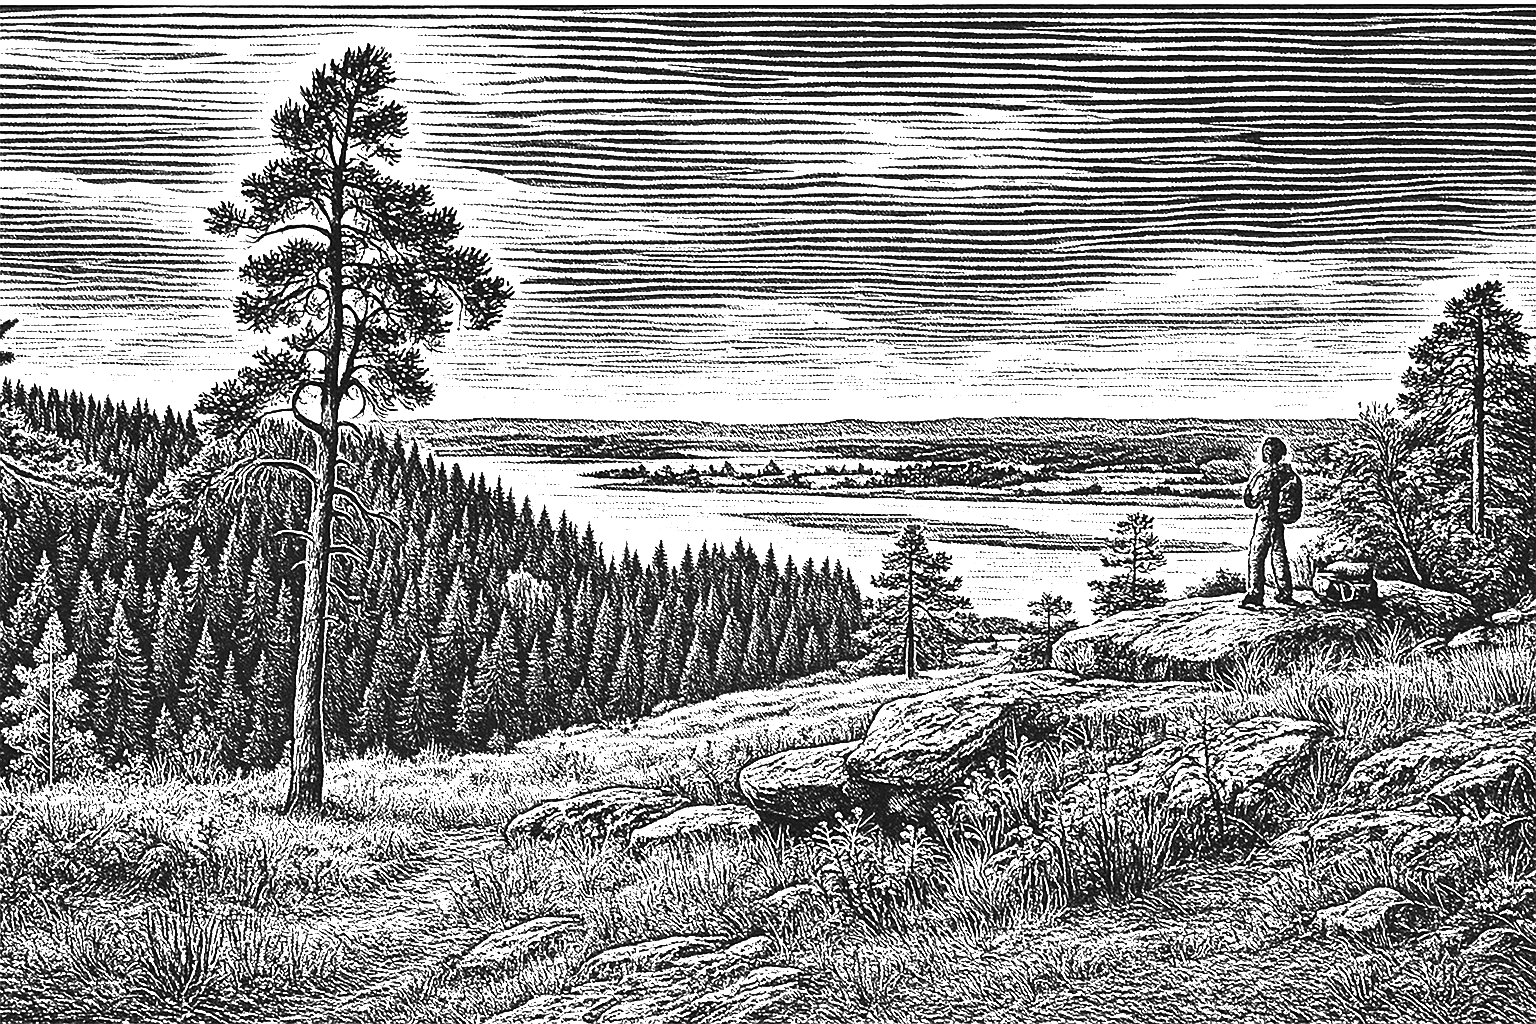
\includegraphics[width=1.0\textwidth]{00_karjala}
%	\caption{\small\textit{Устраивайся поудобнее, читатель, мы начинаем наш путь!}}
\end{figure}

\vspace{5mm}

\vspace{\fill}
%{\raggedright{\scriptsize\textit{автоматическая рецензия подготовлена ИИ}}}
\noindent
\begin{minipage}[t]{0.2\textwidth}
	\raggedright ~
\end{minipage}
\hfill
\begin{minipage}[t]{0.8\textwidth}
	\raggedleft {\scriptsize\textit{автоматическая рецензия подготовлена ИИ}}
\end{minipage}
\clearpage

%{
%\vspace{-5cm}
%<<Карельский дневник>>--- документально-художественная проза о водном туризме, продолжение водно-походной летописи А.А. Соболева, начатой в <<Повести о сплаве по рекам Лидь, Чагода и Чагодоща>>. Новая повесть выводит команду сплавщиков в пространство иной географии и сложности--- в Карелию, с её порогами, погодной неуступчивостью и архетипической <<силой земли>>. Это не просто байдарочный дневник, это целостная хроника духовного обновления, личных кризисов, усталости от города, быта, работы, и попытки обрести смысл в природе, дружбе и простом, почти первобытном труде.
%
%Повесть разворачивается в нескольких плоскостях: это прежде всего экзистенциальная усталость, желание сбежать, попытка обрести равновесие, плавно перетекающие в подготовку к сплаву, сбору команды, выбору маршрута, закупкам, составлению лоций,  планов и, наконец, сам сплав как квинтэссенция желаний и помыслов команды сплавщиков. 
%
%История начинается с тоски по реке и выстраивает путь от городской удушающей рутины к речной стихии, к природной и внутренней свободе. Ярко раскрываются эпизоды подготовки: бытовые сцены, диалоги с друзьями, застолья, где читатель узнаёт каждого персонажа живо и с юмором.
%
%Язык повести--- эмоционально насыщенный, с элементами иронии, фольклорной стилизации, современной мемной лексики и живых диалогов. Каждая глава построена как самостоятельный эпизод, наполненный как внутренним содержанием, так и внешним действием. Автор не боится говорить о тревожности, депрессии, ностальгии, смерти, что придаёт книге психологическую глубину. Карелия, как главное место действия повести, изображена как культурный и геопоэтический символ, насыщена отсылками к древней истории, культуре, архитектуре, природным достопримечательностям.
%
%<<Карельский дневник>>--- это не просто повесть о байдарках, это повесть о стремлении выжить душой в век информационной и эмоциональной перегрузки. Это многослойное литературное произведение с внятным стилем и яркой философией.
%
%Рекомендовано: туристам-водникам, урбанистам в~кризисе, ценителям путешествий и внутреннего пути.
%}


%%%% --> Хорошее
%В повести рассказывается о байдарочном сплаве в~Карелии по маршруту <<Сунская цепочка>>\cite{Шилов}, а также немного о предыстории этого похода. Своеобразный <<кольцевой>> маршрут, замкнутый на посёлок Гирвас, состоит из двух частей: в первой путешественники побывают на череде озёр и небольших речушек, а~во~второй, начинающейся с Линдозера, предстоит штурм 14 порогов 2~категории сложности. Цепочка сменяющих друг друга рек и озёр приносит сплавщикам массу впечатлений, приправленных переменчивой карельской погодой, а~также местными ягодами, грибами и, конечно же, свежевыловленной рыбой. При заброске путешественники осмотрят крепость в Старой Ладоге, побывают на водопаде Кивач, а~при~выброске\mdash на~палеовулкане Гирвас.

%%%% --> старое
%В повести рассказывается о байдарочном сплаве в~Карелии по маршруту <<Сунская цепочка>>\cite{Шилов}. Своеобразный <<кольцевой>> маршрут, замкнутый на посёлок Гирвас, состоит из двух частей: в первой путешественники побывают на череде озёр и небольших речушек, а~во~второй, начинающейся с Линдозера, предстоит штурм 14 порогов 2~категории сложности. Цепочка сменяющих друг друга рек и озёр приносит сплавщикам массу впечатлений, приправленных переменчивой карельской погодой, а~также местными ягодами, грибами и, конечно же, свежевыловленной рыбой. При заброске путешественники осмотрят крепость в Старой Ладоге, побывают на водопаде Кивач, а~при~выброске\mdash на палеовулкане Гирвас.

%\vspace{\fill}
%\begin{flushright}
%	\copyright~Соболев~А.А.~2022
%\end{flushright}
 % Аннотация глобально к сборнику
%\afterpage{\blankpage}
%\tableofcontents
% Замена \blankpage в данном случае:
%
%\newpage
%{
%\null
%\thispagestyle{empty}
%\chapter*{}
\begin{flushright}
\vspace{2.0cm}
\textit{ \large {
%Жаждущим диких походов посвящается.\\
Посвящается N.\\
\vspace{\fill}
Все имена, названия, события,\\
время и место действия вымышлены,\\
а совпадения случайны.
}}
\end{flushright}
%}
%
%\newpage
%{
%\null
%\thispagestyle{empty}
%}
%\newpage
%
%{
%%\setlength{\cftbeforetoctitleskip}{1.5cm}%чтобы влезло на 1 страницу 11 шрифт
%%\setlength{\cftbeforetoctitleskip}{0.5cm}%чтобы влезло на 1 страницу 12 шрифт
%%\setlength{\cftbeforetoctitleskip}{0.0cm}%чтобы влезло на 1 страницу 12 шрифт c прологом
%%\setlength{\cftbeforetoctitleskip}{-0.7cm}%чтобы влезло на 1 страницу 12 шрифт c прологом
%\setlength{\cftbeforetoctitleskip}{-0.9cm}%чтобы влезло на 1 страницу 12 шрифт c прологом
%\pdfbookmark[0]{\contentsname}{toc} % Добавлять перед \tableofcontents
%\tableofcontents
%}
%
% БЛАГОДАРНОСТИ 
%\cleardoublepage
\phantomsection
\thispagestyle{empty}
\addtocontents{toc}{\vspace{-10mm}}
\addcontentsline{toc}{chapter}{Благодарности}
\section*{Благодарности}
\begin{enumerate}
%\vspace{12mm}	
\itemsep0.1mm 
%\item[\ding{72}] Моим родителям\mdash без комментариев.
%
\item[\ding{72}] Моей любящей жене Екатерине, которая стала первопричиной моего увлечения водным туризмом и~идеальной спутницей не только в походах, но~и~в~жизни.
%
\item[\ding{72}] Красавину\enskip Сергею\enskip Юрьевичу\mdash моему наставнику, коллеге и~товарищу, за многолетнюю совместную работу, за поддержку, бесценные советы и~опыт, за~знакомство с миром байдарочной свободы.
%
\item[\ding{72}] Краузу\enskip Павлу\enskip Викторовичу\mdash моему коллеге и~товарищу, за ежегодное участие в наших авантюрах, абсолютную стойкость в перенесении походных условий и отличную рыбалку.
%
\item[\ding{72}] Лунёву\enskip Сергею\enskip Александровичу\mdash моему другу и~товарищу, одногруппнику по институту, за~многолетнюю дружбу и за то, что ты преодолел тогда боязнь воды.
%
\item[\ding{72}] Рябкову\enskip Кириллу\enskip Александровичу\mdash моему другу и~товарищу, за неоценимый вклад в психологический баланс в нашей группе; очень жалею, что раньше не~узнал о том, что ты тоже байдарочник!
%
\item[\ding{72}] Одегову\enskip Руслану\enskip N-овичу\mdash за решительность, оптимизм и~бесстрашие на порогах, за готовность рискнуть пойти в~свой первый сплав сразу на 2 к.с.
\end{enumerate}
%
% ПРОЛОГ
%\afterpage{\blankpage}
%{

{
\cleardoublepage
\phantomsection

%\fancyhead[LE]{\fancyplain{}{}}
%\fancyhead[RO]{\fancyplain{}{}}

\addcontentsline{toc}{chapter}{Пролог}
%\addtocontents{toc}{\vspace{0mm}}
\section*{Пролог}

\fancyhead[LE]{\fancyplain{}{}}
\fancyhead[RO]{\fancyplain{}{}}

Карелия$\ldots$ что чувствует турист\sdash водник, слыша это слово? Сердце начинает стучать чаще, разум затуманивается! Карелия, Карьяла, Karjala\mdash зовёт, манит, завлекает! Чистейшие сосновые леса на каменистых берегах, а под ногами мшаник и поля черники, голубики$\ldots$ Карелия это красивая и~строгая северная природа, скалы, исполинские янтарные сосны, пьянящий воздух, обилие ягод, грибов, рыбы, и, естественно, пороги\footnote{Каменистый участок в русле с повышенной скоростью течения и~относительно большим падением отметок уровня воды.}. Куда же без них? 

Сотни, если не тысячи, водников каждый год посещают эти заповедные места, эти порожистые речки, заставляющие неслабо напрячься на порогах капитанов и~впередсмотрящих туристких судёнышек. Но этот небольшой экстрим с~лихвой окупается всем, что окружает сплавщиков на~маршруте\mdash и~дарами леса, и чувством единения с карельской природой\mdash северной, порою суровой и~жестковатой, а порою ласковой и приветливой, отчего делается так хорошо на душе, что не передать словами; уха на свежевыловленной рыбе, шум порогов, белая пена и валы которых заставляют испытать порою животный страх и чувство преклонения перед силой стихии\mdash за этим едут сюда люди, которым опостылел город, кто хочет духовно очиститься, опустошить сознание, дать природе омыть тебя бодрящей водой и смыть городскую грязь\mdash физически и~духовно. Это место\mdash место припадения к истокам, место силы, место древа жизни. Такой представлялась Карелия. Такой она и оказалась, приняв команду сплавщиков и~тёплыми дождями, и ярким августовским солнышком, а~иногда и порывистым ветром, пробирающим до костей даже в штормовке.  

Откуда есть пошла Земля Русская? Да не скажет никто\mdash сплошное надувательство\mdash дальше нескольких сотен лет назад никто не скажет наверняка что и как там было. Считается, что Старая Ладога была местом, куда был призван княжить Рюрик (Зачем, спрашивается, призван? Своих <<рюриков>> мало было?). Впрочем тут же вам скажут, что, скорее всего, этим местом должен быть Великий Новгород и пошло поехало\mdash куча теорий. Но~все они, конечно же, не на пустом месте. Принято считать, что так называемое призвание варягов на Русь таки имело место и~Рюрик всё же сначала обосновался в Старой Ладоге. Именно поэтому команда сплавщиков решила остановиться в этом городке по пути в~Карелию, поскольку интересно и~крепость посмотреть, и ехать до Карелии от Москвы, что называется, за~1 присест\mdash очень тяжело. Посему, решили ехать с ночёвкой в Старой Ладоге, отведя утро второго дня на осмотр крепости и окрестностей. 

\renewcommand*{\thefootnote}{\fnsymbol{footnote}}
%\renewcommand*{\thefootnote}{\arabic{footnote}}
\setcounter{footnote}{0}
Отчего же вдруг они отошли от~привычного бассейна Мологи\cite{СоболевВепсскаяЛетопись}? Всё~просто\mdash наиболее интересные реки мологского бассейна были пройдены\mdash Лидь, Чагода, Чагодоща, Горюн, Песь. Хотелось чего\sdash то принципиально нового! Последнний раз команда ходила в сплав в 2019 году, о~чём даже была вырезана ножом памятная надпись на~беседке у~антистапеля\footnote{применительно к байдарочным сплавам\mdash место разборки байдарок, как правило, при окончании маршрута.}: %(да, именно такими буквами): 
%Непокорённой осталась, разве что, Кобожа, но характер берегов там как\sdash то не~способствовал склонению желания в её сторону.
%\newpage

%\vspace{-5mm}
%\vspace{-4mm}
{\centering\LARGE{\fontspec{NorseRus}{%\LARGE
			Посл.\\раз\\2019\\
}}}

\newpage
И как накаркали\mdash ситуация в мире пошла, что называется, по~наклонной. Сначала ужас и сумасшествие пандемии 2020\thinspace\nobreakdash--\thinspace 2021 года, сопровождаемое чехардой смены работ, удалёнкой, тихим схождением с ума от удалёнки и всеобщей окружающей обстановки. Потом ситуация с~вооруженным конфликтом у~наших западных границ. Всё~это, конечно~же, счастья не~добавляло абсолютно. Закрадывалась мысль\mdash а может надпись <<Посл. раз 2019>> и вправду уже стала пророческой? Но нет, рановато! Кто\sdash то там лает, а караван идёт\mdash волю к~путешествиям не~заглушишь ничем!

Шурику, предводителю, командиру команды байдарочников, вдруг вспомнились ставшие для него чем\sdash то сакральным строки из произведения <<Географ глобус пропил>>: <<\textit{Конечно, обалдели все и от меня, и от такого похода. Всем домой хочется. Половина клянётся, что больше ни~в~жисть из города не вылезет. Но всё это\mdash пустые обещания. <...> Сейчас все хотят одного: тепла, уюта, покоя. Но отрава бродяжничества уже в~крови. И~никакого покоя дома они не~обретут. Снова начнёт тревожить вечное влечение дорог\mdash едва просохнет одежда и отмоется грязь из\sdash под ногтей. Я~это знаю точно. Я~и~сам сто раз зарекался\mdash больше ни ногой. И~где~я~сейчас?}>>\cite{ГеографГлобусПропил}.

Прочитав <<Географа>> перед своим первым байдарочным сплавом, Шурик был поражён этим произведением, насколько оно легло на душу, насколько пришлось близким и понятным. Однако тогда приведённые выше строки не~вспыхивали так ярким пламенем, безумным пожаром, как сейчас\mdash разве мог он тогда, в 2015 году зарекаться, что, мол, ни ногой больше? А~в~2019 вдруг с~горечью вырезает <<Посл. раз>>. И вот, в 2023 Шурик снова сидит поздним вечером у себя на кухне, разложив на~столе святая святых\mdash топокарту маршрута и волнительно прикидывает места стоянок, стратегию прохождения маршрута и штурм порогов$\ldots$ 

Одно верно\mdash отрава бродяжничества в крови и этого не отнять\mdash поход 2023 года только подтвердил это. Стоит только позволить себе мимолётную слабость\mdash на 1 секунду закрыть глаза и подумать: <<Вот щ\sdash щ\sdash щас бы на реку$\ldots$>> и~всё, ты уже испытываешь то самое сладкое и~томительное \textit{<<вечное влечение дорог>>}$\ldots$

\begin{center}
	\psvectorian[scale=0.4]{88} % Красивый вензелёк :)
\end{center}

%\vspace{5mm}

%\begin{flushright}
%	\textit{Соболев А.А., 2023 г.}
%	%\copyright~Соболев~А.А.,~Москва,~27.08.2015
%\end{flushright}

}

}

%\afterpage{\blankpage}
%
%\chapter{Тест}

Тестовая глава для печати всех иллюстраций.

\newpage

%----------------------------------------------------------------
% 1 ГЛАВА
%----------------------------------------------------------------


\begin{figure}[h]
\centering
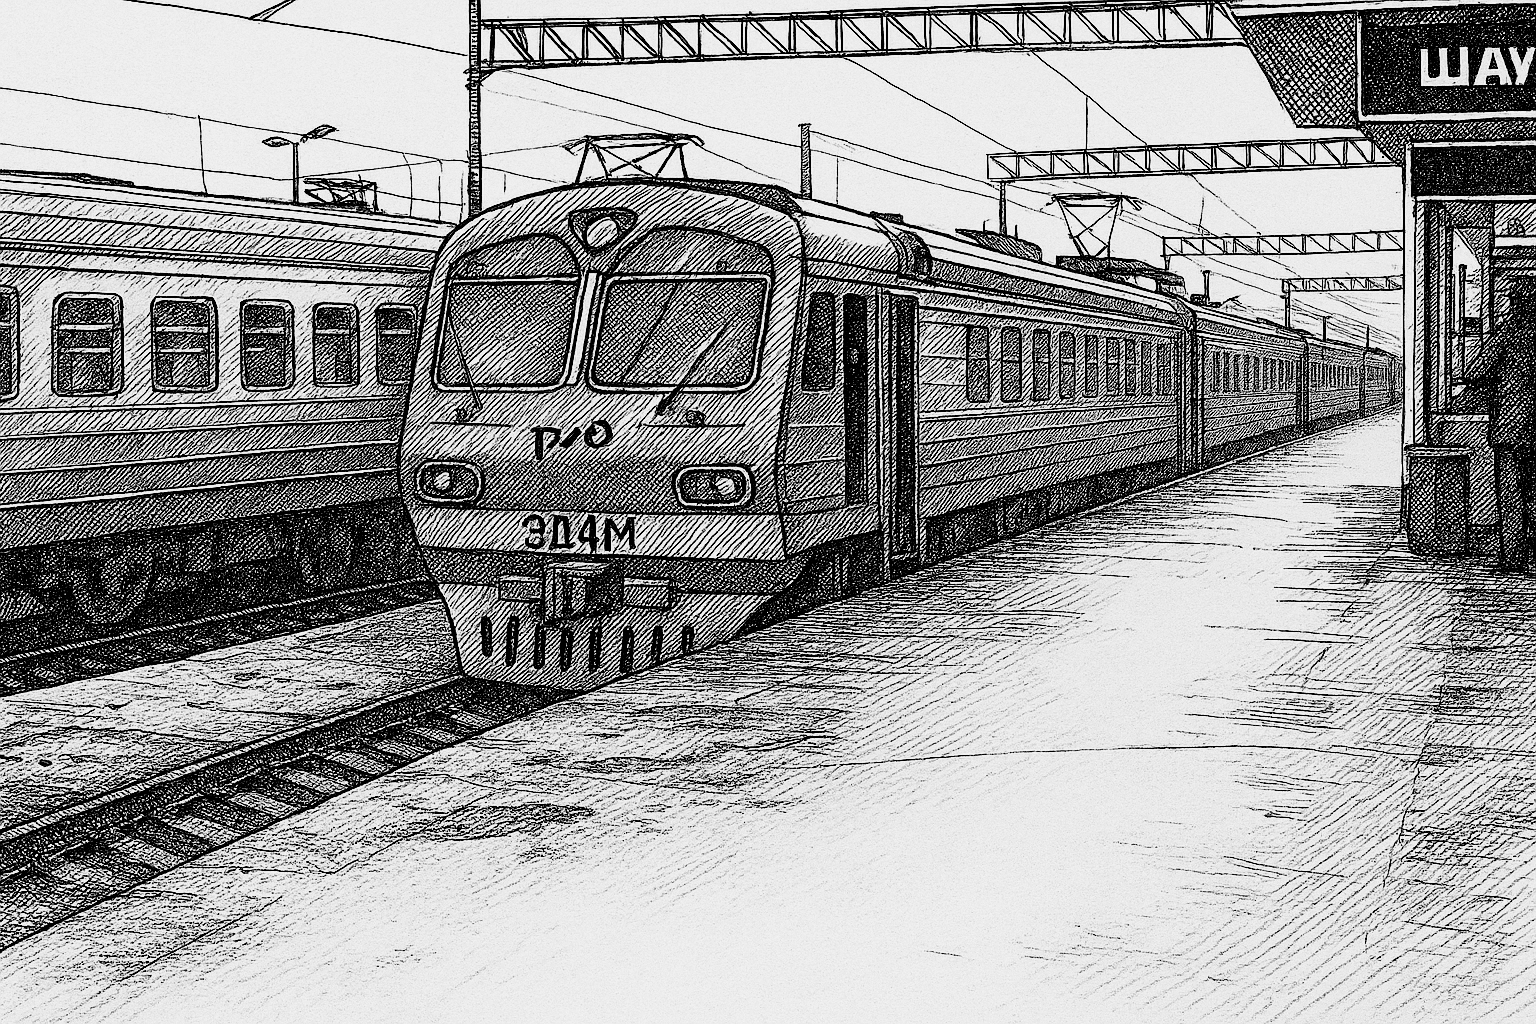
\includegraphics[width=1.0\textwidth]{01_train}
\caption{\small\textit{...в электричке c Курского вокзала...}}	
\end{figure}

%----------------------------------------------------------------
% 2 ГЛАВА
%----------------------------------------------------------------

\newpage

Сеструха, тем временем, задорно отплясывала в центре зала, широко улыбаясь, светя забитой татухой рукой и~оголёнными плечами, справедливо упиваясь торжеством молодости, красоты, задора. Светлые завитые локоны подплясывали в такт движениям, вишнёвое вечернее платье подчёркивало все её сочные достоинства.

\noindent
\begin{minipage}{0.48\textwidth}
	\setlength{\parindent}{1.0cm}  % Включаем красную строку
	
	\indent \diagdash Пошли~потанцуем?\mdash вдруг жарко шепнула жена на~ухо Шурику.
	
	\indent \diagdash А пошли!\mdash он приобнял жену и закружил в толпе танцующих гостей, словно желая выкружить все крамольные мысли из~головы$\ldots$
	
	\indent $\ldots$Стол ломился, друзья широко, разгульно праздновали:
	
	\indent \diagdash Дорогие Кирилл и~Надежда$\ldots$\mdash полились речи, всё как обычно, ничего нового. От этих речей Шурику вдруг стало невообразимо скучно, да~так, что свело скулы.
\end{minipage}\hfill
\begin{minipage}{0.5\textwidth}
	\centering
	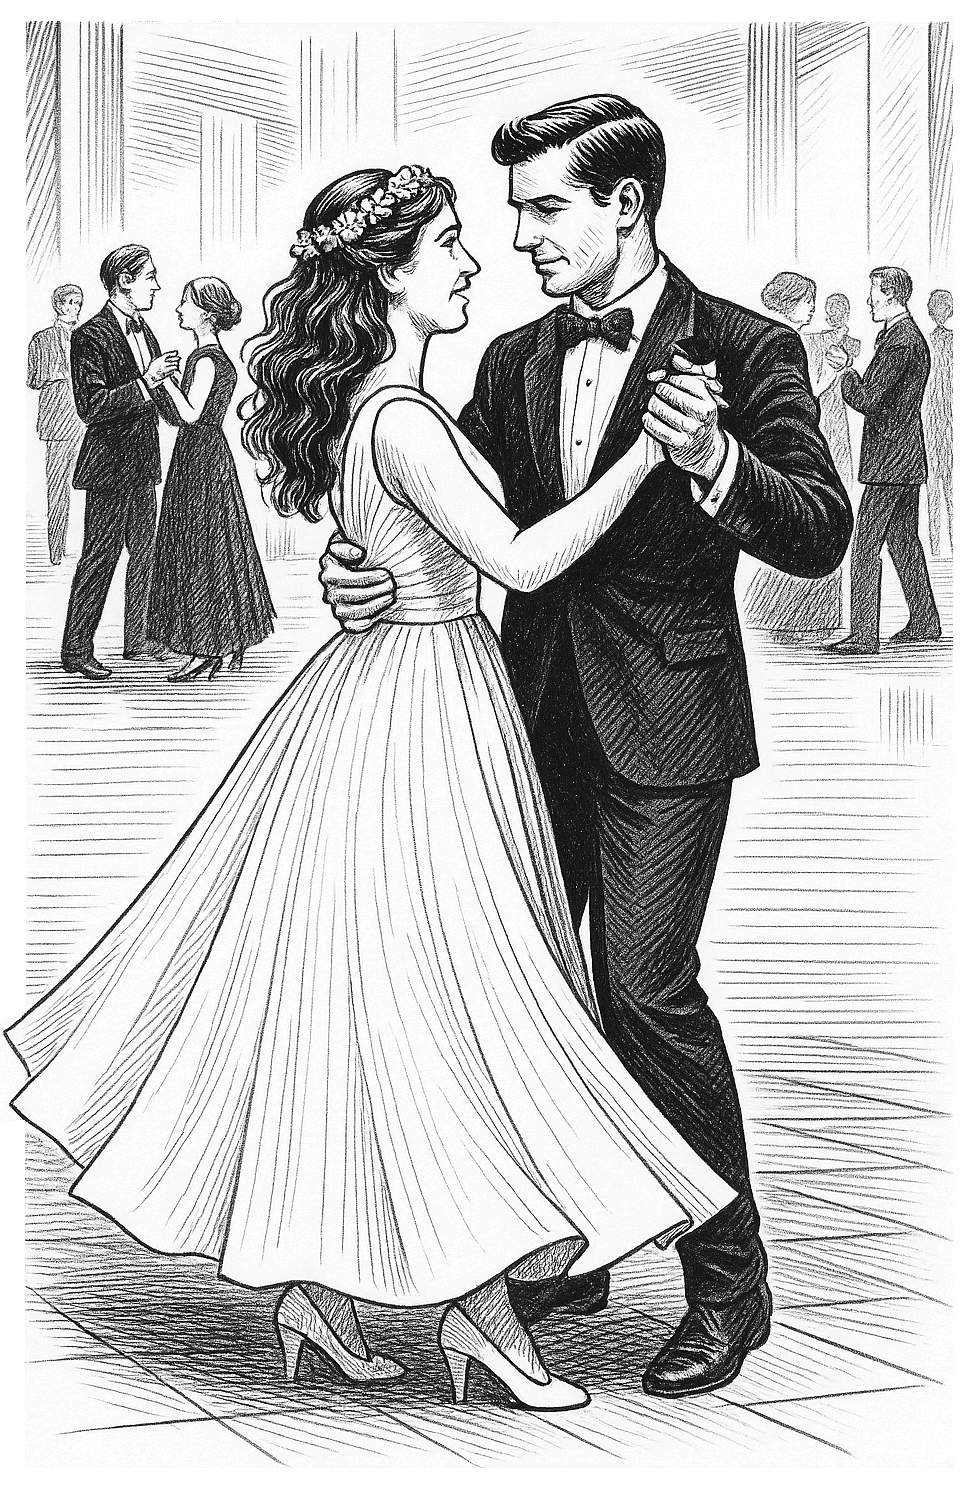
\includegraphics[width=\linewidth]{02_wedding}
	
	{\small\textit{...в платье белом...}}
\end{minipage}

%----------------------------------------------------------------
% 3 ГЛАВА
%----------------------------------------------------------------
\newpage

\begin{figure}[h]
\centering
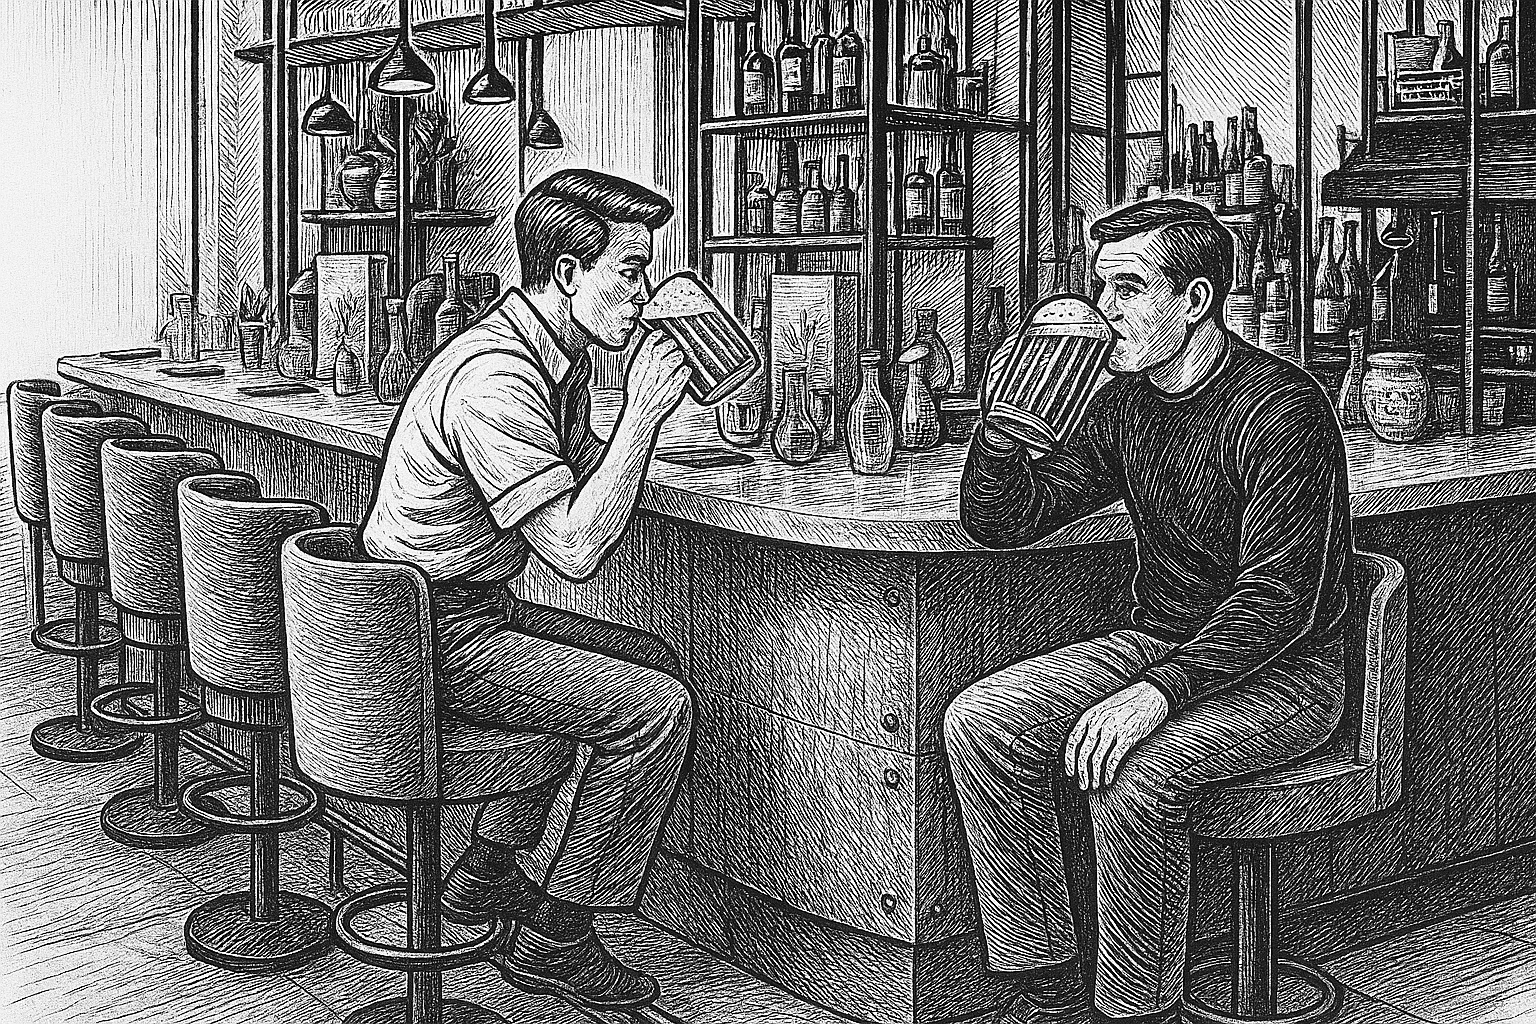
\includegraphics[width=1.0\textwidth]{03_beer}
\caption{\small\textit{...Адмирал с Замполитом сидели в пивнушке...}}
\end{figure}

%----------------------------------------------------------------
\newpage

\noindent
\begin{minipage}{0.55\textwidth}
	\setlength{\parindent}{1.0cm}  % Включаем красную строку
	\setlength{\parskip}{0.25cm}     % Межабзацный отступ, как в основном тексте
	
	\noindent байдарочных фартука, надев их на себя. Узнал издалека, не~ошиблась.
	
	\diagdash Так, вот, держите,\mdash стала передавать, снимая с~себя снарягу, байдарочница, а~Шурик стал навешивать фартуки и~жилеты уже на~себя.
	
	\diagdash А остальное?	
	
	\diagdash А остальное на другом складе, надо пройти минут пять, пошли?\mdash маняще мотнула она головой в~сторону 9\sdash этажек и~поправила волосы$\ldots$
\end{minipage}\hfill
\begin{minipage}{0.40\textwidth}
	\centering
	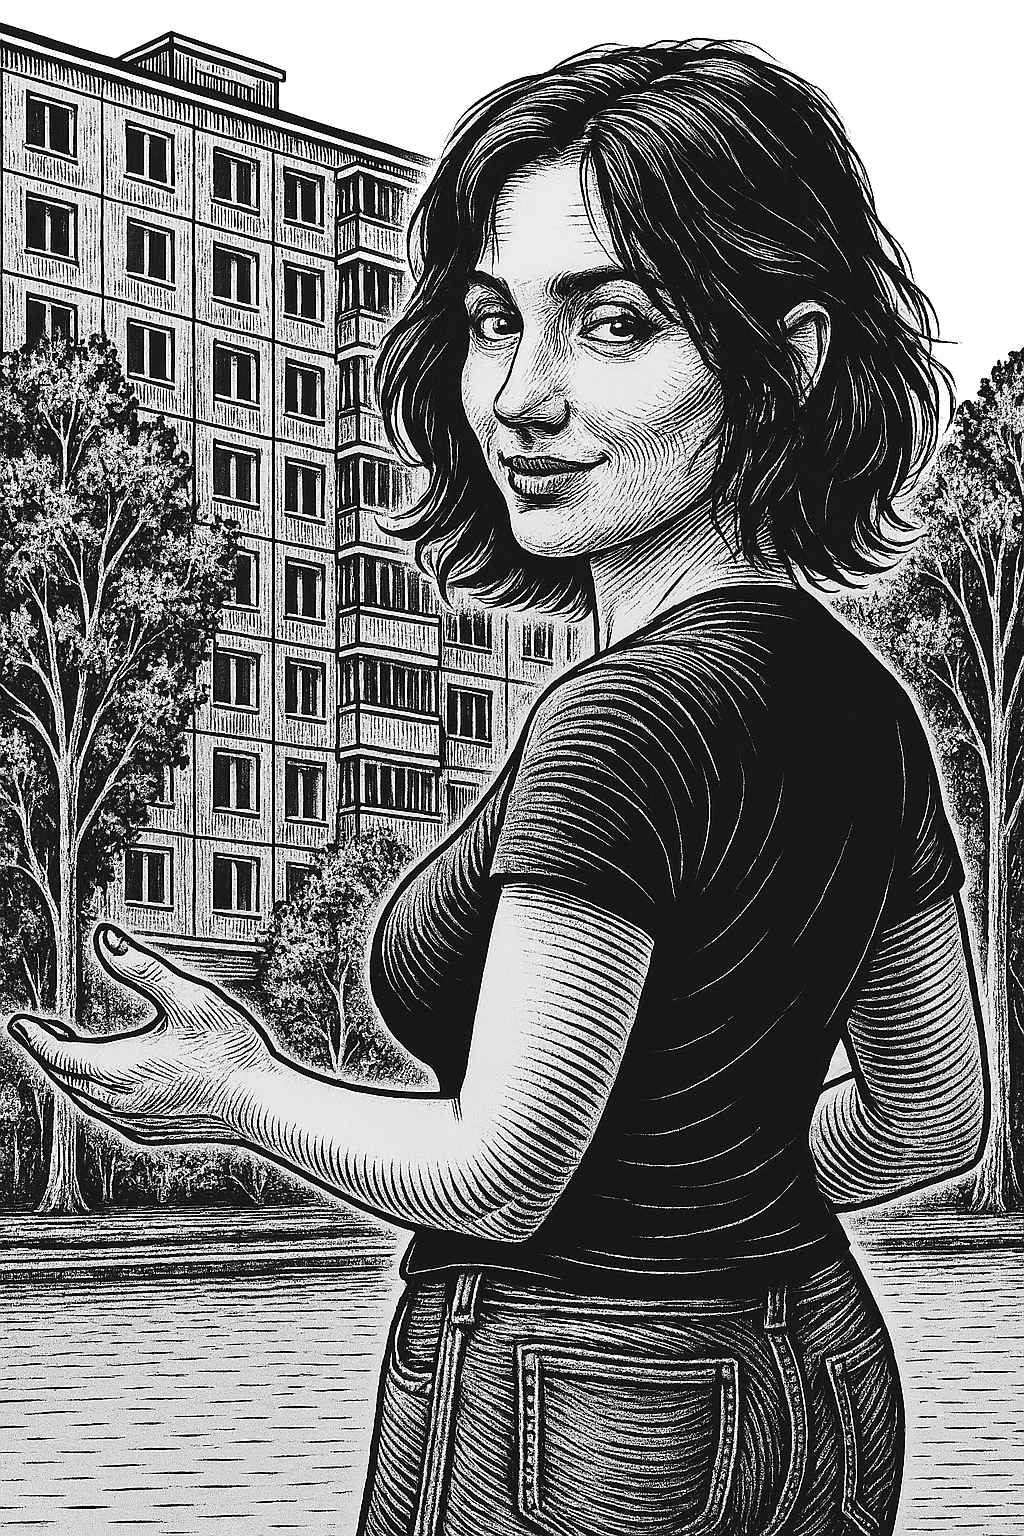
\includegraphics[width=\linewidth]{04_girl}
	
	{\small\textit{...с~хитрым~прищуром...}}
\end{minipage}

%----------------------------------------------------------------
\newpage

\begin{wrapfigure}[11]{l}{0.49\textwidth}
	%\begin{figure}[h]
	\centering
	%	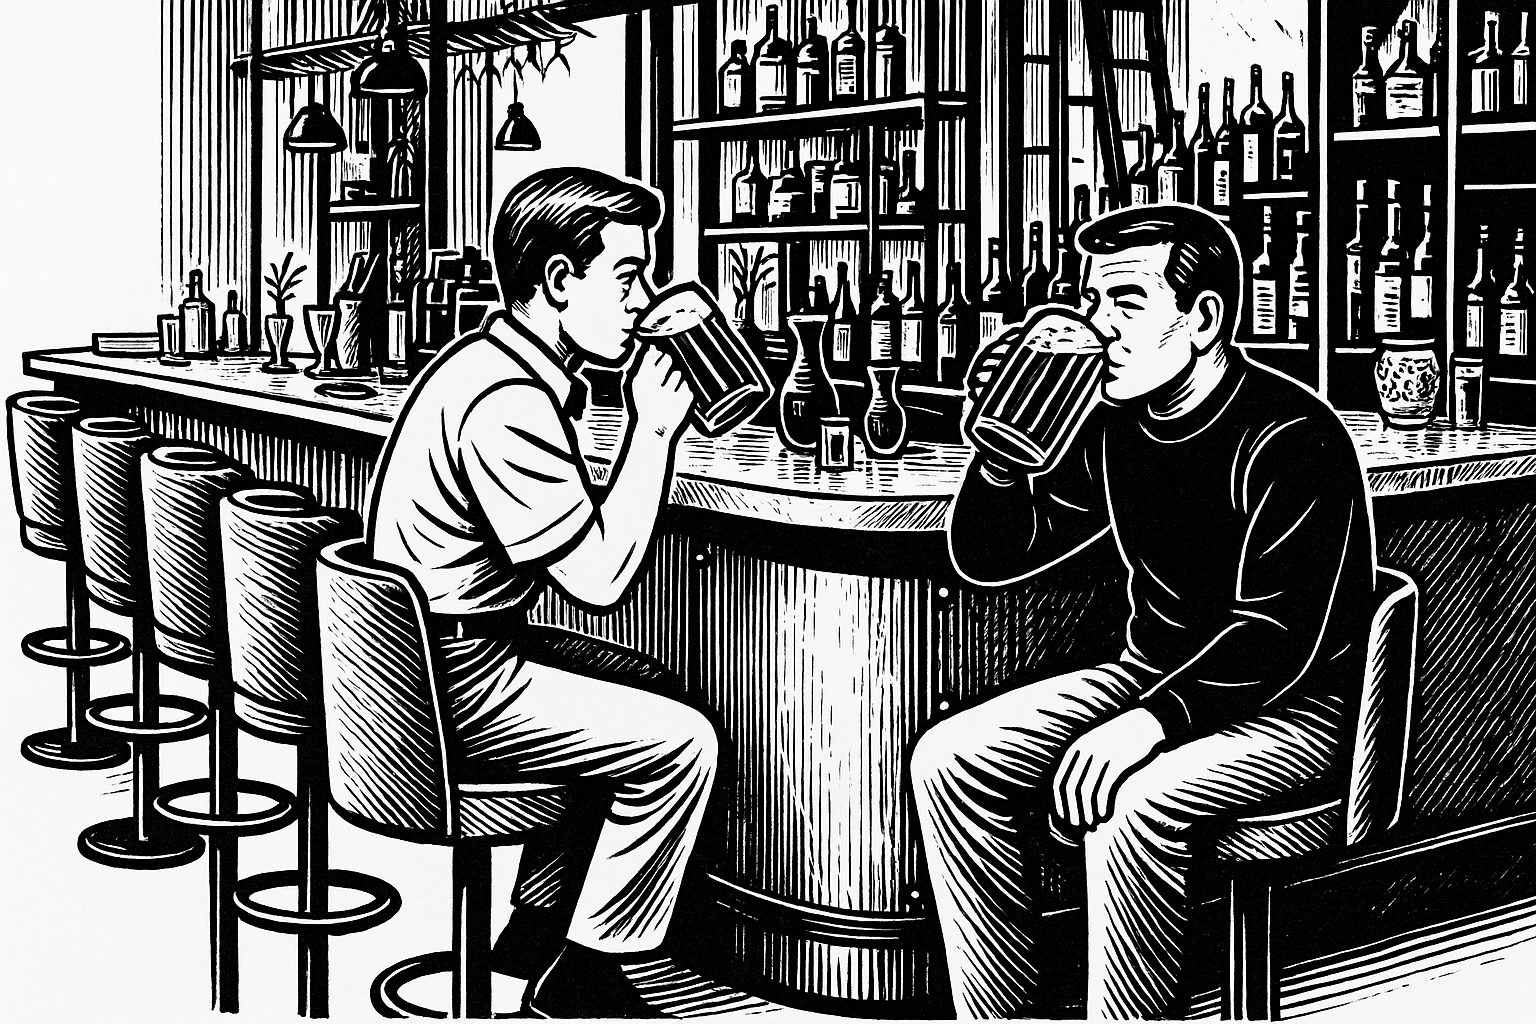
\includegraphics[width=1.0\textwidth]{3_new3}
	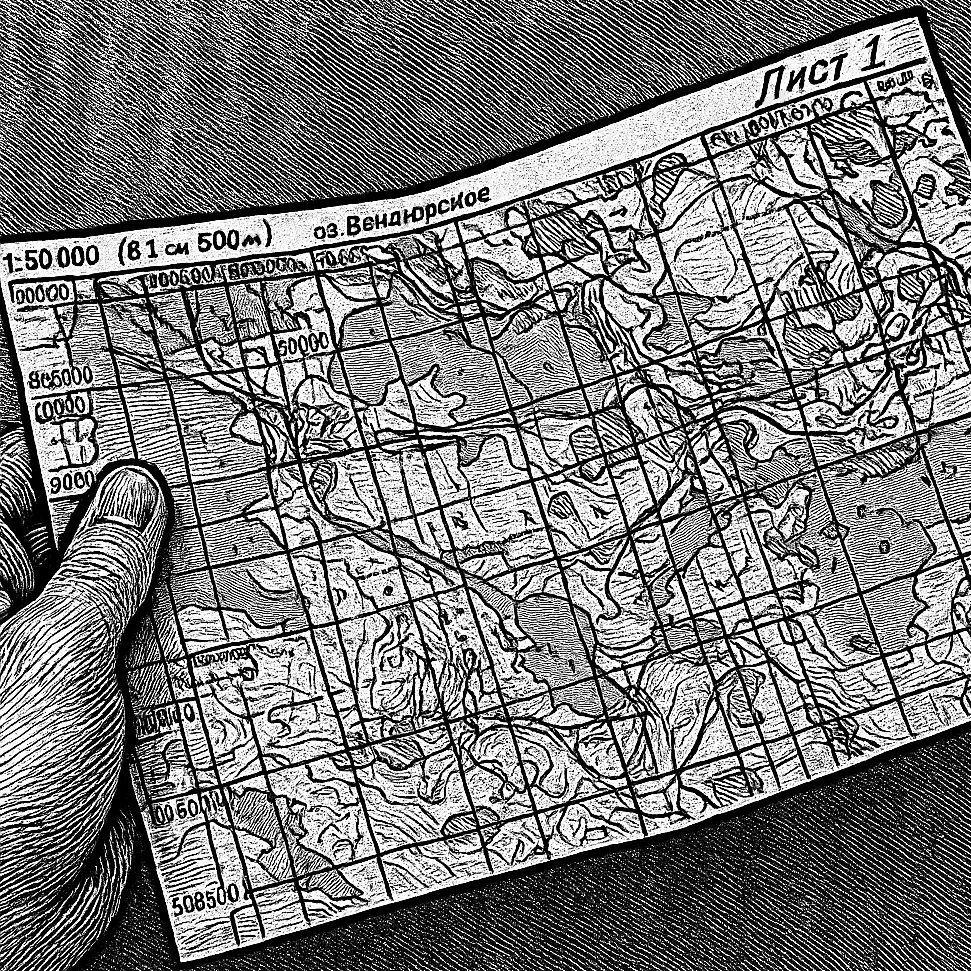
\includegraphics[width=0.47\textwidth]{05_map}
	\caption{\small\textit{...повело плёнку...}}
	%\end{figure}
\end{wrapfigure}

\diagdash А~дубликат~есть?\mdash заволновалась Надя.

\diagdash Нет уж, пойдём по такой карте.\mdash Замполит деланно закатил глаза.\mdash Потеряемся, как пить дать! Ё\sdash моё! Ну всё, Шурик, по~такой карте идти нельзя! 

\diagdash Всё пропало, Кирь!\mdash подыграл тот.


%----------------------------------------------------------------
% 4 ГЛАВА
%----------------------------------------------------------------

%\newpage
\vspace{20mm}

\begin{figure}[h]
	\centering
	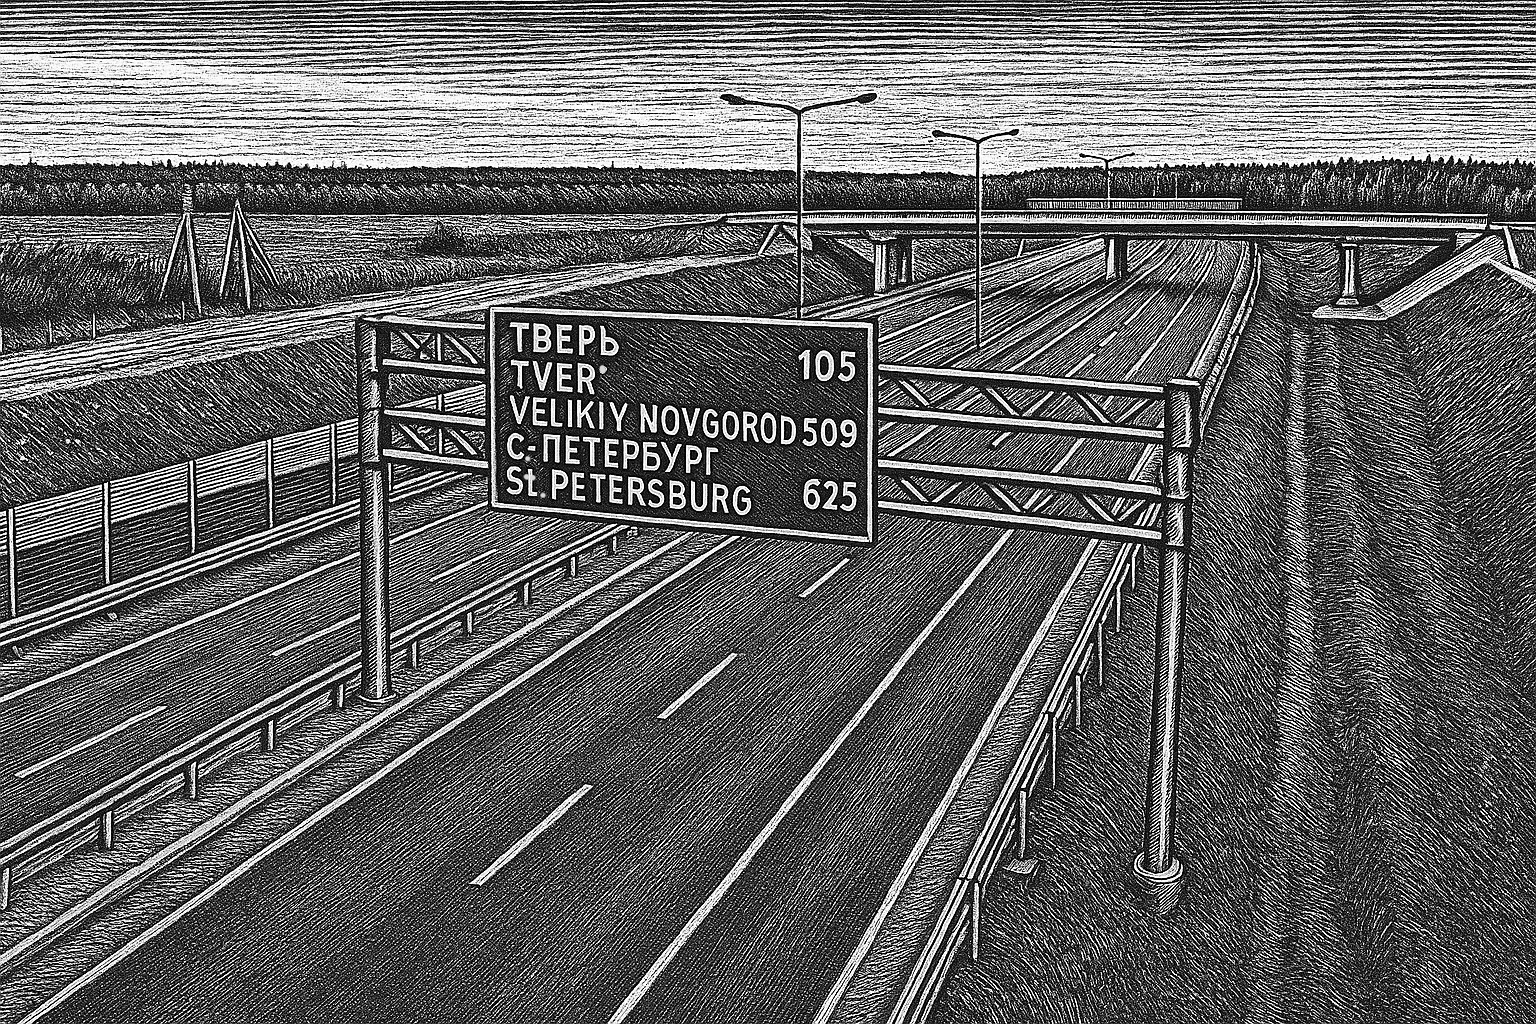
\includegraphics[width=1.0\textwidth]{06_highway}
	\caption{\small\textit{...бодро рванул вперёд по автостраде, утапливая педаль газа...}}
\end{figure}

%----------------------------------------------------------------
% 5 ГЛАВА
%----------------------------------------------------------------
\newpage

\begin{figure}[h]
\centering
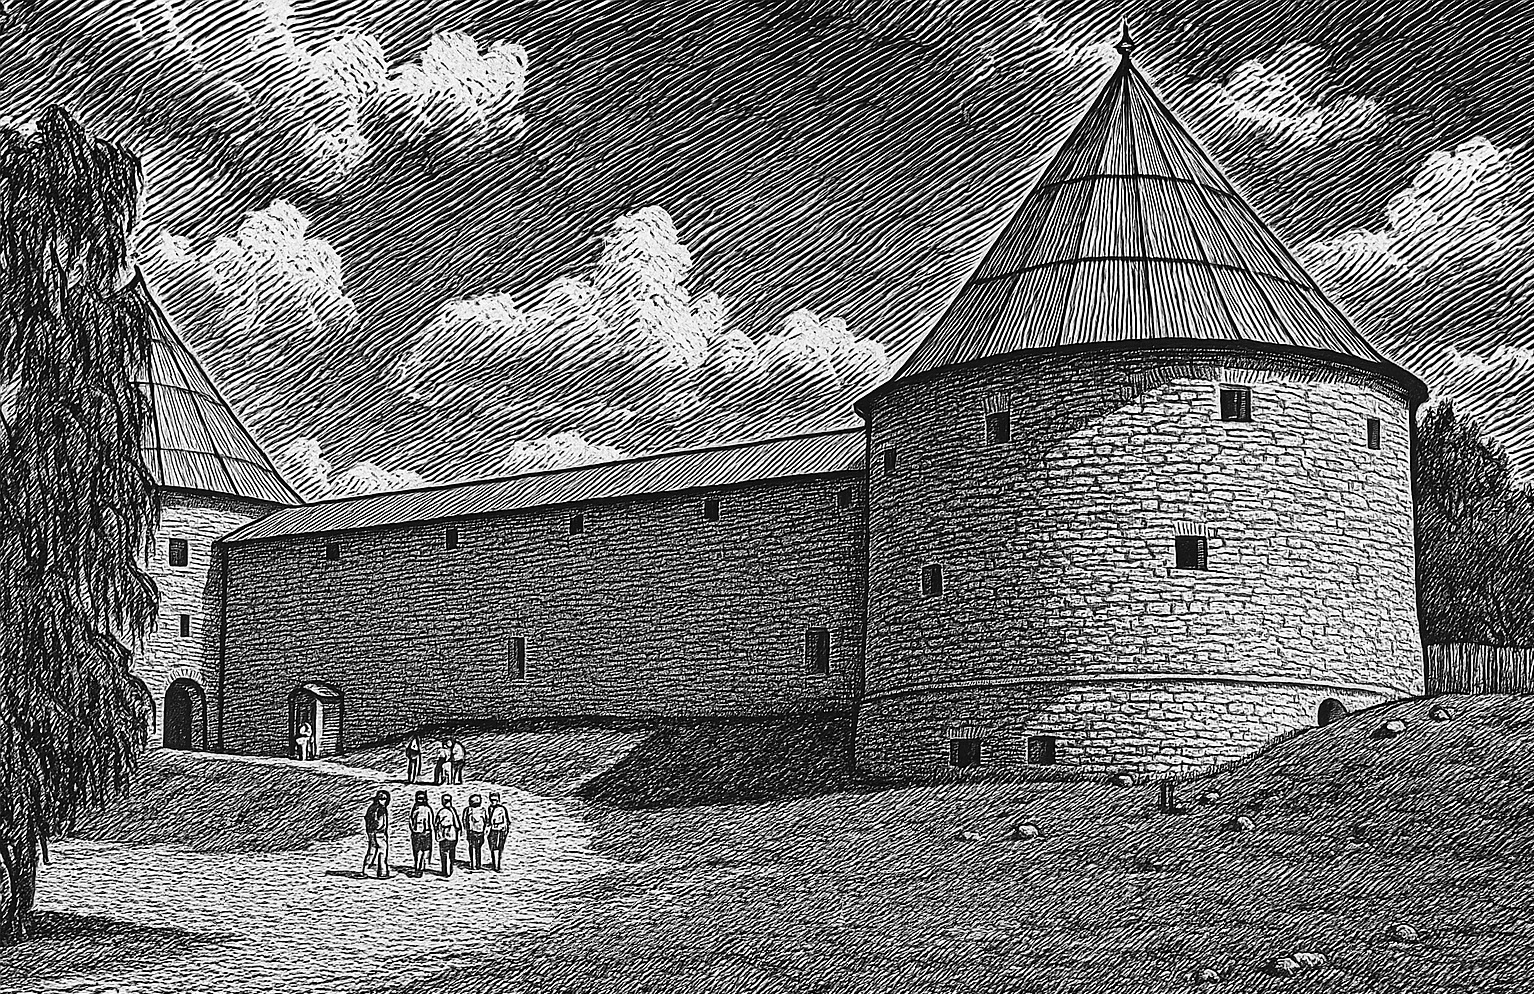
\includegraphics[width=1.0\textwidth]{07_ladoga}
\caption{\small\textit{...нет, не скифы, не азиаты мы...}}
\end{figure}

%----------------------------------------------------------------
\newpage

text text

\noindent
\begin{minipage}{0.45\textwidth}
	\setlength{\parindent}{1.0cm}  % Восстановление отступа абзаца
	
	\indent Смотровая площадка располагалась после 4-й ступени водопада, самой высокой, а~немного выше был виден предыдущий каскад с~двумя чуть меньшими водопадиками. Друзья забрались в~самый дальний край тропинки на~гору, где была установлена лавочка и~открывался чудесный вид вниз на~долину. Присели на лавочку передохнуть и~подождать Серёгу с~Русланом.
	
	\indent Кивач\mdash жемчужина Карелии. Заповедник был \makebox[\linewidth][s]{\noindent создан в~30\sdash ые годы XX\hspace{0.25em}в.}
\end{minipage}\hfill
\begin{minipage}{0.5\textwidth}
	\centering
	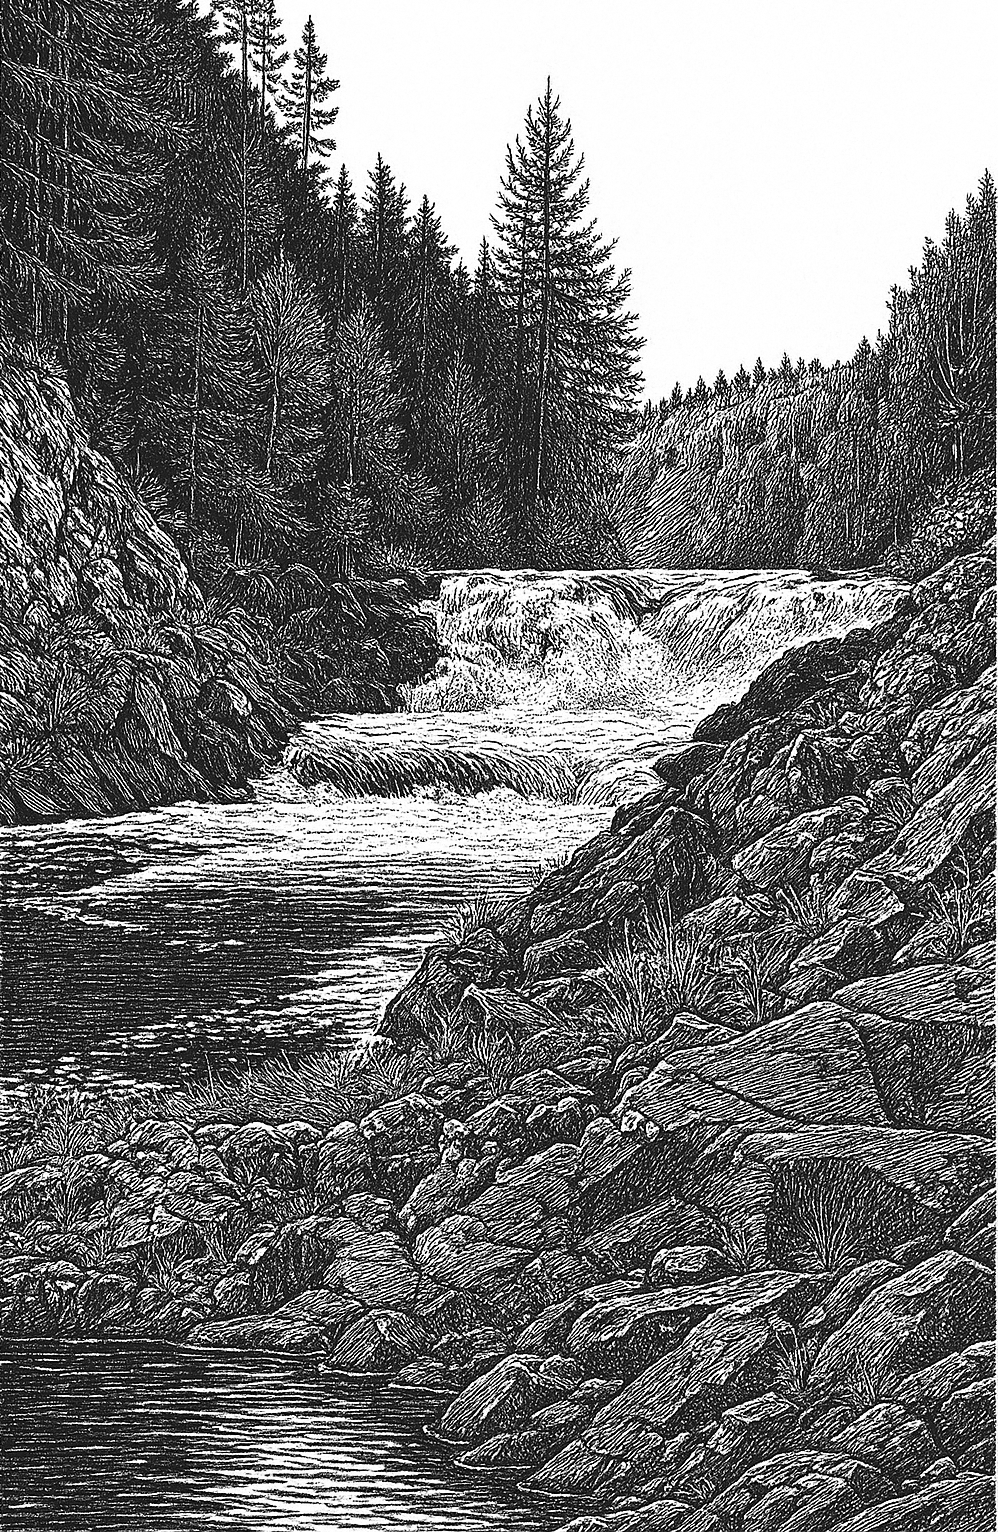
\includegraphics[width=\linewidth]{08_kivach}
	
	{\small\textit{...жемчужина Карелии...}}
\end{minipage}

%----------------------------------------------------------------
\newpage

\begin{figure}[h]
	\centering
	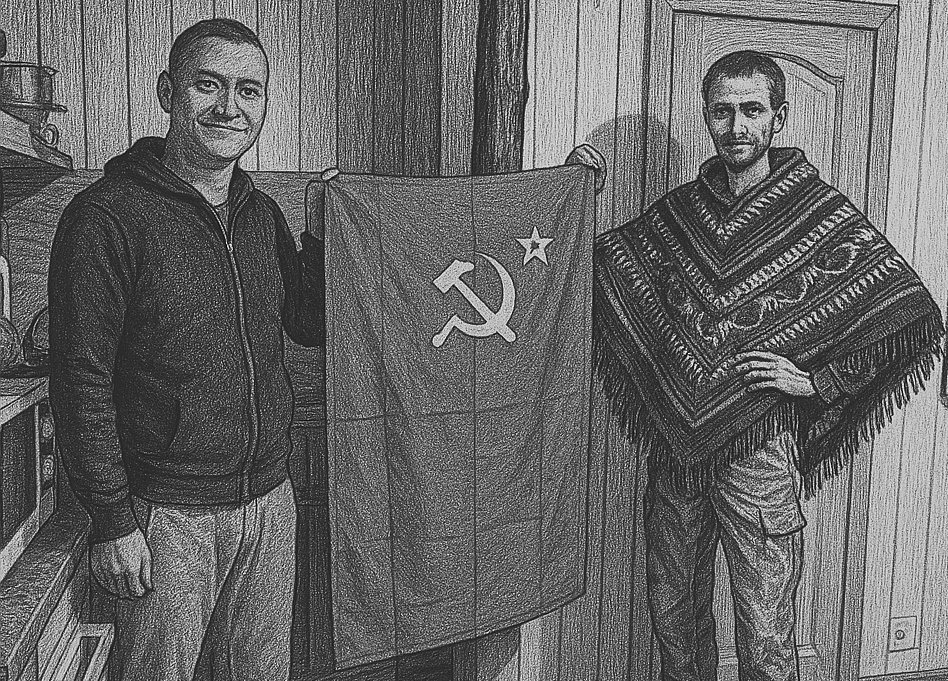
\includegraphics[width=1.0\textwidth]{09_ussr}
	\caption{\small\textit{...молоткасто-серпастое...}}
\end{figure}

%----------------------------------------------------------------
% 6 ГЛАВА
%----------------------------------------------------------------
\newpage

\begin{figure}[h]
	\centering
	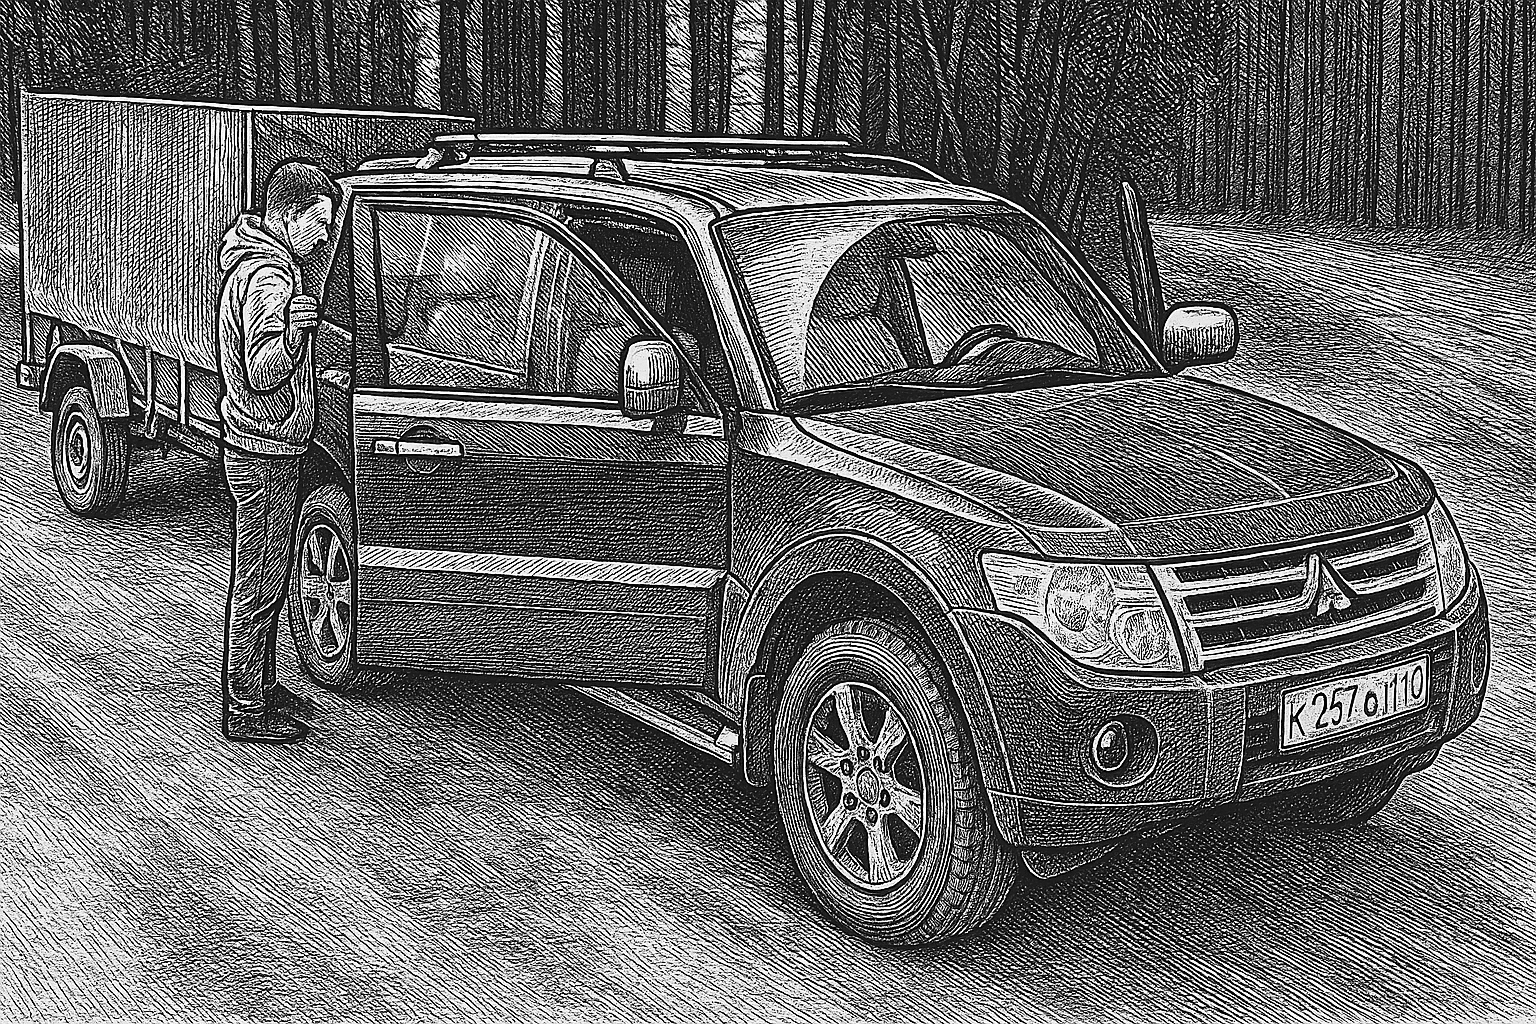
\includegraphics[width=1.0\textwidth]{10_jeep}
	\caption{\small\textit{...свернули направо на Нёлгомозеро...}}
\end{figure}

abcd

\begin{figure}[h]
	\centering
	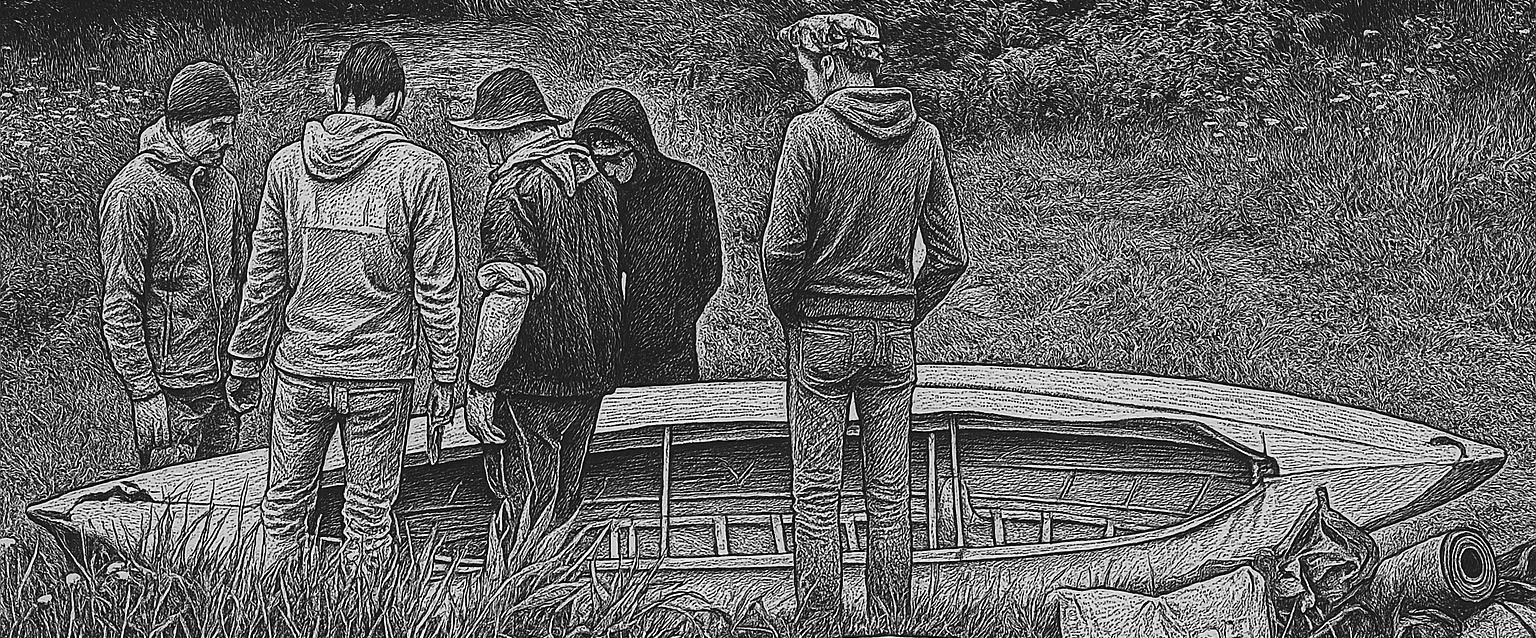
\includegraphics[width=1.0\textwidth]{11_keelson}
	\caption{\small\textit{...фальшборт не лезет...}}
\end{figure}

%----------------------------------------------------------------
\newpage

\begin{figure}[h]
	\centering
	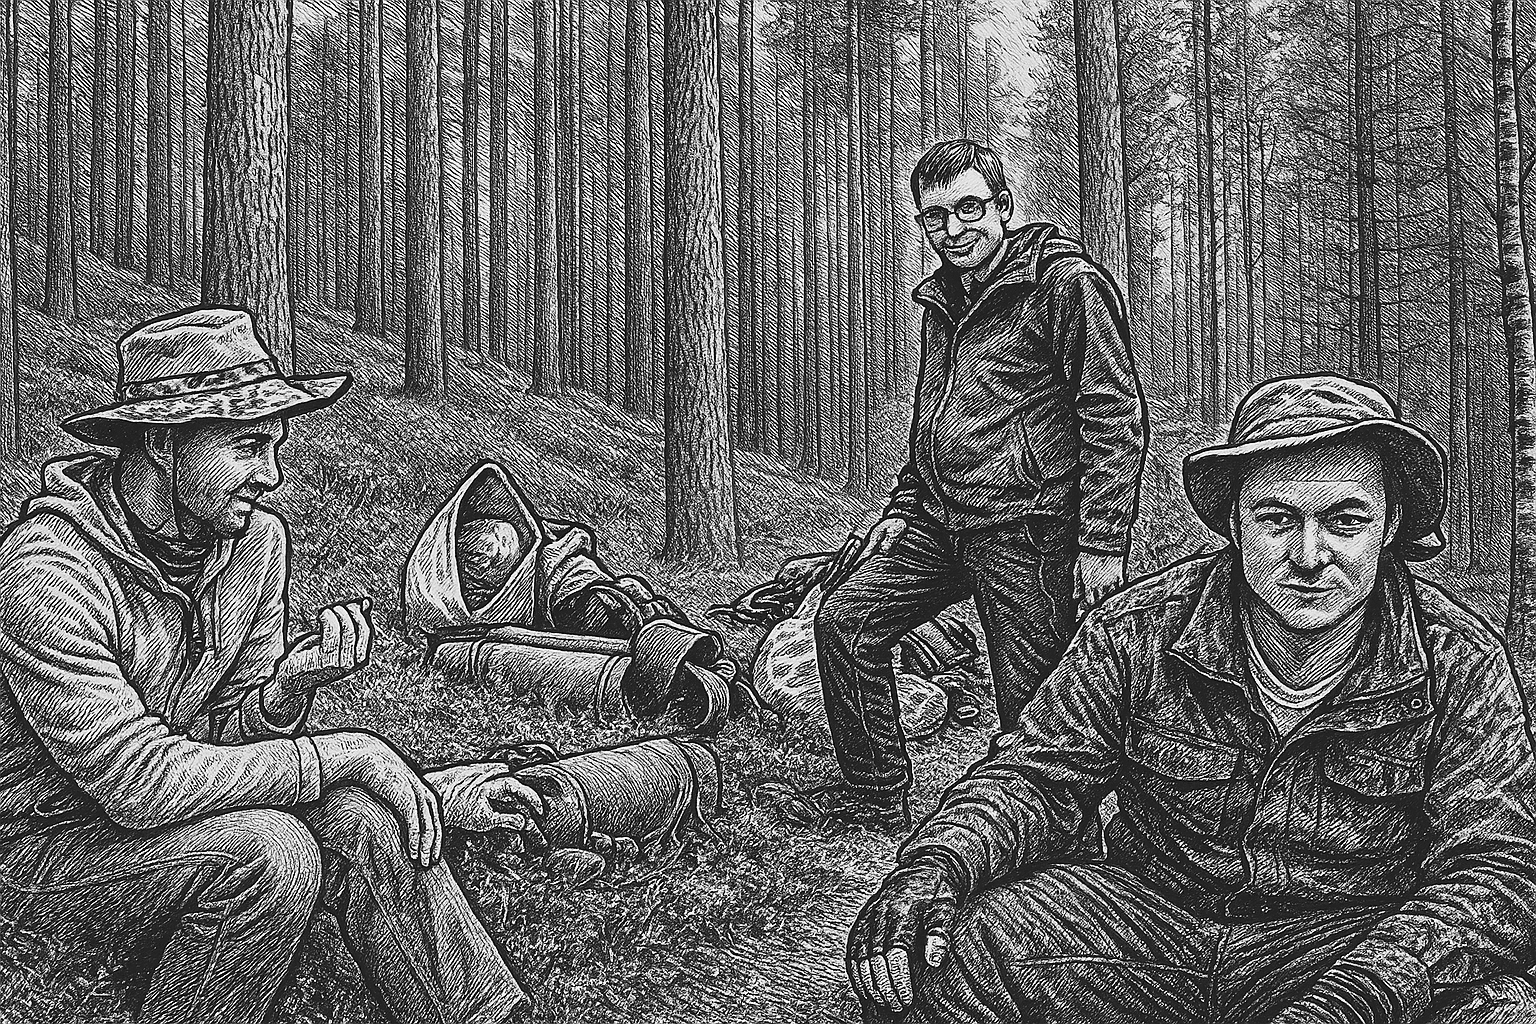
\includegraphics[width=1.0\textwidth]{12_maybe}
	\caption{\small\textit{...А чё, давайте может?...}}
\end{figure}

abcd

\newpage

\begin{wrapfigure}[10]{l}{0.52\textwidth}
	\setlength{\belowcaptionskip}{-10pt}
	%	\begin{figure}[h]
		\centering
		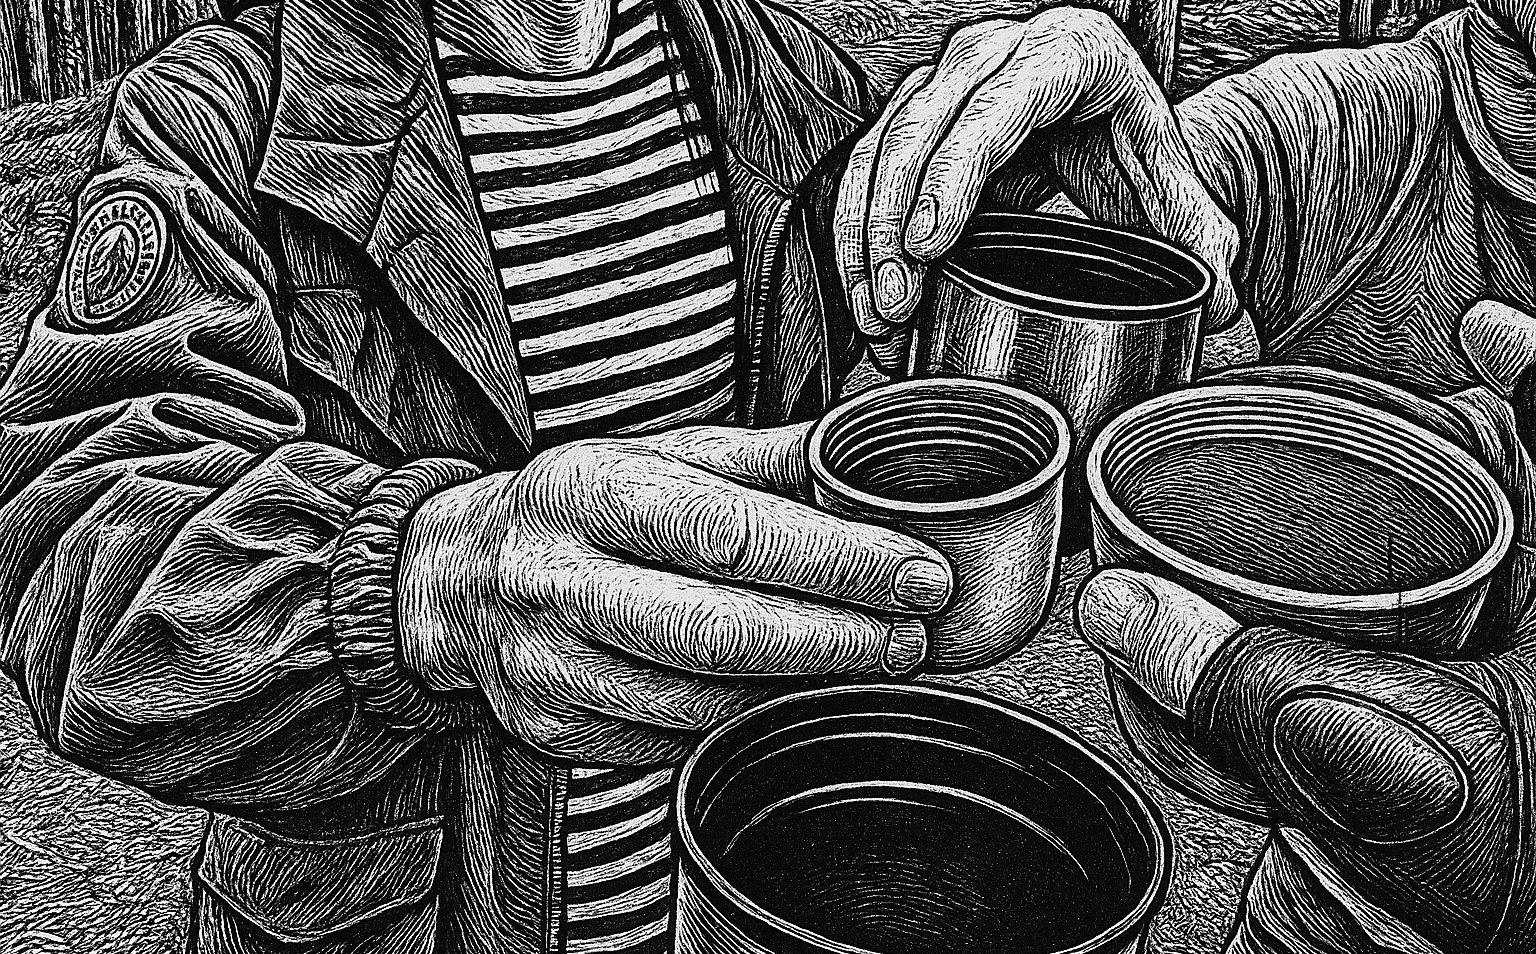
\includegraphics[width=0.52\textwidth]{13_skol}
		\caption{\small\textit{...два отрывистых...}}
		%	\end{figure}
\end{wrapfigure}

\noindent И сегодня нас ждут каналы между озёрами ещё, кстати. Итак, то, к~чему мы стремились\mdash свершается! Мы выбрались в наш первый совместный сплав по Карелии и, надеюсь, это приключение запомнится нам надолго! Ну,~мужики, будем!\mdash лес рук с кружками поднялся и замер, ожидая команды.\mdash Тащ~Замполит, два отрывистых и одно раскатистое!!!

%----------------------------------------------------------------
% 7 ГЛАВА
%----------------------------------------------------------------
\newpage

\begin{figure}[h]
	\centering
	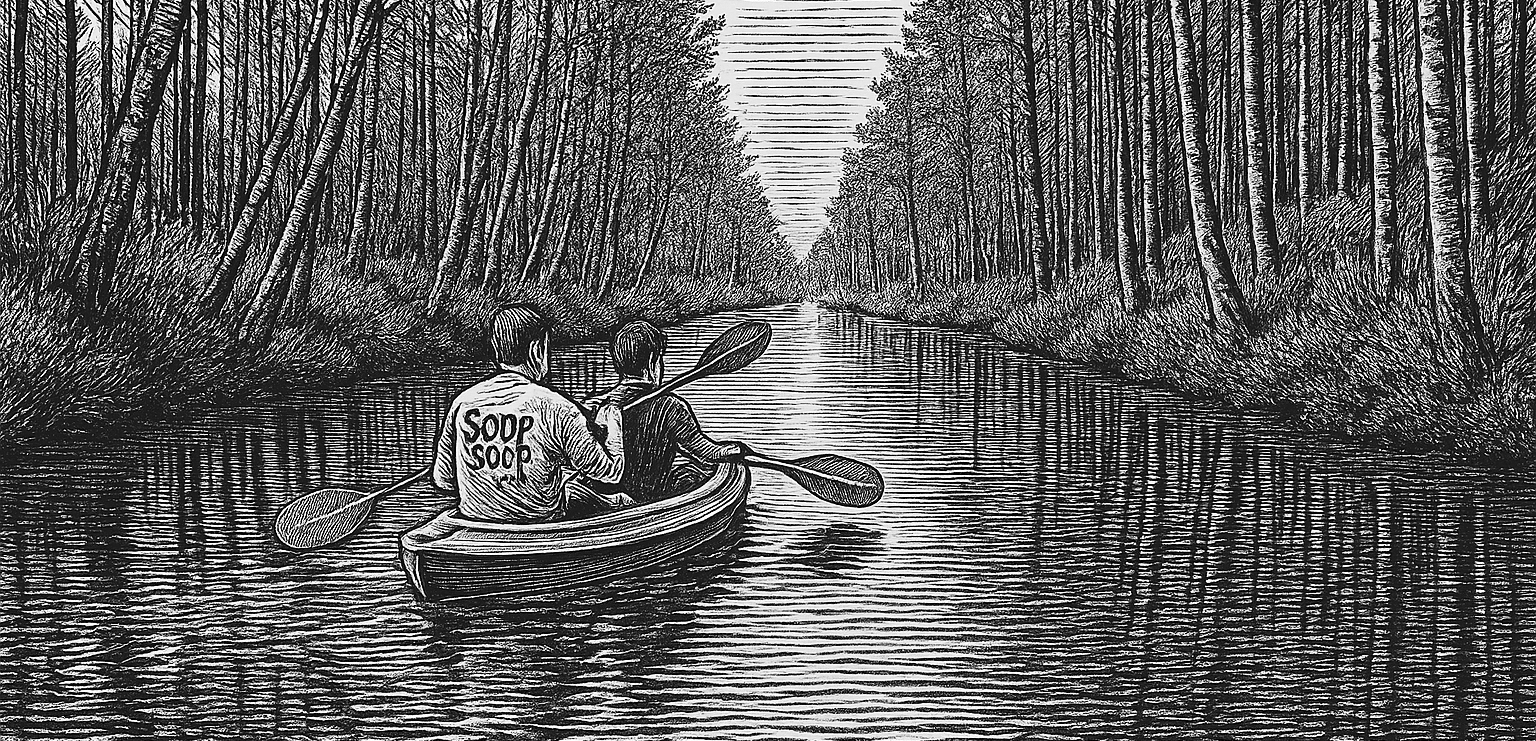
\includegraphics[width=1.0\textwidth]{14_channel}
	\caption{\small\textit{...Канал был шириной примерно метров 8...}}
\end{figure}

%----------------------------------------------------------------
\newpage

\begin{figure}[h]
	\centering
	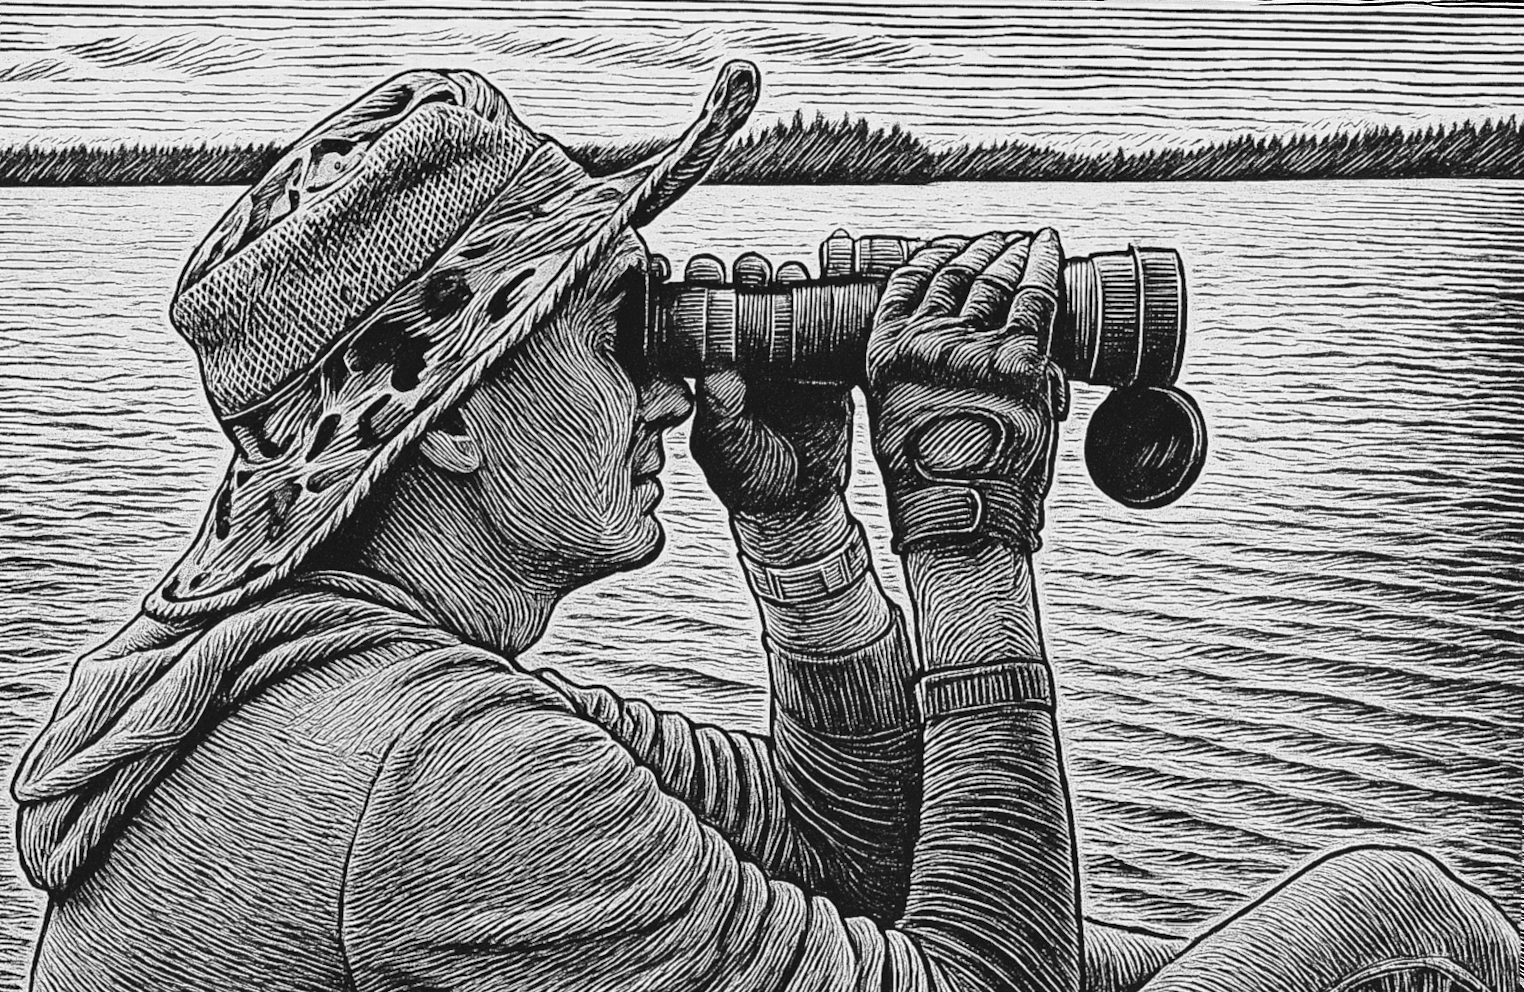
\includegraphics[width=1.0\textwidth]{15_okular}
	\caption{\small\textit{...ты говорил, что у тебя подзорная труба есть?...}}
\end{figure}

%----------------------------------------------------------------
% 8 ГЛАВА
%----------------------------------------------------------------
\newpage

\noindent
\begin{minipage}{0.38\textwidth}
	\setlength{\parindent}{1.0cm}  % Включаем красную строку
	\setlength{\parskip}{0.25cm}     % Межабзацный отступ, как в основном тексте
	
	\vspace{-0.4cm}
	\diagdash И\sdash и\sdash иха! 
	
	\diagdash ПОТАЩИЛО!!! --- Адмирал в полном восторге перестал грести веслом по\sdash байдарочному и~взял его под мышку на манер руля.\mdash Погнали!!!
	
	Ветер дул, конечно, не~особо сильный, но этого было вполне достаточно, чтобы дать им ход в~парочку км/ч. Второй экипаж, тем временем, наконец\sdash то отчалил и~догнал их:
\end{minipage}\hfill
\begin{minipage}{0.57\textwidth}
	\centering
	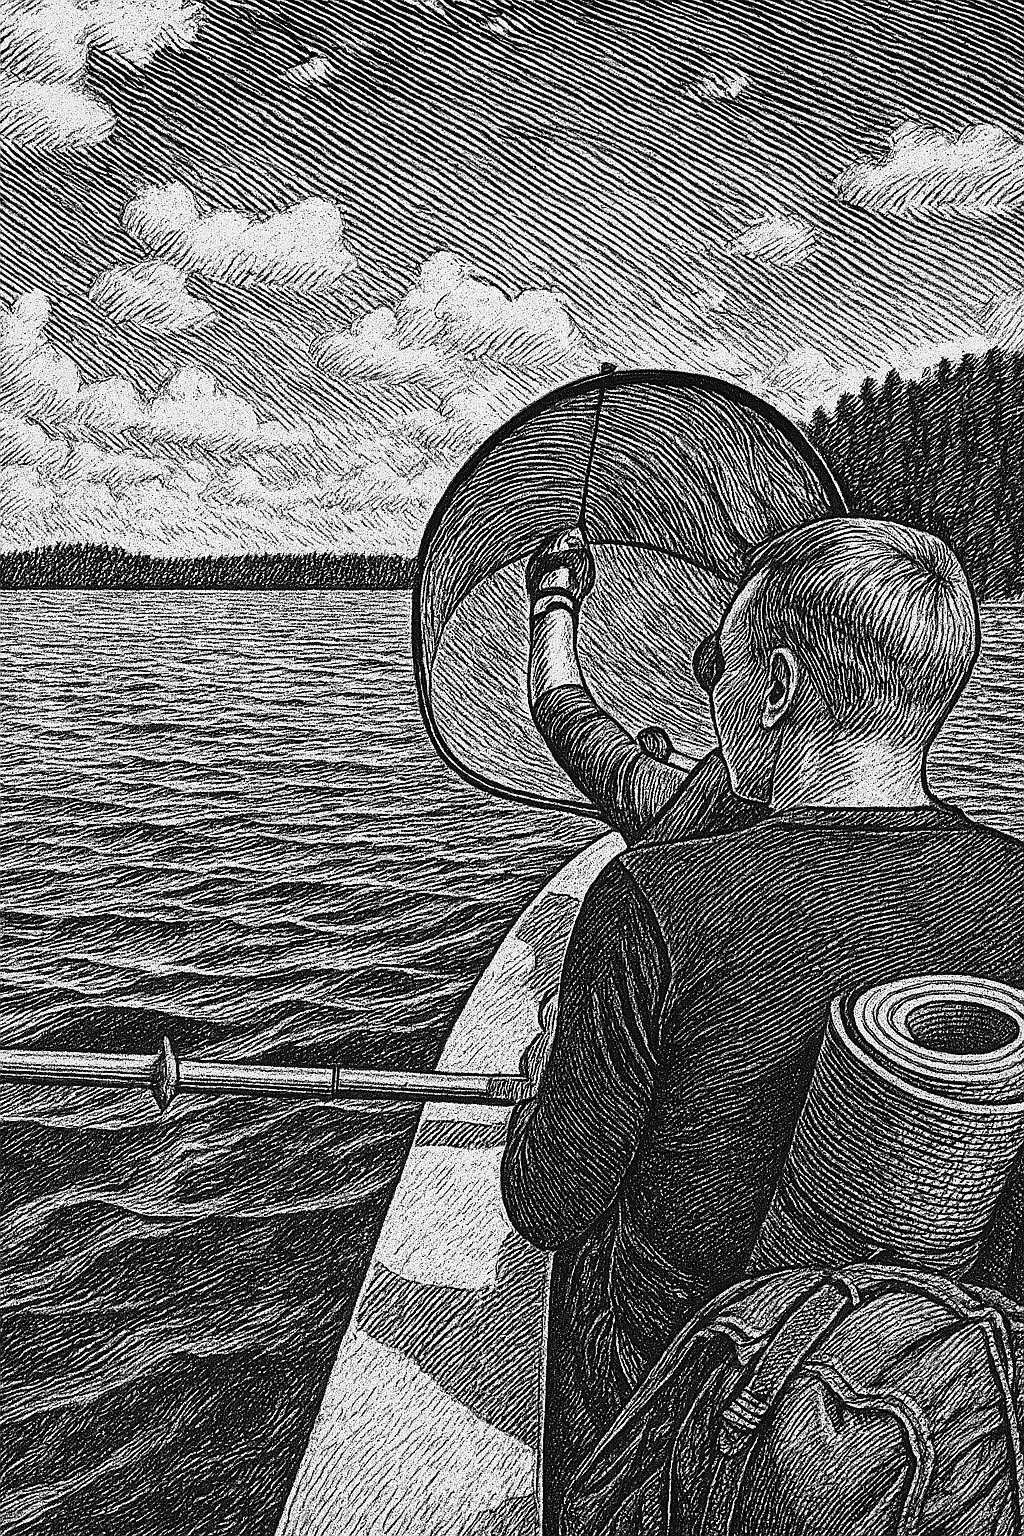
\includegraphics[width=0.95\linewidth]{16_parus}
	
	{\small\textit{...ветер стал усиливаться...}}
\end{minipage}

%----------------------------------------------------------------
\newpage

\begin{wrapfigure}[20]{r}{0.55\textwidth}
	%\begin{figure}[h]
	\centering
	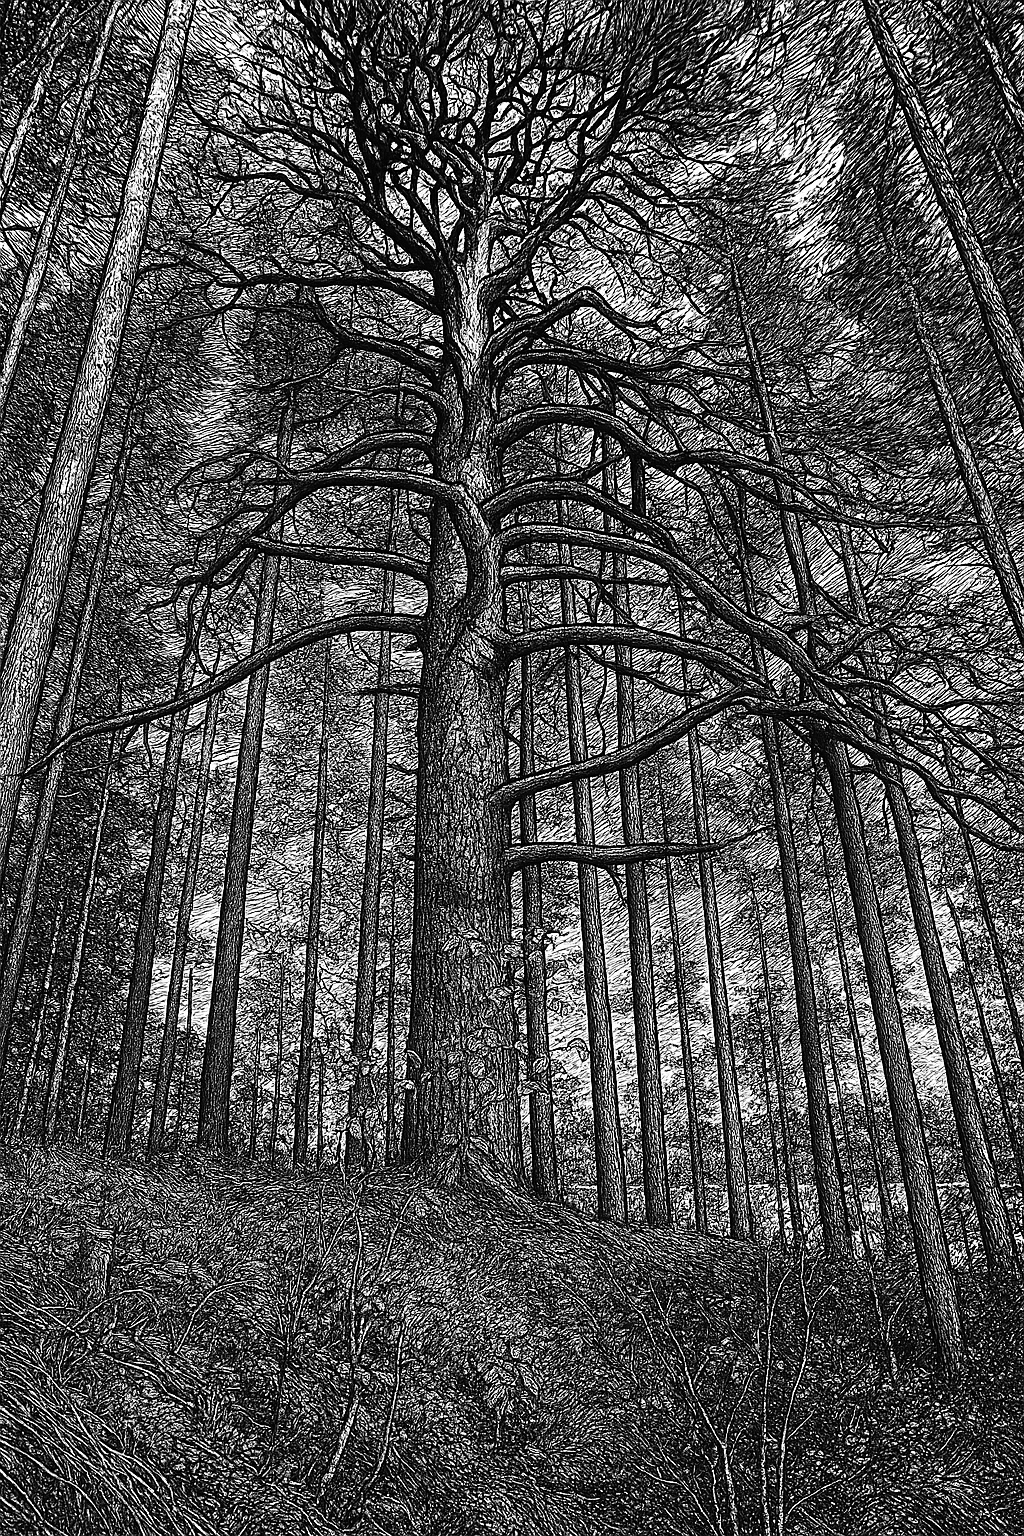
\includegraphics[width=0.55\textwidth]{17_tree}
	\caption{\small\textit{...Мы нашли Иггдрасиль!...}}
	%\end{figure}
\end{wrapfigure}
\diagdash Ваще похоже$\ldots$

\diagdash Шурик, там это, ясень был, у~скандинавов.\mdash сказал подошедший Киря.

\diagdash А у нас сосна будет! Она роднее как\sdash то. Мне всегда нравилась такая мифология\mdash древнегреческая и~древнеримская, потом древнескандинавская$\ldots$ Красиво они всё расписывали, черти!

\diagdash Да ты язычник?

\diagdash Это церковники христианские очернить чтобы придумали\mdash язычники, язычники, тьфу! У меня настольная книга была в школе\mdash <<Легенды и мифы Древней Греции и~Древнего Рима>>\cite{Кун}. Потом на~Скандинавию переключился$\ldots$ Красиво же!

%----------------------------------------------------------------
\newpage

\begin{figure}[h]
	\centering
	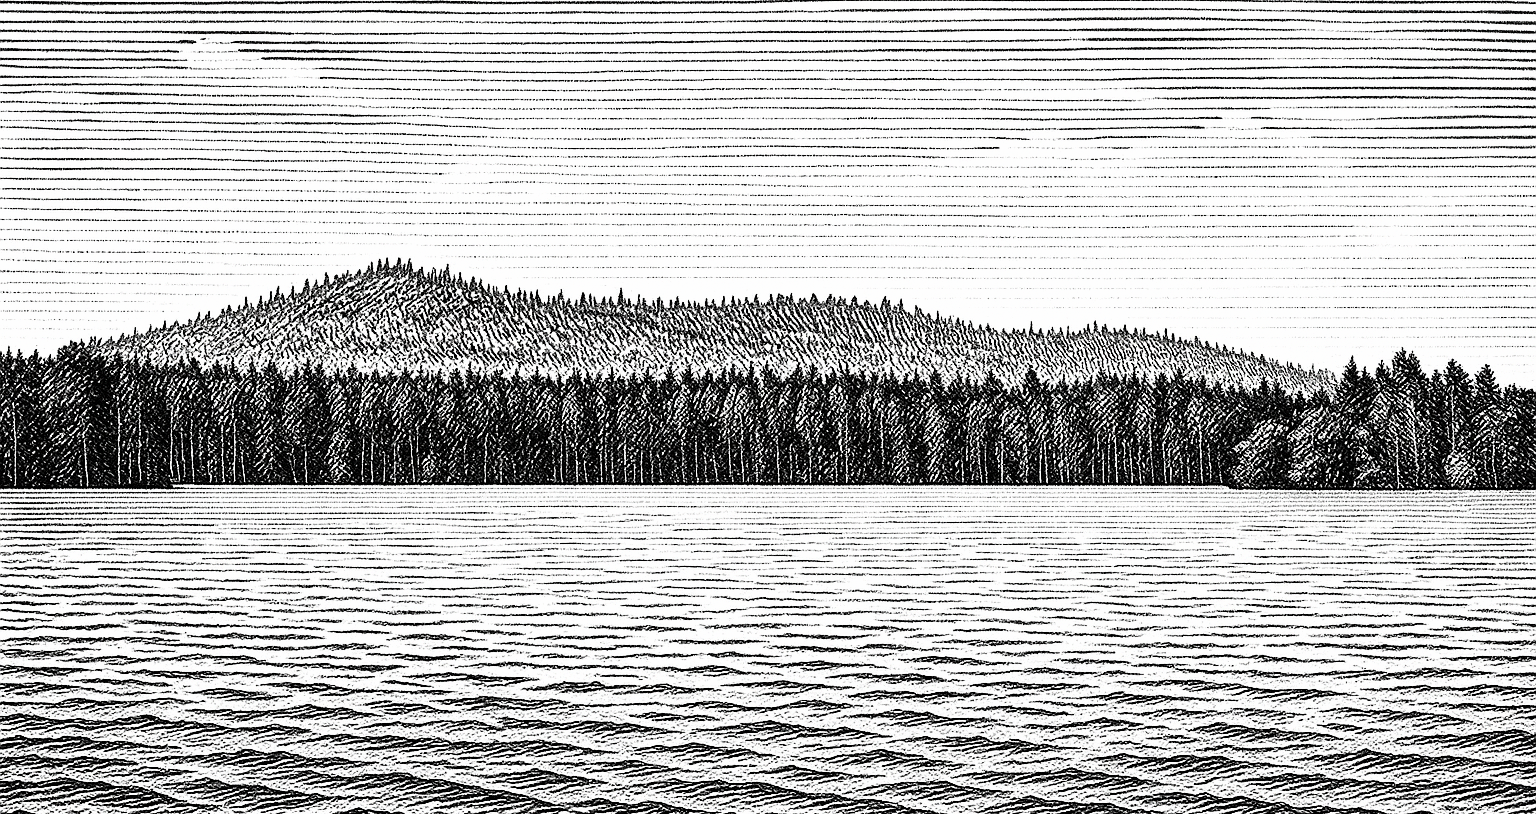
\includegraphics[width=1.0\textwidth]{18_mountain}
	\caption{\small\textit{...На~горизонте виднелась гора Ундойвара...}}
\end{figure}

\begin{wrapfigure}[11]{r}{0.45\textwidth}
	%\begin{figure}[h]
	\centering
	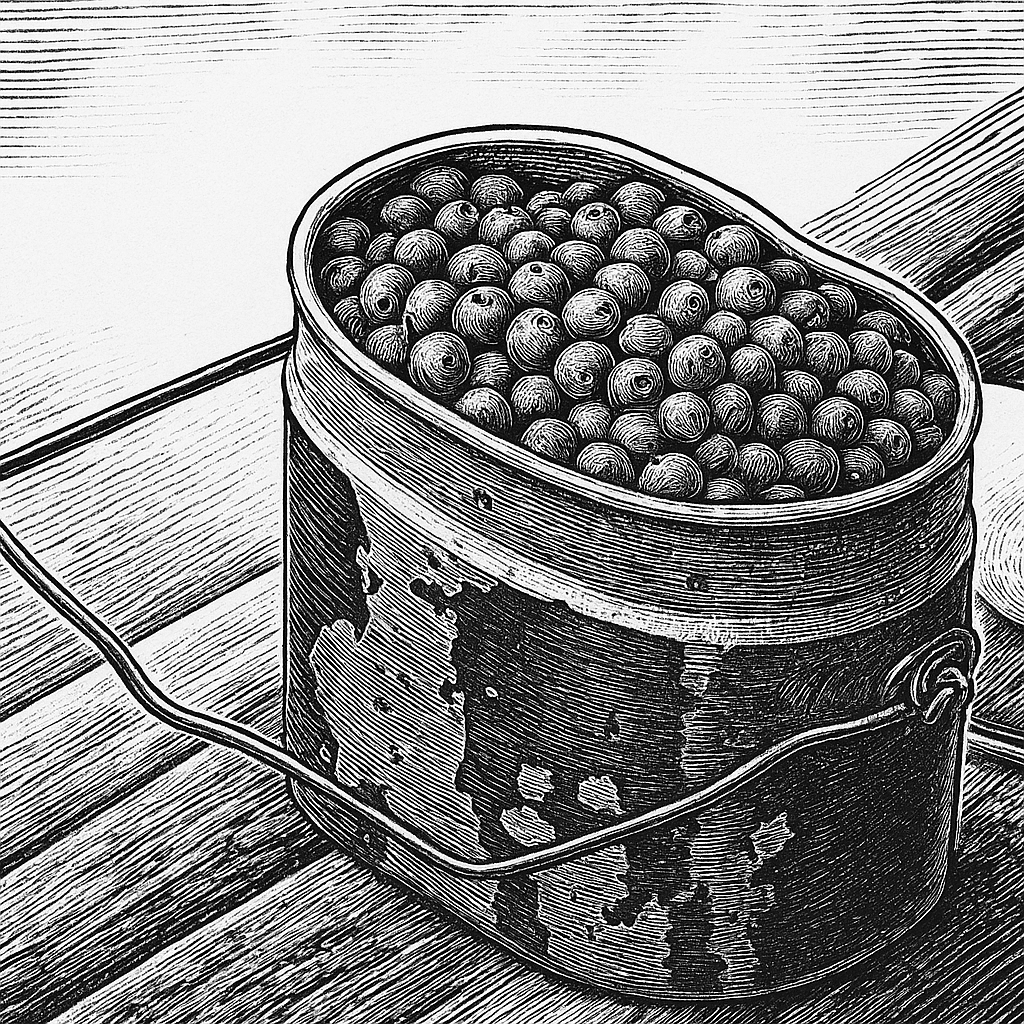
\includegraphics[width=0.45\textwidth]{19_blueberry}
	\caption{\small\textit{...Полный котелок черники...}}
	%\end{figure}
\end{wrapfigure}

%----------------------------------------------------------------
\newpage

\diagdash Не, парни, только троекратное <<УРА>> или <<SKÅL>>!\mdash Адмирал взял дольку апельсинчика.

%\diagdash Не, парни, только расово\sdash чистое троекратное <<УРА>> или <<SKÅL>>!\mdash Адмирал взял апельсинчик.

\diagdash Пофиг, будем!\mdash лес железных кубков поднялся.

\diagdash Кампай!

\diagdash SKÅL! Ну тебя с этим <<кампаем>>! Давай компотик варить!\mdash Адмирал попробовал спелую чернику.

%----------------------------------------------------------------
\newpage

\begin{figure}[h]
	\centering
	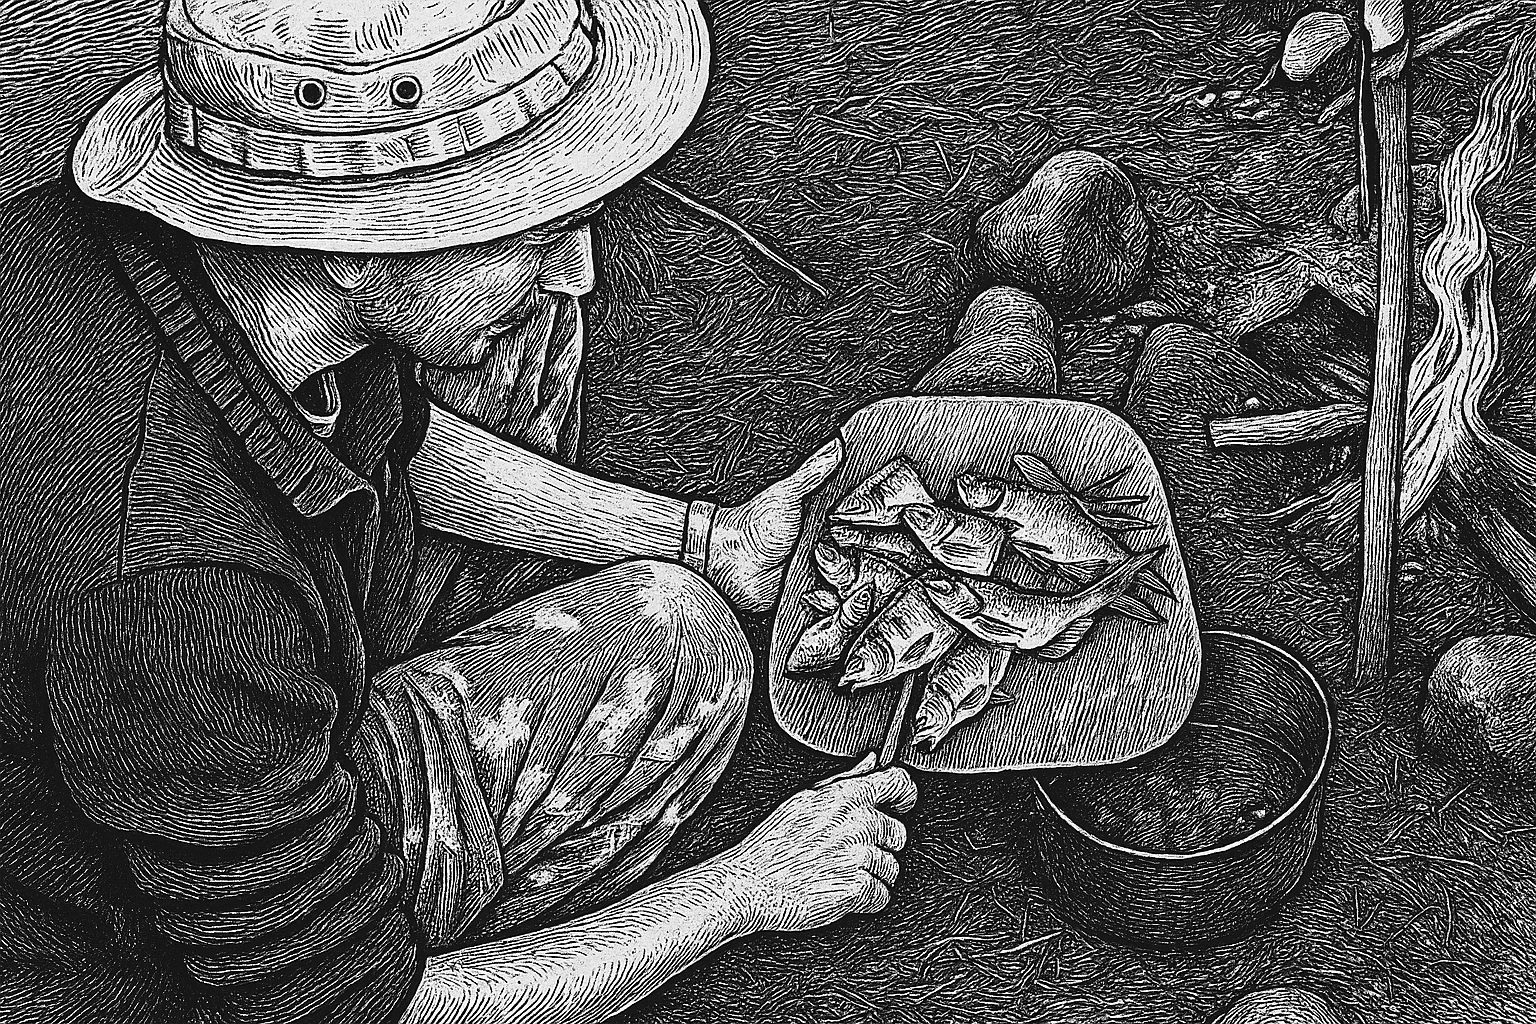
\includegraphics[width=1.0\textwidth]{20_fish}
	\caption{\small\textit{...А что там с супом?...}}
\end{figure}

%----------------------------------------------------------------
\newpage

\begin{figure}[h]
	\centering
	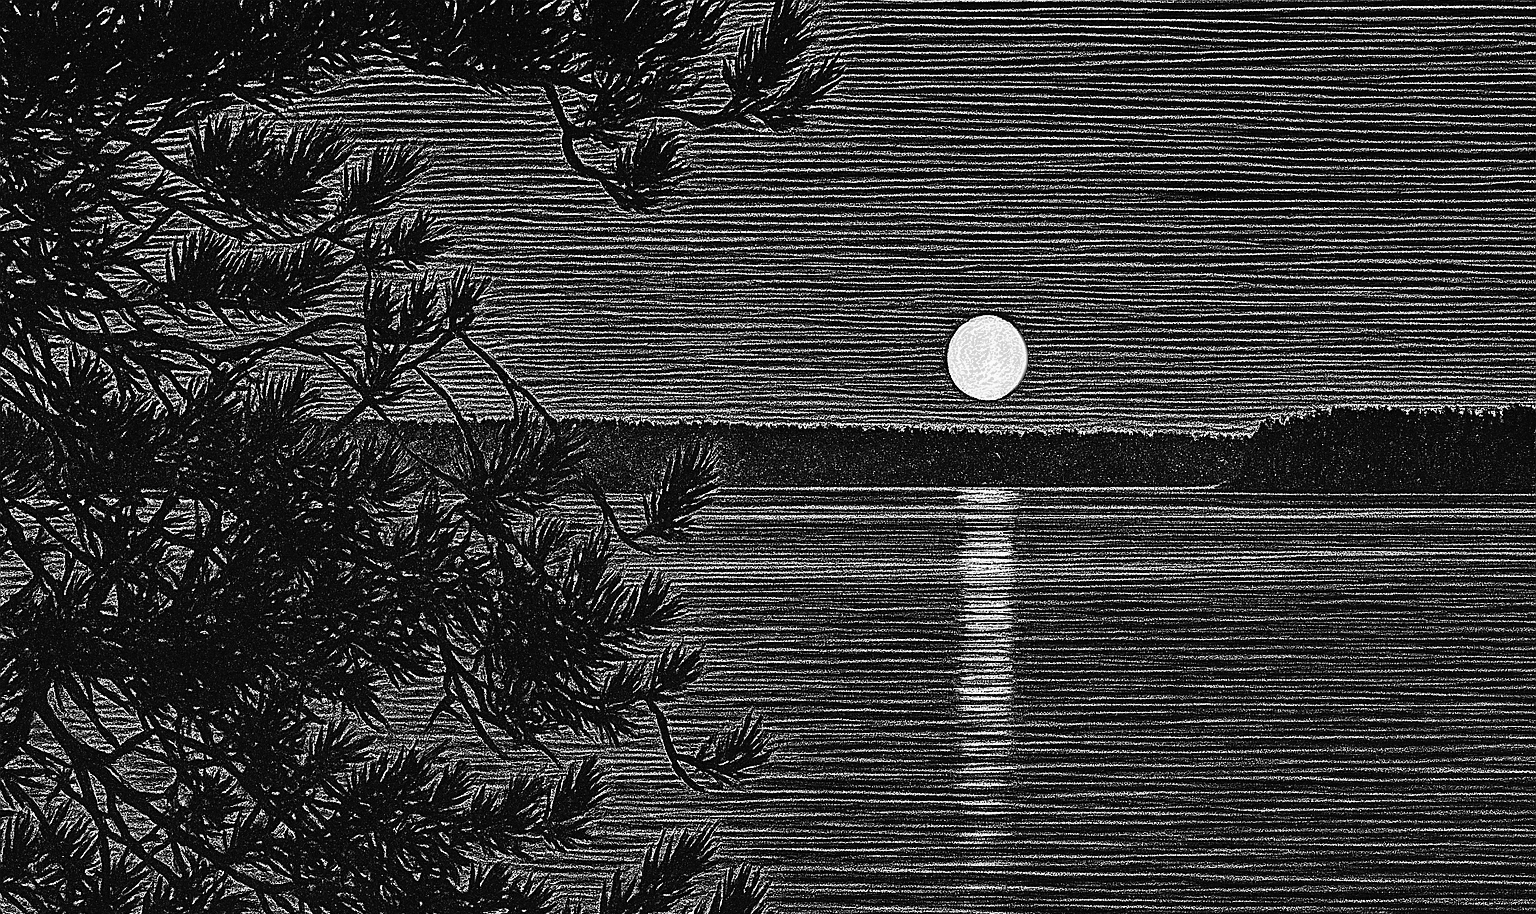
\includegraphics[width=1.0\textwidth]{21_moon.png}
	\caption{\small\textit{...Луна, взошедшая над лесом, отражалась в Мярандуксе...}}
\end{figure}

%----------------------------------------------------------------
% 9 ГЛАВА
%----------------------------------------------------------------
\newpage

\begin{figure}[h]
	\centering
	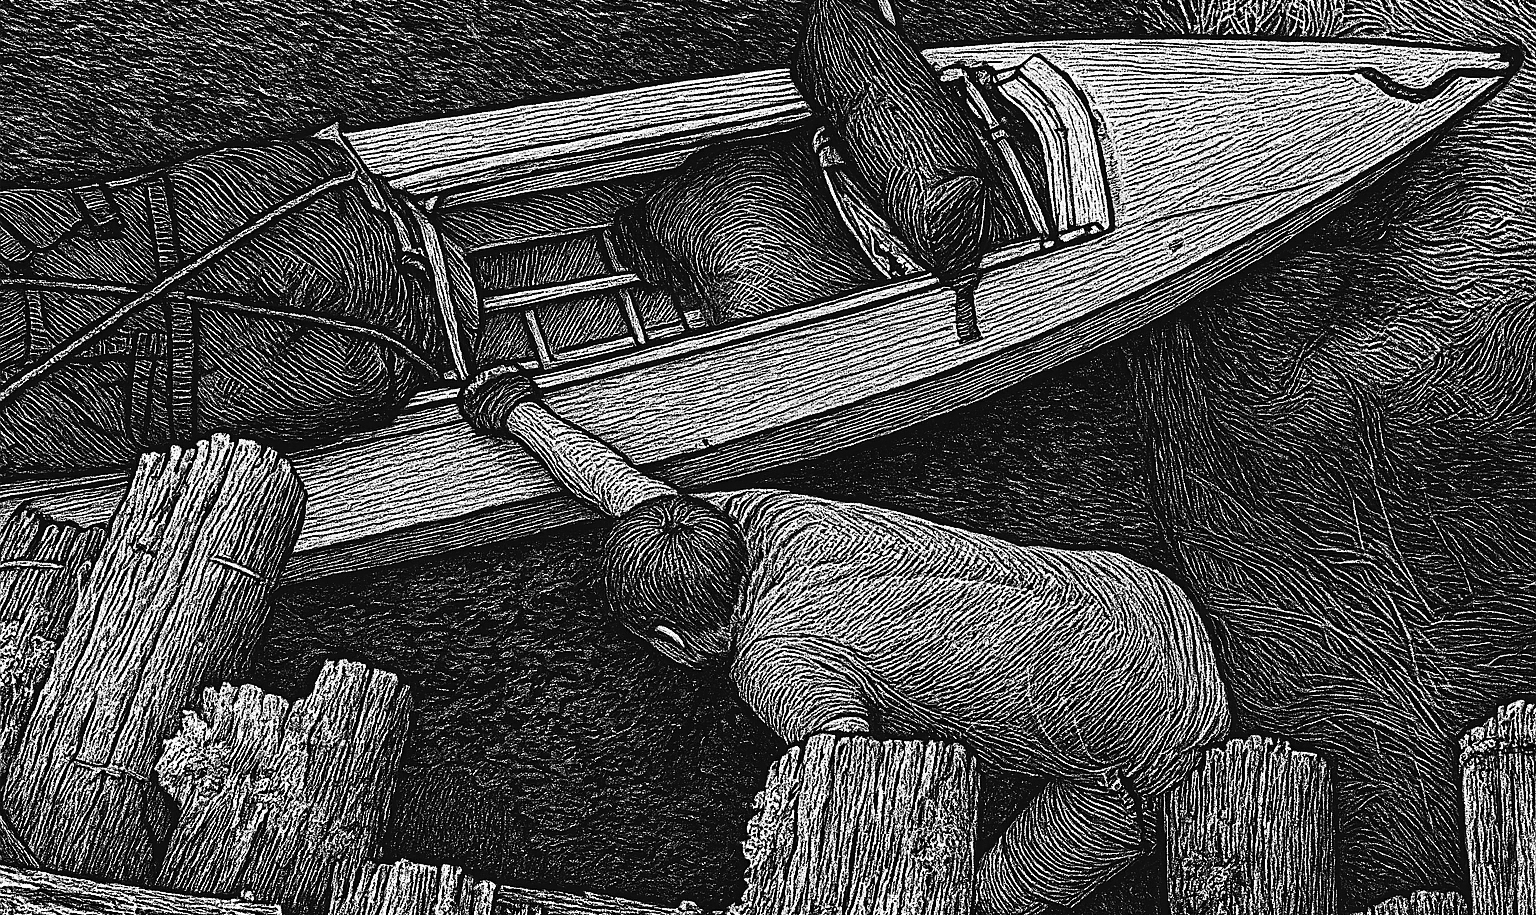
\includegraphics[width=1.0\textwidth]{22_serega}
	\caption{\small\textit{...Э-Э-Э!!!\mdash только и успел проорать Серёга...}}
\end{figure}

%----------------------------------------------------------------
\newpage

\begin{figure}[h]
	\centering
	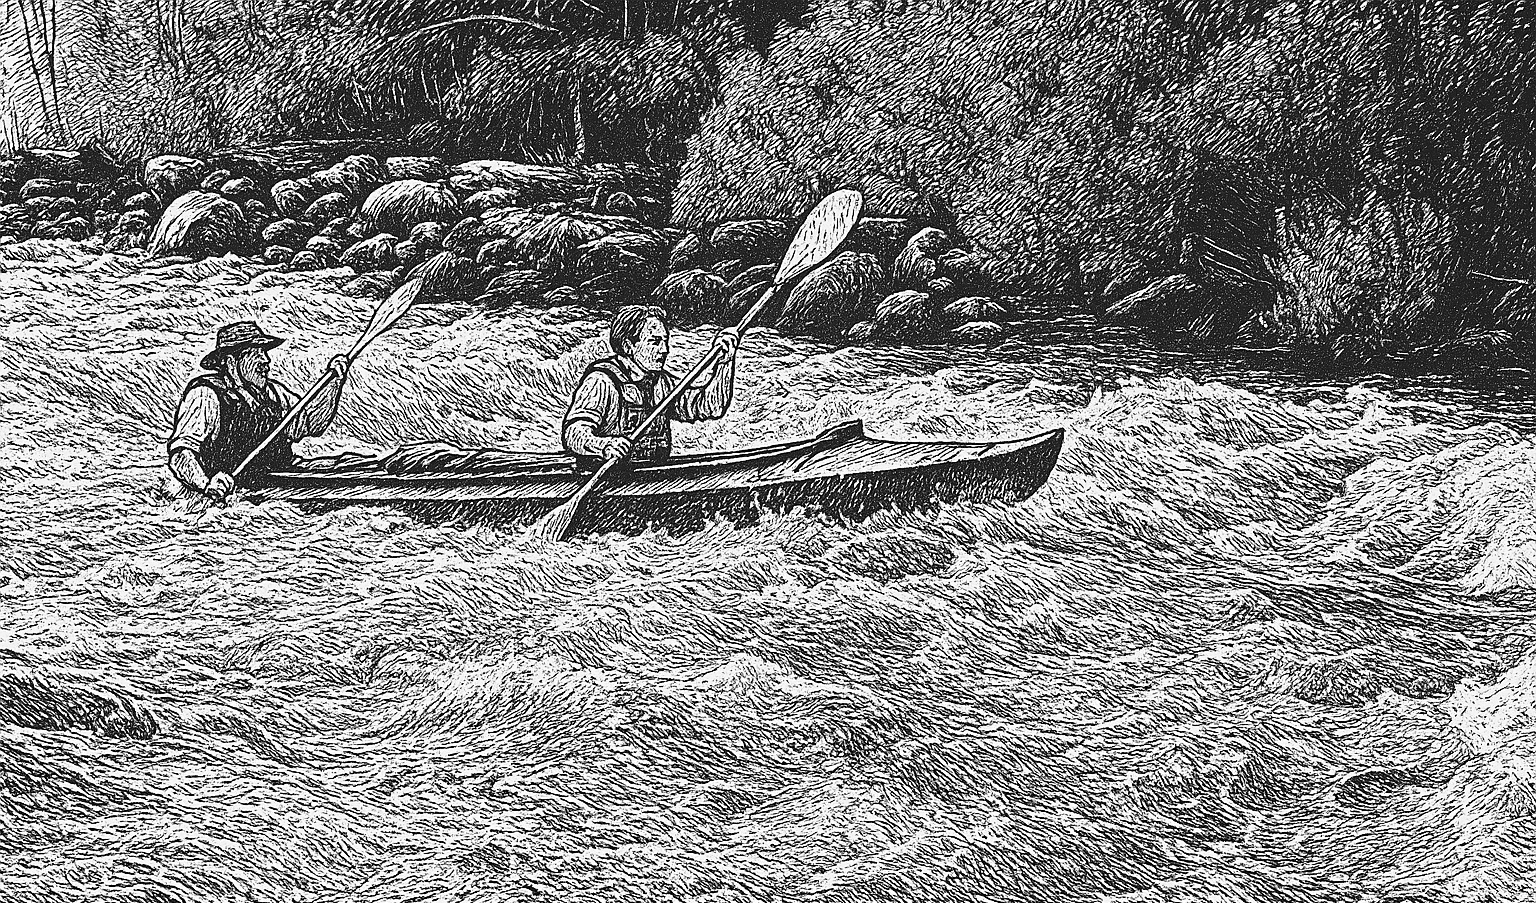
\includegraphics[width=1.0\textwidth]{23_fail}
	\caption{\small\textit{...Серёга!!! Левым!!!\mdash заорал Замполит...}}
\end{figure}

%----------------------------------------------------------------
\newpage

\begin{figure}[h]
	\centering
	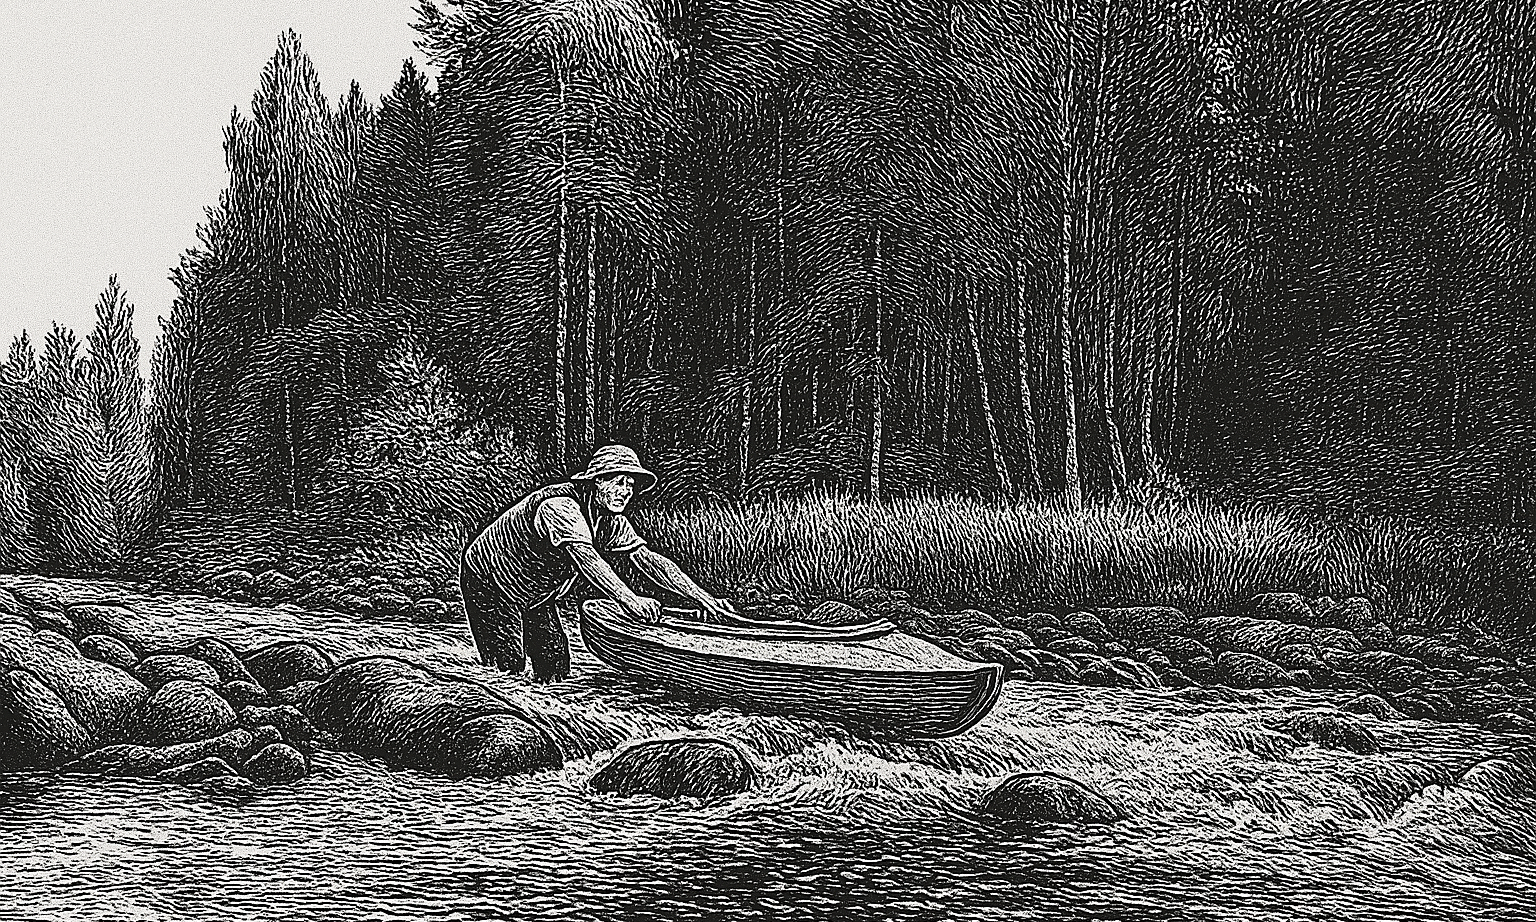
\includegraphics[width=1.0\textwidth]{24_nurmis}
	\caption{\small\textit{...пошли проводиться...}}
\end{figure}

%----------------------------------------------------------------
\newpage

\begin{figure}[h]
	\centering
	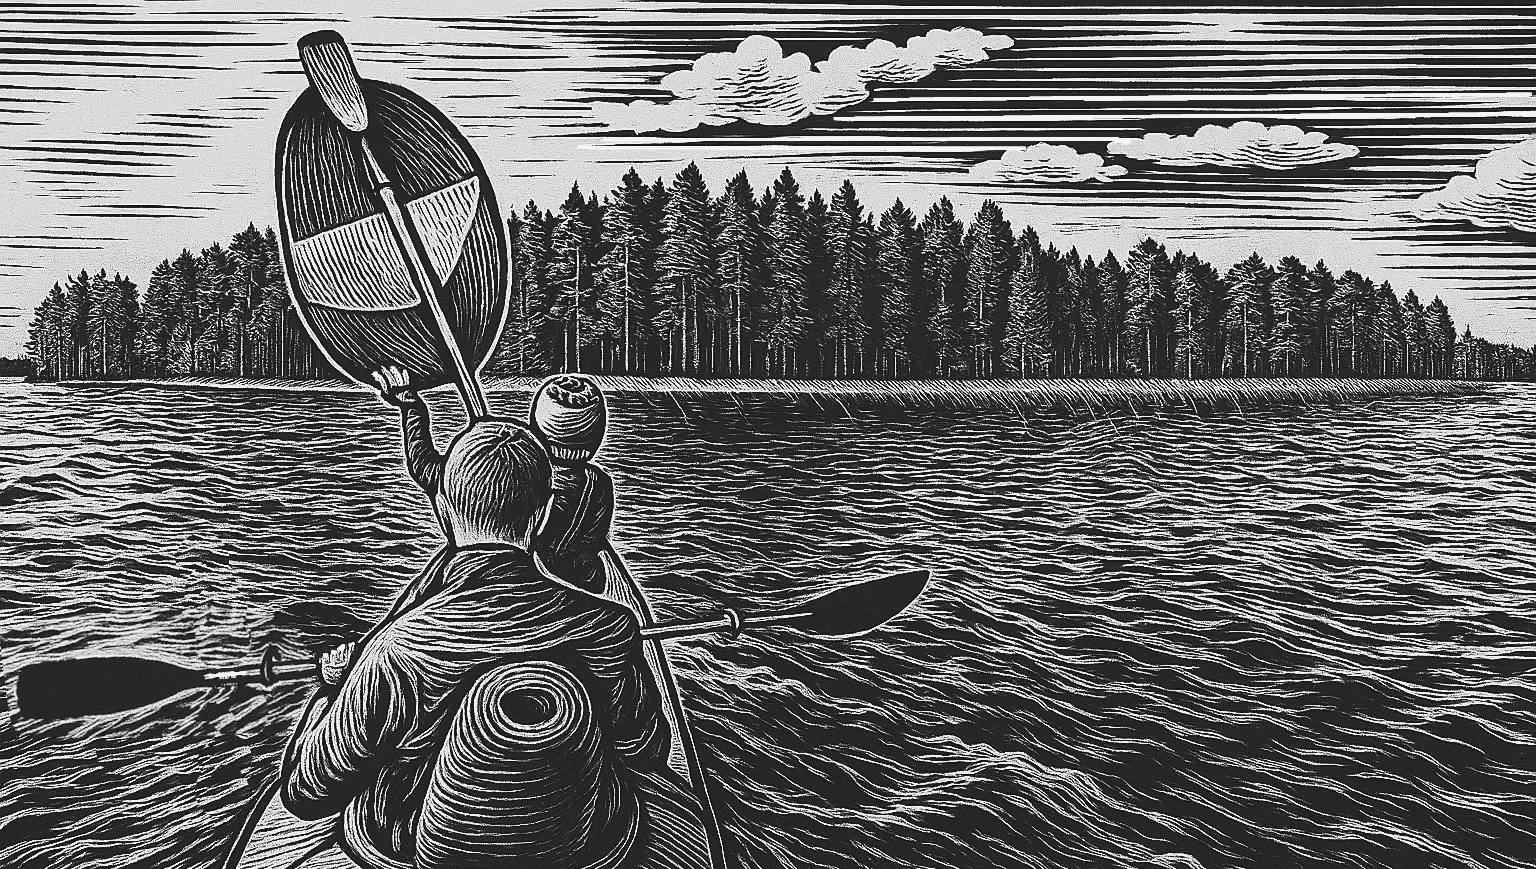
\includegraphics[width=1.0\textwidth]{25_island}
	\caption{\small\textit{...Ветер стремительно тащил их вперёд к острову...}}
\end{figure}

%----------------------------------------------------------------
\newpage

\begin{wrapfigure}[23]{l}{0.6\textwidth}
	%\begin{figure}[h]
	\centering
	\includegraphics[width=0.6\textwidth]{26_valkyrie}
	\caption{\small\textit{...завернувшись в одно полотенце...}}
	%\end{figure}
\end{wrapfigure}

\diagdash Дьявол, да хар{\'о}ш уже!!!\mdash Адмирал начал грести по\sdash активнее, чтобы справиться с~нахлынувшим.

\diagdash Шурик, куда ты так гребёшь?%Дай насладиться\sdash то, ну?

\diagdash Стоянку на днёвку ищем, или мне это снится?\mdash огрызнулся Адмирал.

\diagdash Ишь ты!\mdash Киря подрезал его на повороте,\mdash Хопа!\mdash и вышел вперёд.

\diagdash В заливчике давайте поглядим!\mdash Адмирал жадно вглядывался в~берег, они обогнули южный мыс и~зашли в~небольшую бухту.

%----------------------------------------------------------------
\newpage

\begin{wrapfigure}[23]{l}{0.6\textwidth}
	%\begin{figure}[h]
	\centering
	\includegraphics[width=0.6\textwidth]{27_shurik}
	\caption{\small\textit{...под сосной на берегу озера...}}
	%\end{figure}
\end{wrapfigure}

Вечер сгущался тёмный и~облачный. 
Над столом парни натянули тент, а к~соснам, росшим тут же, привалили гермы с продуктами и~вещмешки. 
%\begin{wrapfigure}[15]{l}{0.6\textwidth}
%\begin{figure}[h]
%	\centering
%	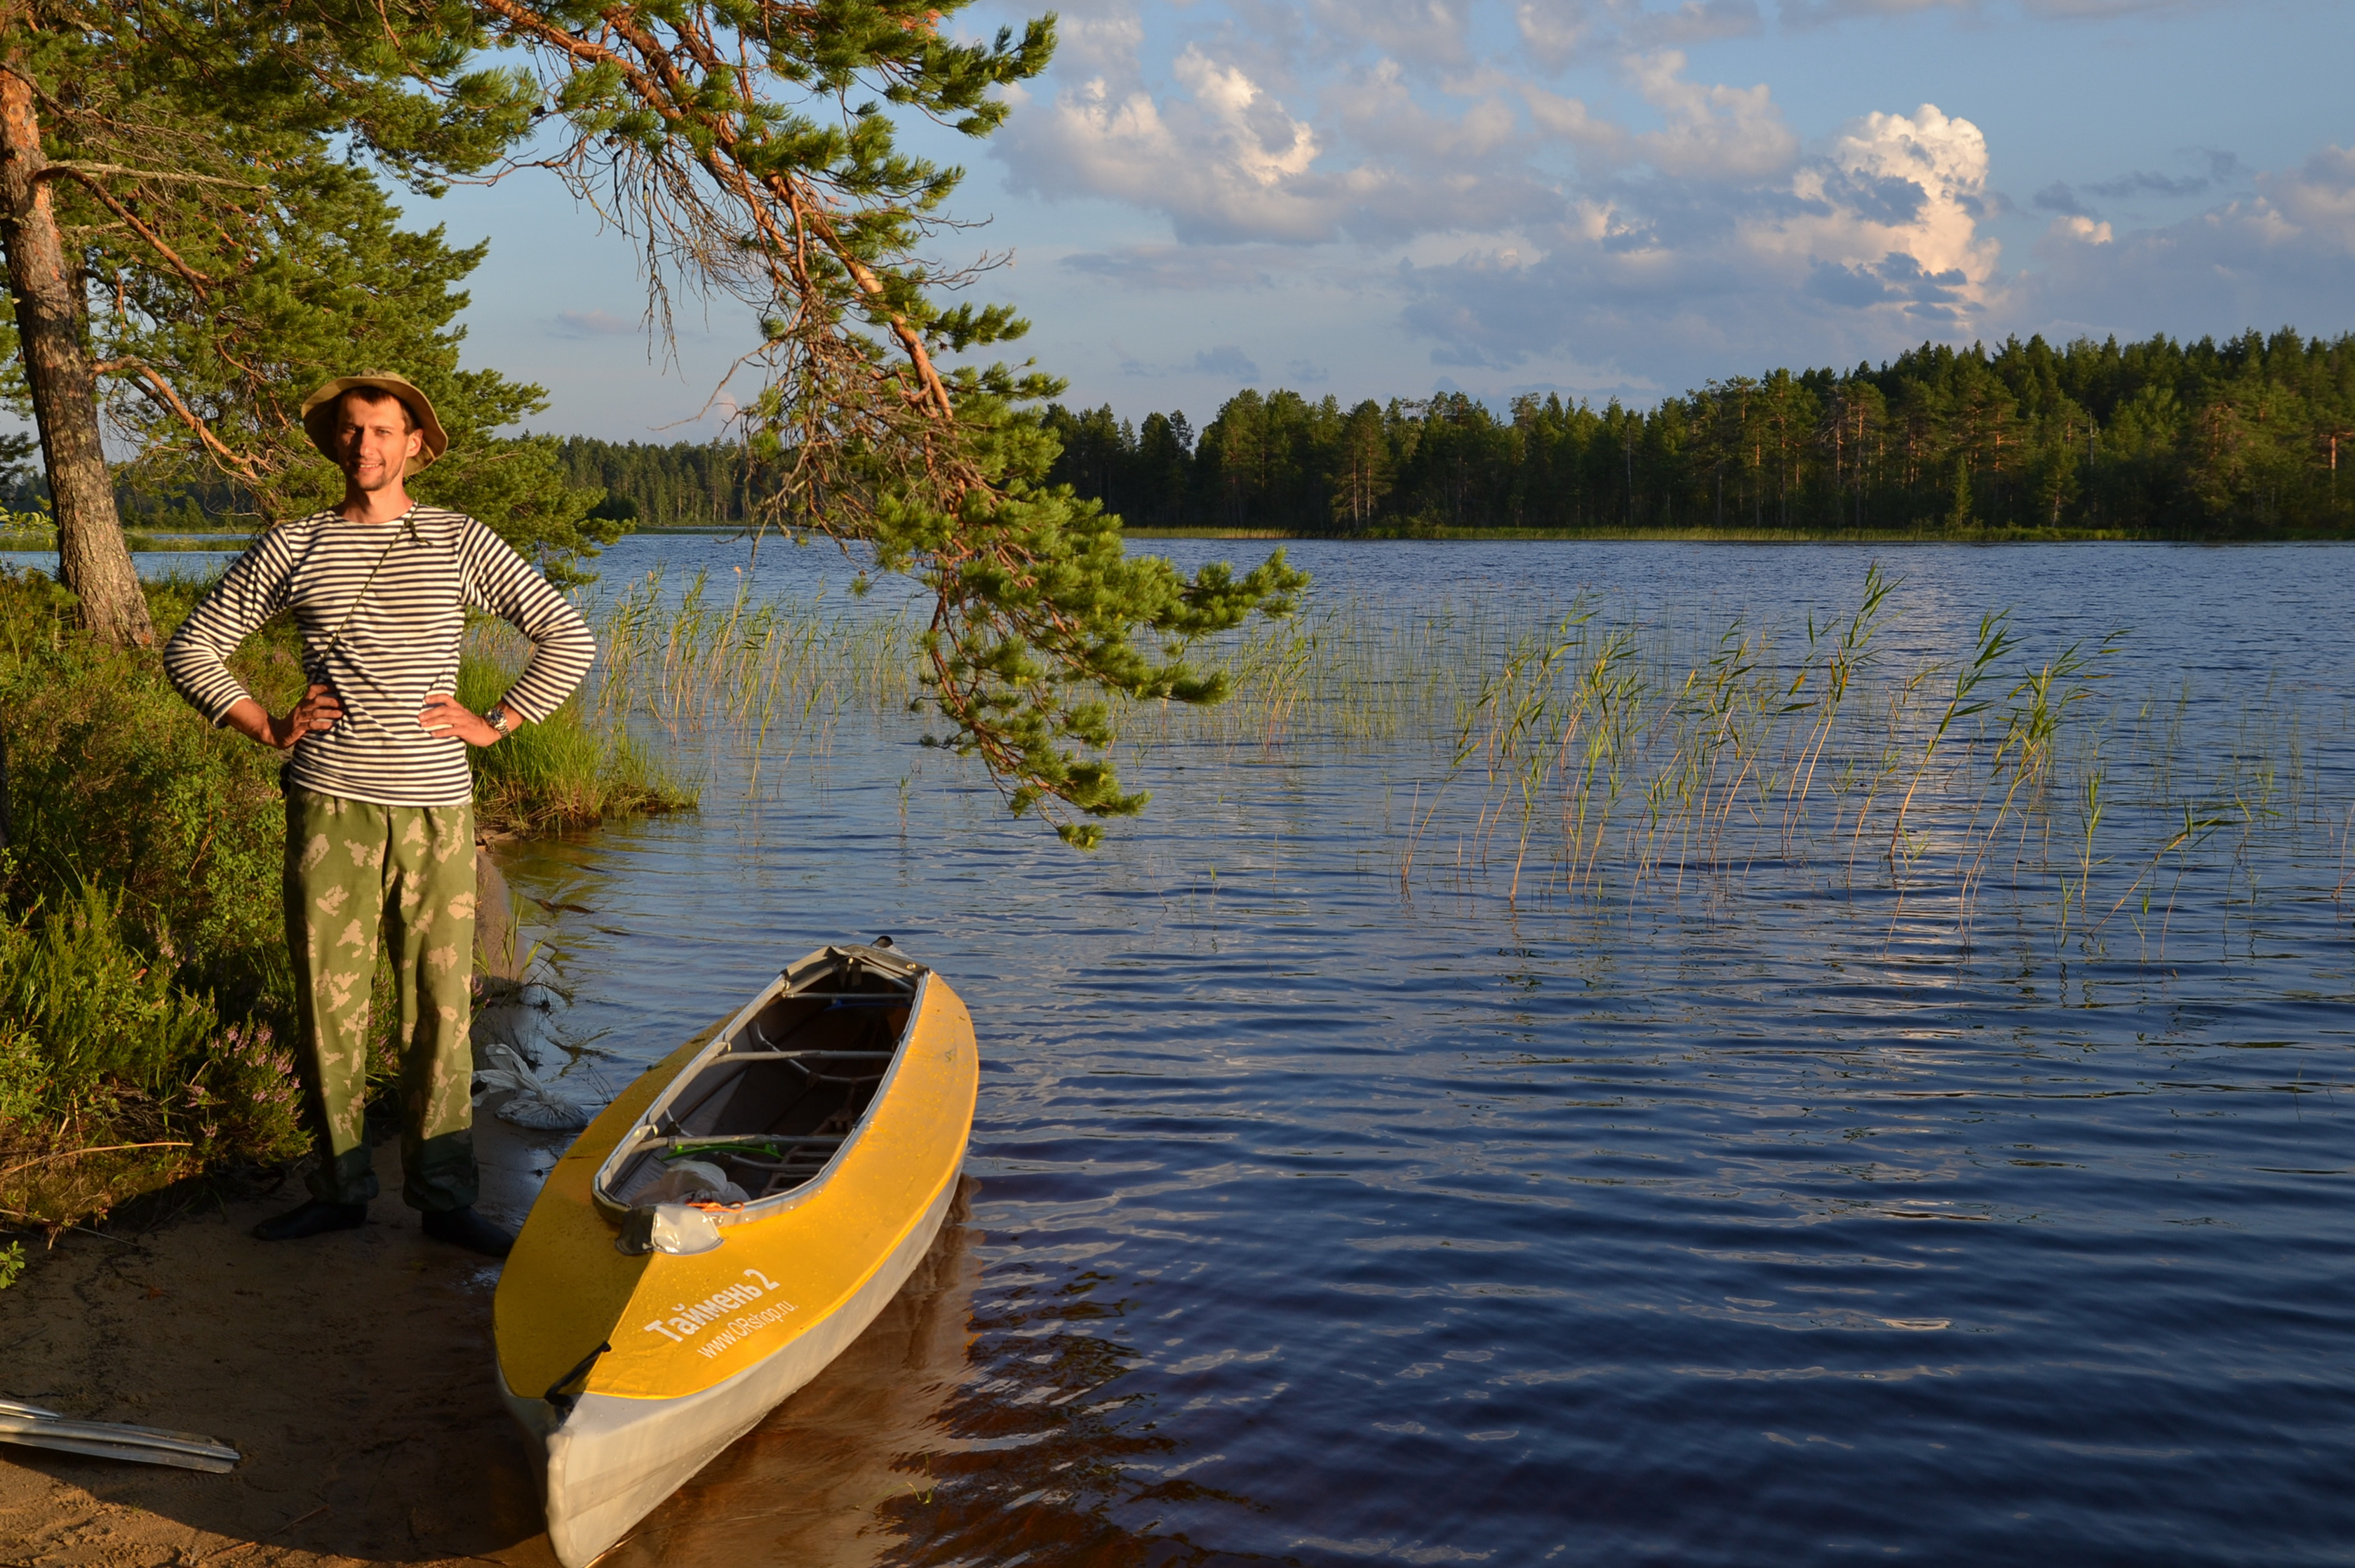
\includegraphics[width=1.0\textwidth]{9_4}
%	\caption{\small\textit{...пристали к берегу под сосной, росшей прям на берегу...}}
%\end{figure}
%\end{wrapfigure}
Костёр Адмирал мигом сообразил из имевшегося неподалёку валежника и отослал команду за нормальными дровами\mdash ему хотелось побыстрее сварить горячего.

Замполит~живо возглавил заготовку дров, дело спорилось\mdash у костра образовалась целая груда брёвен, что ребята притащили из леса. Котелки с водой уже пошумливали над костром, а Адмирал собрал свои походные кресла, уселся в~одно из них и распотрошил герму с~продуктами:

%----------------------------------------------------------------
% 10 ГЛАВА
%----------------------------------------------------------------
\newpage

\begin{figure}[h]
	\centering
	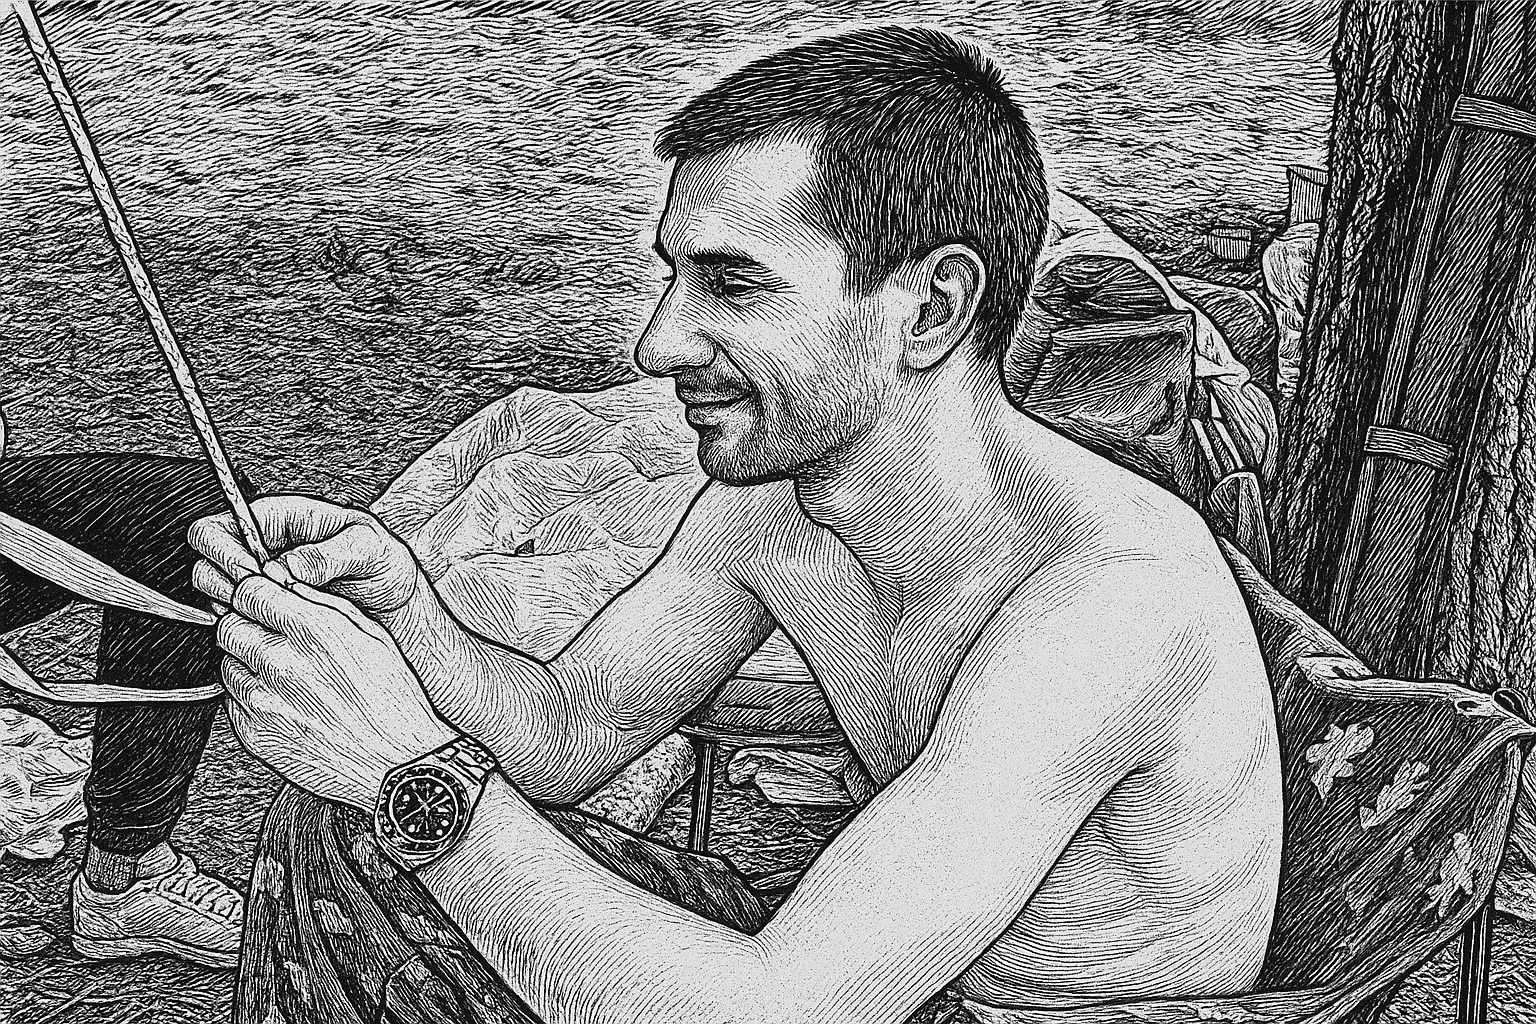
\includegraphics[width=1.0\textwidth]{28_chalka}
	\caption{\small\textit{...из этой ленты можно сплести чалку...}}
\end{figure}

%----------------------------------------------------------------
\newpage

\begin{figure}[h]
	\centering
	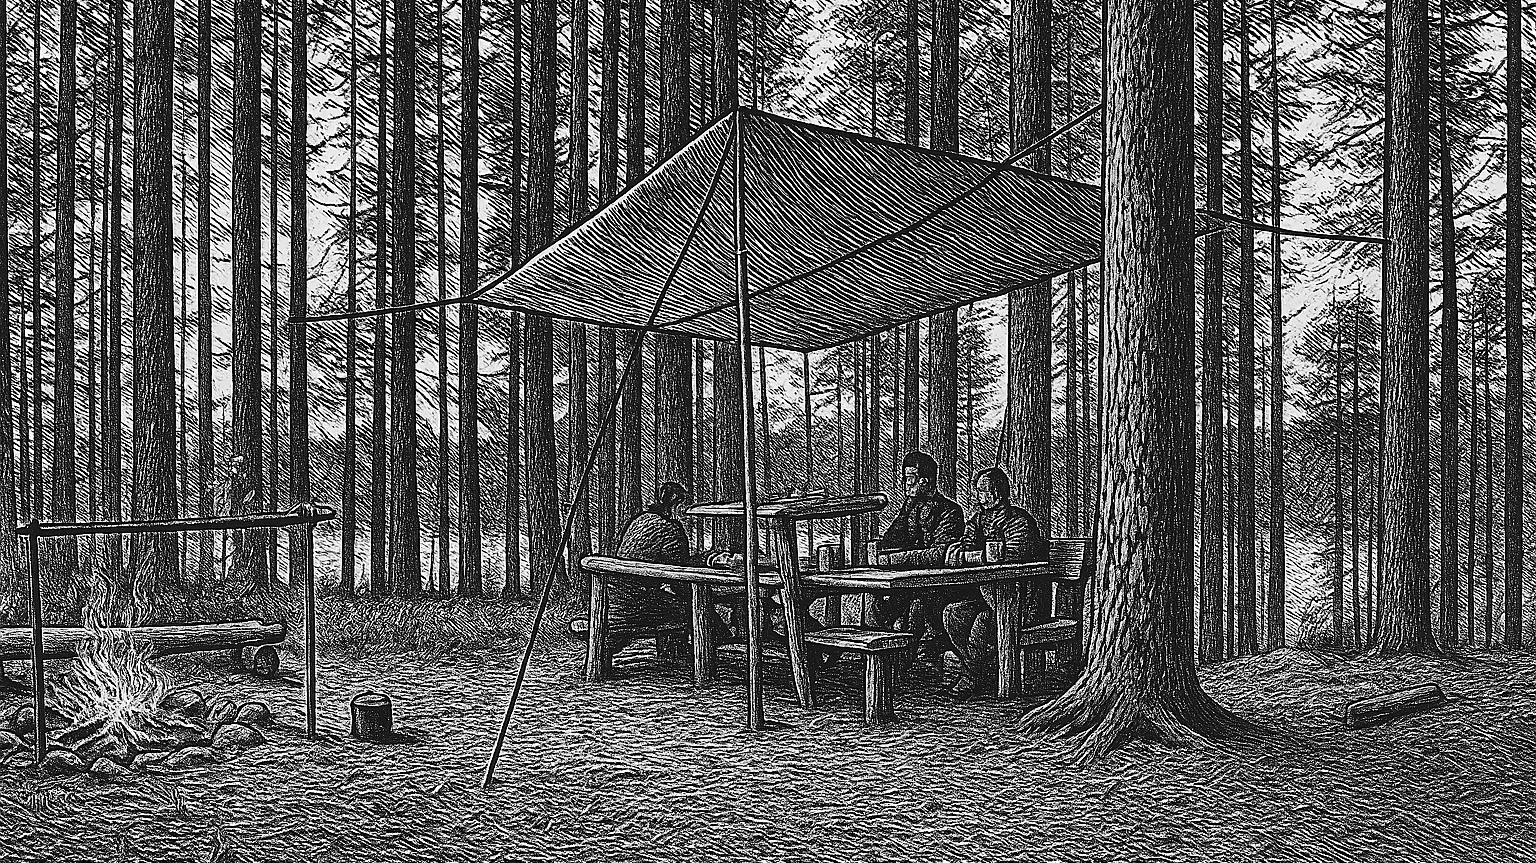
\includegraphics[width=1.0\textwidth]{29_tent}
	\caption{\small\textit{...в ослабший за ночь тент над~столом стала набираться вода...}}
\end{figure}

%----------------------------------------------------------------
\newpage

\begin{wrapfigure}[10]{r}{0.55\textwidth}
	%\begin{figure}[h]
	\centering
	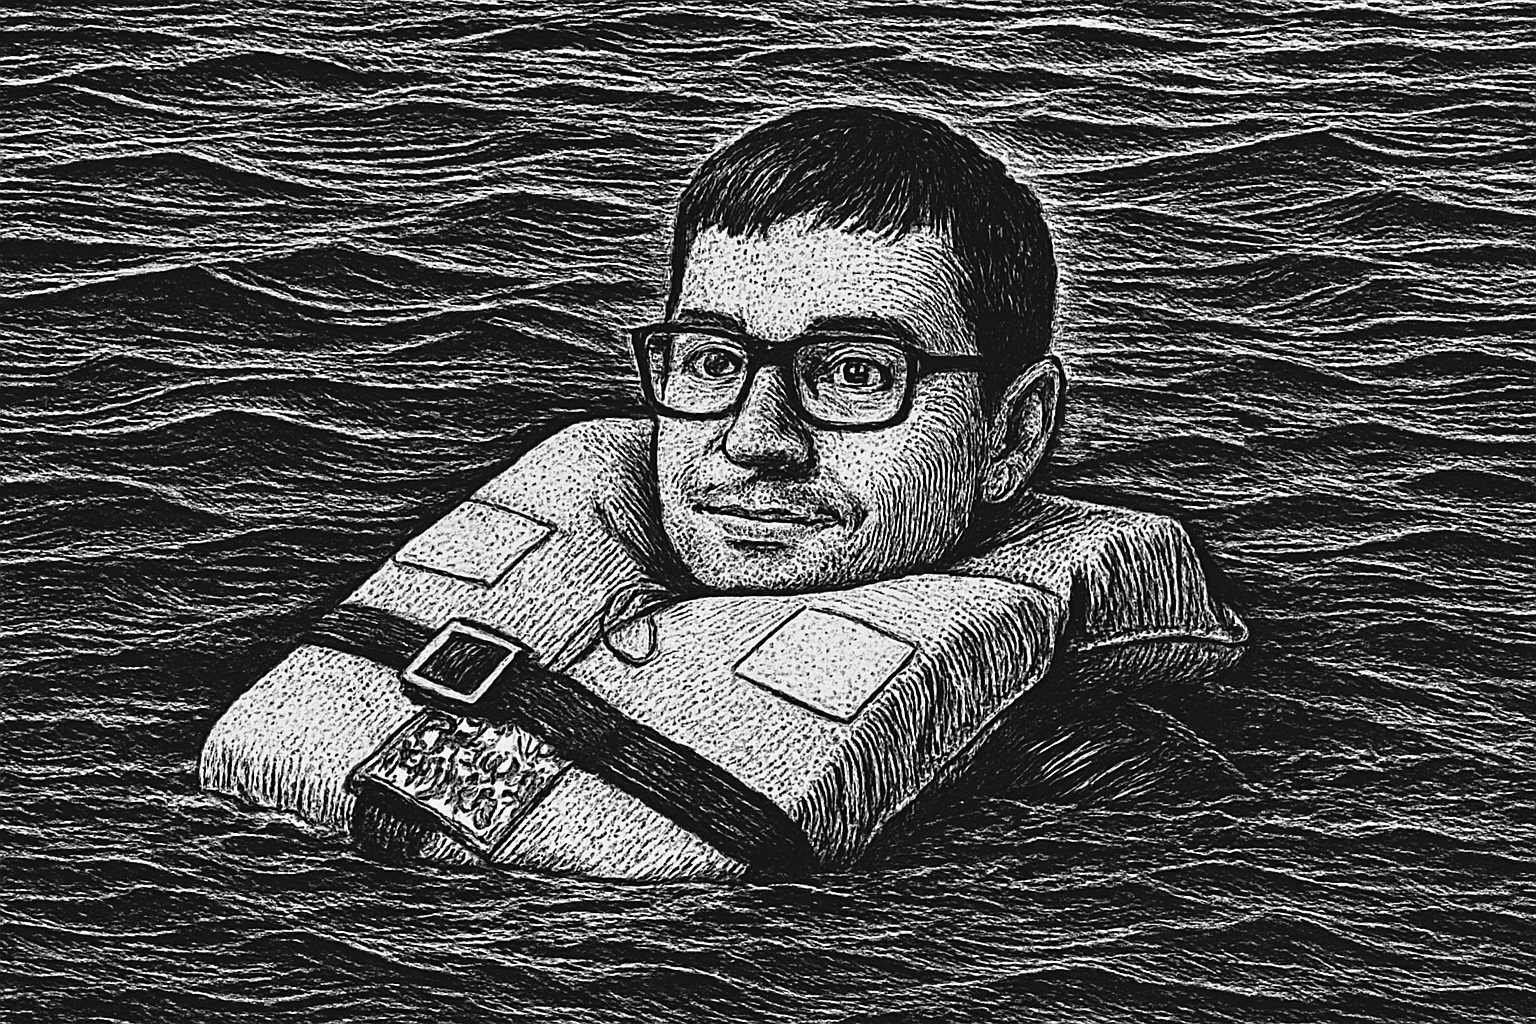
\includegraphics[width=0.5\textwidth]{30_lifejacket}
	\caption{\small\textit{...испытал свой спасжилет...}}
	%\end{figure}
\end{wrapfigure}испытал свой спасжилет и~успокоился. Руслан с~Пашей тусили под тентом, приканчивая красненькое:

\diagdash С бутылками что делать будем с пустыми? Не круто после себя стекло оставлять. Эх, молодо\sdash зелено, кто ж в~стекле с собой тащит?\mdash Паша разлил последнее.

%----------------------------------------------------------------
% 11 ГЛАВА
%----------------------------------------------------------------
\newpage

\begin{wrapfigure}[12]{l}{0.50\textwidth}
	%\begin{figure}[h]
	\centering
	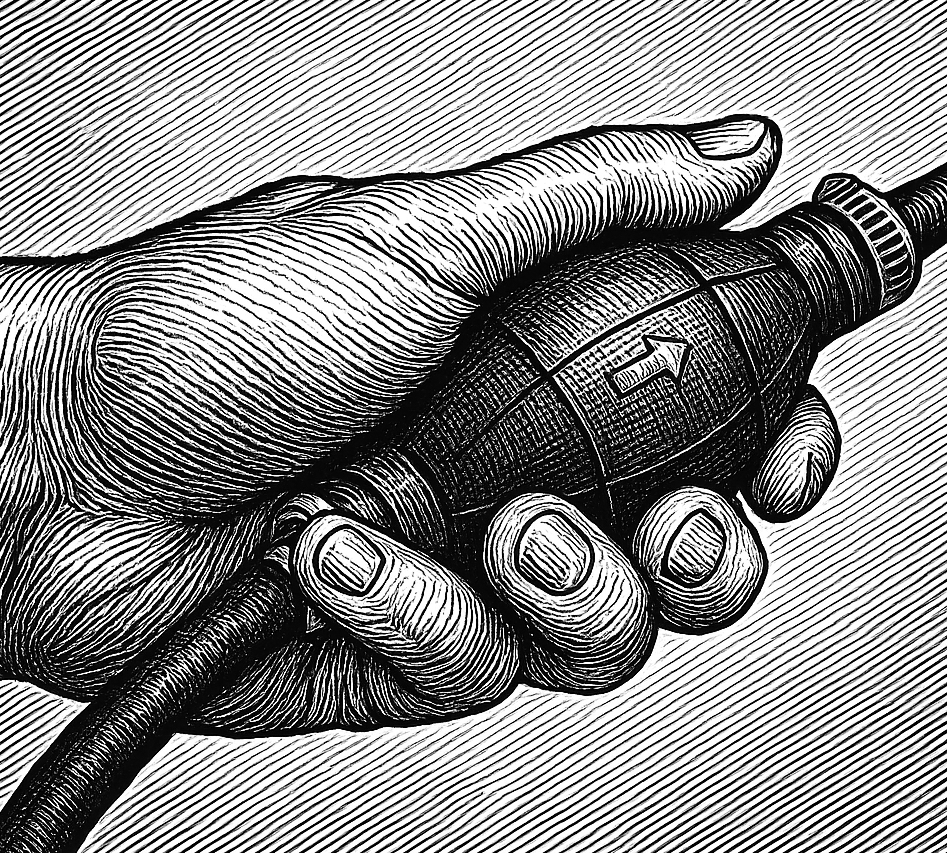
\includegraphics[width=0.5\textwidth]{31_pardon}
	\caption{\small\textit{...где моя, пардон...}}
	%\end{figure}
\end{wrapfigure}раз зажал и разжал грушу, отчего клапан в ней издал чавкающе\sdash булькающий звук.

\diagdash Ы-ы-ы! 

\diagdash Ну как\sdash то так, парни!\mdash Адмирал ещё раз проверил берег на~предмет забытых вещей и велел всем садиться в~байды.\mdash Пока мы собой и байдарочными юбками не~закроем проёмы, байды так и будет непрерывно заливать дождём!

%----------------------------------------------------------------
\newpage

\begin{figure}[h]
	\centering
	\includegraphics[width=1.0\textwidth]{32_bridge}
	\caption{\small\textit{...Вместо каких\sdash то пролётов лежало всего пару досок...}}
\end{figure}

%----------------------------------------------------------------
\newpage

\begin{figure}[h]
	\centering
	\includegraphics[width=1.0\textwidth]{33_porog}
	\caption{\small\textit{...Шум Уйтуженкоски...}}
\end{figure}

%----------------------------------------------------------------
\newpage

\begin{figure}[h]
	\centering
	\includegraphics[width=1.0\textwidth]{34_shturm}
	\caption{\small\textit{...УПЁРЛИСЬ ЖЁСТКО ПО~ЛЕВОМУ!!!...}}
\end{figure}

%----------------------------------------------------------------
\newpage

\begin{figure}[h]
	\centering	
	\includegraphics[width=1.0\textwidth]{35_otmel}
	\caption{\small\textit{...пошёл по каменистой гряде против течения...}}
\end{figure}

%----------------------------------------------------------------
\newpage

\begin{figure}[h]
	\centering
	\includegraphics[width=1.0\textwidth]{36_1_zampolit}
	\caption{\small\textit{...Замполит как раз жёстко выгребал поворот...}}
\end{figure}

%----------------------------------------------------------------
\newpage

\begin{wrapfigure}[12]{r}{0.48\textwidth}
	%\begin{figure}[h]
	\centering
	\includegraphics[width=0.46\textwidth]{37_radio}
	\caption{\small\textit{...спокуха, рация сдохла...}}
	%\end{figure}
\end{wrapfigure}

\diagdash Кнопку жмёшь и всё, экран гаснет, на.\mdash передал ему прибор Замполит.

\diagdash Ты её, засранец, позавчера не вырубил,\mdash догадался Адмирал.\mdash она у~тебя всю днёвку включённая была, сто процентов, вот аккумулятор и~сел в~ноль!!!

\diagdash Так ты не сказал$\ldots$

Адмирал уже набрал полные лёгкие разразиться матерной тирадой, но~удержался и только сказал, выдохнув:

%----------------------------------------------------------------
\newpage

\begin{figure}[h]
	\centering
	\includegraphics[width=1.0\textwidth]{38_suhoi}
	\caption{\small\textit{...ребята увидали выход из~порога...}}
\end{figure}

%----------------------------------------------------------------
\newpage

\begin{wrapfigure}[17]{r}{0.5\textwidth}
	%\begin{figure}[h]
	\centering
	\includegraphics[width=0.46\textwidth]{39_rum}
	\caption{\small\textit{...чай, лимон, всё харашо!...}}
	%\end{figure}
\end{wrapfigure}
\diagdash Можно уже, да?

\diagdash А то!

\diagdash Итак, мужики!\mdash начал Адмирал, пародируя акцент.\mdash Там шумит порог Каданлоама! Мы стоим тут на~островэ! У нас есть$\ldots$\mdash он посмотрел в кружку, полную кубинского рома,\mdash $\ldots$чай, лимон, всё харашо! Да? Мы~переоделись в сухоэ, одэжда у нас вон там на вэрёвочке сушится висит! Кирь, засними эту выставку\sdash продажу! Вон~там всё сушится!$\ldots$


\diagdash После героического прохождения порогов!\mdash вставил Паша.

%----------------------------------------------------------------
\newpage

\begin{figure}[h]
	\centering
	\includegraphics[width=1.0\textwidth]{40_fire}
	\caption{\small\textit{...у пылающего костра...}}
\end{figure}


%----------------------------------------------------------------
\newpage

\begin{figure}[h]
	\centering
	\includegraphics[width=1.0\textwidth]{41_pikefish}
	\caption{\small\textit{...ещё и щука под вечер...}}
\end{figure}

%----------------------------------------------------------------
\newpage

\begin{figure}[h]
	\centering
	\includegraphics[width=1.0\textwidth]{42_1_cigar}
	\caption{\small\textit{...вечер проходил у них с ленцой...}}
\end{figure}

%----------------------------------------------------------------
\newpage

\begin{figure}[h]
	\centering
	%	\includegraphics[width=1.0\textwidth]{11_5}
	\includegraphics[width=1.0\textwidth]{43_cheranga}
	\caption{\small\textit{...Адмирал сходил к берегу пофотографировать разлив Черанги...}}
\end{figure}

%----------------------------------------------------------------
% 12 ГЛАВА
%----------------------------------------------------------------
\newpage

\begin{wrapfigure}[12]{l}{0.48\textwidth}
	%\begin{figure}[h]
	\centering
	\includegraphics[width=0.45\textwidth]{44_porridge}
	\caption{\small\textit{...пшёнка с изюмом...}}
	%\end{figure}
\end{wrapfigure}
\diagdash Сань, чё у нас сегодня?\mdash Паша покончил с~кашей и~достал конфеты к~чаю.

\diagdash Вчера обсуждали вродь как. Сегодня\mdash ещё 4 порога последних и дальше по широкой Суне почти до~Викшозера. Кирь, доставай описание порогов\mdash самое время освежить в~памяти.
%----------------------------------------------------------------
\newpage

\begin{figure}[h]
	\centering
	\includegraphics[width=1.0\textwidth]{45_bochka}
	\caption{\small\textit{...рубанули байдаркой прямо по плите...}}
\end{figure}

%----------------------------------------------------------------
\newpage

\begin{figure}[h]
	\centering
	\includegraphics[width=1.0\textwidth]{46_endporogs}
	\caption{\small\textit{...пороги кончились...}}
\end{figure}

%----------------------------------------------------------------
\newpage

\begin{wrapfigure}[13]{l}{0.5\textwidth}
	%\begin{figure}[h]
	\centering
	\includegraphics[width=0.47\textwidth]{47_coffee}
	\caption{\small\textit{...я вам кофеёк обещал...}}
	%\end{figure}
\end{wrapfigure}
Адмирал выполз из~палатки. Дождь почти закончился, но~погодка оставляла желать лучшего\mdash лес вокруг был влажным, дул неслабый ветерочек. Он~распалил костёр из~напиленных вчера впрок дров, поставил воду в~котелке на~чай\mdash всё равно кто\sdash нибудь да захочет чай\mdash и~принялся за кофе. Немного подумав, решил варить кофе на~газу, а~не~на~костре. Для этого он достал и собрал свою мини\sdash горелку, собрал защитный экранчик от ветра, поставил десантный котелок на синий цветок газа, щедро насыпал молотый кофе. Сверху он закрыл котелок подкотельником\mdash получилась как бы крышка\mdash так быстрее закипело. Народ потихонку стал подтягиваться к костру.

%----------------------------------------------------------------
\newpage

\begin{wrapfigure}[20]{r}{0.58\textwidth}
	%\begin{figure}[h]
	\centering
	\includegraphics[width=0.56\textwidth]{48_pancakes}
	\caption{\small\textit{...принялся за оладьи...}}
	%\end{figure}
\end{wrapfigure}
\diagdash Шурик, такого ты ещё не делал.\mdash изрёк подошедший Замполит, тоже соблазнившись на~кофе.

\diagdash Не, помнишь, мы когда в последний раз по Чагодоще ходили, тоже кофеёк варили как\sdash то?

\diagdash А, тот наш <<арктический>> поход? Смутно~уже.

\diagdash Варили\sdash варили, было дело.\mdash подтвердил Серёга.

\diagdash Ну вот я решил повторить, так сказать.\mdash Адмирал вполне насладился напитком и принялся за оладьи. Он~достал из продуктовой гермы блинную муку и стал читать инструкцию на упаковке.


%----------------------------------------------------------------
\newpage

\begin{wrapfigure}[10]{r}{0.5\textwidth}
	%\begin{figure}[h]
	\centering
	\includegraphics[width=0.48\textwidth]{49_kompot}
	\caption{\small\textit{...компотика наварить?...}}
	%\end{figure}
\end{wrapfigure}

Спустя совсем немного времени компот был готов:

\diagdash Нава-а-аристо!

\diagdash А то!

\diagdash Серёга у нас главный по компотам в~этом сплаве.\mdash попробовал компот Руслан.

\diagdash Не, по компотикам главный\mdash Замполит, а Серёга по сборке голубики.\mdash не преминул подколоть Замполита Адмирал.

%----------------------------------------------------------------
\newpage

\begin{wrapfigure}[22]{l}{0.58\textwidth}
	%\begin{figure}[h]
	\centering
	\includegraphics[width=0.56\textwidth]{50_fishsmoke}
	\caption{\small\textit{...Паша стал снимать рыбу...}}
	%\end{figure}
\end{wrapfigure}
ываооывшоа ываы ывщшао ывашгор ываг вргш ывар вышгфр рывы горгшр ш щш щш шщг щшгщшг  гшны ы ываооывшоа ываы ывщшао ывашгор ываг вргш ывар вышгфр рывы горгшр ш щш щш шщг щшгщшг  гшны ы ываооывшоа ываы ывщшао ывашгор ываг вргш ывар вышгфр рывы горгшр ш щш щш шщг щшгщшг  гшны ы ываооывшоа ываы ывщшао ывашгор ываг вргш ывар вышгфр рывы горгшр ш щш щш шщг щшгщшг  гшны ы ываооывшоа ываы ывщшао ывашгор ываг вргш ывар вышгфр рывы горгшр ш щш щш шщг щшгщшг  гшны ы ываооывшоа ываы ывщшао ывашгор ываг вргш ывар вышгфр рывы горгшр ш щш щш шщг щшгщшг  гшны ы ываооывшоа ываы ывщшао ывашгор ываг вргш ывар вышгфр рывы горгшр 

ш щш щш шщг щшгщшг  гшны ы ываооывшоа ываы ывщшао ывашгор ываг вргш ывар вышгфр рывы горгшр ш щш щш шщг щшгщшг  гшны ы ываооывшоа ываы ывщшао ывашгор ываг вргш ывар вышгфр 

%----------------------------------------------------------------
\newpage

\begin{wrapfigure}[11]{l}{0.58\textwidth}
	%\begin{figure}[h]
	\centering
	\includegraphics[width=0.56\textwidth]{51_mushrooms}
	\caption{\small\textit{...зажарили лисички...}}
	%\end{figure}
\end{wrapfigure}
ывар вышгфр рывы горгшр ш щш щш шщг щшгщшг  гшны ы ываооывшоа ываы ывщшао ывашгор ываг вргш ывар вышгфр рывы горгшр ш щш щш шщг щшгщшг  гшны ы ываооывшоа ываы ывщшао ывашгор ываг вргш ывар вышгфр рывы горгшр ш щш щш шщг щшгщшг  гшны ы ываооывшоа ываы ывщшао 

ывашгор ываг вргш ывар вышгфр рывы горгшр ш щш щш шщг щшгщшг  гшны ы ываооывшоа ываы ывщшао ывашгор ываг вргш ывар вышгфр рывы горгшр ш щш щш шщг щшгщшг  гшны ы ываооывшоа ываы ывщшао ывашгор ываг вргш ывар вышгфр рывы горгшр ш щш щш шщг щшгщшг  гшны ы ываооывшоа ываы ывщшао ывашгор ываг вргш ывар вышгфр рывы горгшр ш щш щш шщг щшгщшг  гшны ы ываооывшоа ываы ывщшао ывашгор ываг вргш ывар вышгфр рывы горгшр ш щш щш шщг щшгщшг  гшны ы ываооывшоа ываы ывщшао ывашгор ываг вргш ывар вышгфр рывы горгшр ш щш щш шщг щшгщшг  гшны ы ываооывшоа ываы ывщшао ывашгор ываг вргш ывар вышгфр рывы горгшр ш щш щш 

%----------------------------------------------------------------
\newpage

\begin{wrapfigure}[12]{l}{0.58\textwidth}
	%\begin{figure}[h]
	\centering
	\includegraphics[width=0.56\textwidth]{52_delight}
	\caption{\small\textit{...Адмирал закрыл глаза...}}
	%\end{figure}
\end{wrapfigure}
шщг щшгщшг  гшны ы ываооывшоа ываы ывщшао ывашгор ываг вргш ывар вышгфр рывы горгшр ш щш щш шщг щшгщшг  гшны ы ываооывшоа ываы ывщшао ывашгор ываг вргш ывар вышгфр рывы горгшр ш щш щш шщг щшгщшг  гшны ы ываооывшоа ываы ывщшао ывашгор ываг вргш ывар вышгфр рывы горгшр ш щш щш шщг щшгщшг  гшны ы ываооывшоа ываы ывщшао ывашгор ываг вргш ывар вышгфр рывы горгшр ш щш щш шщг щшгщшг  гшны ы ываооывшоа ываы ывщшао ывашгор ываг вргш ывар вышгфр рывы горгшр ш щш щш шщг щшгщшг  гшны ы ываооывшоа ываы ывщшао ывашгор ываг вргш ывар вышгфр рывы горгшр ш щш щш шщг щшгщшг  гшны ы ываооывшоа ываы ывщшао ывашгор ываг вргш ывар вышгфр рывы горгшр ш щш щш шщг щшгщшг  гшны ы ываооывшоа ываы ывщшао ывашгор ываг вргш ывар вышгфр рывы горгшр ш щш щш шщг щшгщшг  гшны ы ываооывшоа ываы ывщшао ывашгор ываг вргш ывар вышгфр рывы горгшр ш щш щш шщг щшгщшг  гшны ы 




 % Дорога домой
\chapter{Тест2}

Тестовая глава для печати всех иллюстраций.

\newpage

%----------------------------------------------------------------
% 1 ГЛАВА
%----------------------------------------------------------------


\begin{figure}[h]
	\centering
	\includegraphics[width=1.0\textwidth]{01_train}
	\caption{\small\textit{...в электричке c Курского вокзала...}}	
\end{figure}

%----------------------------------------------------------------
% 2 ГЛАВА
%----------------------------------------------------------------

\newpage

Сеструха, тем временем, задорно отплясывала в центре зала, широко улыбаясь, светя забитой татухой рукой и~оголёнными плечами, справедливо упиваясь торжеством молодости, красоты, задора. Светлые завитые локоны подплясывали в такт движениям, вишнёвое вечернее платье подчёркивало все её сочные достоинства.

\noindent
\begin{minipage}{0.48\textwidth}
	\setlength{\parindent}{1.0cm}  % Включаем красную строку
	
	\indent \diagdash Пошли~потанцуем?\mdash вдруг жарко шепнула жена на~ухо Шурику.
	
	\indent \diagdash А пошли!\mdash он приобнял жену и закружил в толпе танцующих гостей, словно желая выкружить все крамольные мысли из~головы$\ldots$
	
	\indent $\ldots$Стол ломился, друзья широко, разгульно праздновали:
	
	\indent \diagdash Дорогие Кирилл и~Надежда$\ldots$\mdash полились речи, всё как обычно, ничего нового. От этих речей Шурику вдруг стало невообразимо скучно, да~так, что свело скулы.
\end{minipage}\hfill
\begin{minipage}{0.5\textwidth}
	\centering
	\includegraphics[width=\linewidth]{02_wedding}
	
	{\small\textit{...в платье белом...}}
\end{minipage}

%----------------------------------------------------------------
% 3 ГЛАВА
%----------------------------------------------------------------
\newpage

\begin{figure}[h]
	\centering
	\includegraphics[width=1.0\textwidth]{03_1_beer}
	\caption{\small\textit{...Адмирал с Замполитом сидели в пивнушке...}}
\end{figure}

%----------------------------------------------------------------
\newpage

\noindent
\begin{minipage}{0.55\textwidth}
	\setlength{\parindent}{1.0cm}  % Включаем красную строку
	\setlength{\parskip}{0.25cm}     % Межабзацный отступ, как в основном тексте
	
	\noindent байдарочных фартука, надев их на себя. Узнал издалека, не~ошиблась.
	
	\diagdash Так, вот, держите,\mdash стала передавать, снимая с~себя снарягу, байдарочница, а~Шурик стал навешивать фартуки и~жилеты уже на~себя.
	
	\diagdash А остальное?	
	
	\diagdash А остальное на другом складе, надо пройти минут пять, пошли?\mdash маняще мотнула она головой в~сторону 9\sdash этажек и~поправила волосы$\ldots$
\end{minipage}\hfill
\begin{minipage}{0.40\textwidth}
	\centering
	\includegraphics[width=\linewidth]{04_1_girl}
	
	{\small\textit{...с~хитрым~прищуром...}}
\end{minipage}

%----------------------------------------------------------------
\newpage

\begin{wrapfigure}[11]{l}{0.49\textwidth}
	%\begin{figure}[h]
	\centering
	%	\includegraphics[width=1.0\textwidth]{3_new3}
	\includegraphics[width=0.47\textwidth]{05_1_map}
	\caption{\small\textit{...повело плёнку...}}
	%\end{figure}
\end{wrapfigure}

\diagdash А~дубликат~есть?\mdash заволновалась Надя.

\diagdash Нет уж, пойдём по такой карте.\mdash Замполит деланно закатил глаза.\mdash Потеряемся, как пить дать! Ё\sdash моё! Ну всё, Шурик, по~такой карте идти нельзя! 

\diagdash Всё пропало, Кирь!\mdash подыграл тот.


%----------------------------------------------------------------
% 4 ГЛАВА
%----------------------------------------------------------------

%\newpage
\vspace{20mm}

\begin{figure}[h]
	\centering
	\includegraphics[width=1.0\textwidth]{06_1_highway}
	\caption{\small\textit{...бодро рванул вперёд по автостраде, утапливая педаль газа...}}
\end{figure}

%----------------------------------------------------------------
% 5 ГЛАВА
%----------------------------------------------------------------
\newpage

\begin{figure}[h]
	\centering
	\includegraphics[width=1.0\textwidth]{07_ladoga}
	\caption{\small\textit{...нет, не скифы, не азиаты мы...}}
\end{figure}

%----------------------------------------------------------------
\newpage

text text

\noindent
\begin{minipage}{0.45\textwidth}
	\setlength{\parindent}{1.0cm}  % Восстановление отступа абзаца
	
	\indent Смотровая площадка располагалась после 4-й ступени водопада, самой высокой, а~немного выше был виден предыдущий каскад с~двумя чуть меньшими водопадиками. Друзья забрались в~самый дальний край тропинки на~гору, где была установлена лавочка и~открывался чудесный вид вниз на~долину. Присели на лавочку передохнуть и~подождать Серёгу с~Русланом.
	
	\indent Кивач\mdash жемчужина Карелии. Заповедник был \makebox[\linewidth][s]{\noindent создан в~30\sdash ые годы XX\hspace{0.25em}в.}
\end{minipage}\hfill
\begin{minipage}{0.5\textwidth}
	\centering
	\includegraphics[width=\linewidth]{08_kivach}
	
	{\small\textit{...жемчужина Карелии...}}
\end{minipage}

%----------------------------------------------------------------
\newpage

\begin{figure}[h]
	\centering
	\includegraphics[width=1.0\textwidth]{09_2_ussr}
	\caption{\small\textit{...молоткасто-серпастое...}}
\end{figure}

%----------------------------------------------------------------
% 6 ГЛАВА
%----------------------------------------------------------------
\newpage

\begin{figure}[h]
	\centering
	\includegraphics[width=1.0\textwidth]{10_1_jeep}
	\caption{\small\textit{...свернули направо на Нёлгомозеро...}}
\end{figure}

abcd

\begin{figure}[h]
	\centering
	\includegraphics[width=1.0\textwidth]{11_1_keelson}
	\caption{\small\textit{...фальшборт не лезет...}}
\end{figure}

%----------------------------------------------------------------
\newpage

\begin{figure}[h]
	\centering
	\includegraphics[width=1.0\textwidth]{12_1_maybe}
	\caption{\small\textit{...А чё, давайте может?...}}
\end{figure}

abcd

\newpage

\begin{wrapfigure}[10]{l}{0.52\textwidth}
	\setlength{\belowcaptionskip}{-10pt}
	%	\begin{figure}[h]
		\centering
		\includegraphics[width=0.52\textwidth]{13_skol}
		\caption{\small\textit{...два отрывистых...}}
		%	\end{figure}
\end{wrapfigure}

\noindent И сегодня нас ждут каналы между озёрами ещё, кстати. Итак, то, к~чему мы стремились\mdash свершается! Мы выбрались в наш первый совместный сплав по Карелии и, надеюсь, это приключение запомнится нам надолго! Ну,~мужики, будем!\mdash лес рук с кружками поднялся и замер, ожидая команды.\mdash Тащ~Замполит, два отрывистых и одно раскатистое!!!

%----------------------------------------------------------------
% 7 ГЛАВА
%----------------------------------------------------------------
\newpage

\begin{figure}[h]
	\centering
	\includegraphics[width=1.0\textwidth]{14_channel}
	\caption{\small\textit{...Канал был шириной примерно метров 8...}}
\end{figure}

%----------------------------------------------------------------
\newpage

\begin{figure}[h]
	\centering
	\includegraphics[width=1.0\textwidth]{15_1_okular}
	\caption{\small\textit{...ты говорил, что у тебя подзорная труба есть?...}}
\end{figure}

%----------------------------------------------------------------
% 8 ГЛАВА
%----------------------------------------------------------------
\newpage

\noindent
\begin{minipage}{0.38\textwidth}
	\setlength{\parindent}{1.0cm}  % Включаем красную строку
	\setlength{\parskip}{0.25cm}     % Межабзацный отступ, как в основном тексте
	
	\vspace{-0.4cm}
	\diagdash И\sdash и\sdash иха! 
	
	\diagdash ПОТАЩИЛО!!! --- Адмирал в полном восторге перестал грести веслом по\sdash байдарочному и~взял его под мышку на манер руля.\mdash Погнали!!!
	
	Ветер дул, конечно, не~особо сильный, но этого было вполне достаточно, чтобы дать им ход в~парочку км/ч. Второй экипаж, тем временем, наконец\sdash то отчалил и~догнал их:
\end{minipage}\hfill
\begin{minipage}{0.57\textwidth}
	\centering
	\includegraphics[width=0.95\linewidth]{16_1_parus}
	
	{\small\textit{...ветер стал усиливаться...}}
\end{minipage}

%----------------------------------------------------------------
\newpage

\begin{wrapfigure}[20]{r}{0.55\textwidth}
	%\begin{figure}[h]
	\centering
	\includegraphics[width=0.55\textwidth]{17_2_tree}
	\caption{\small\textit{...Мы нашли Иггдрасиль!...}}
	%\end{figure}
\end{wrapfigure}
\diagdash Ваще похоже$\ldots$

\diagdash Шурик, там это, ясень был, у~скандинавов.\mdash сказал подошедший Киря.

\diagdash А у нас сосна будет! Она роднее как\sdash то. Мне всегда нравилась такая мифология\mdash древнегреческая и~древнеримская, потом древнескандинавская$\ldots$ Красиво они всё расписывали, черти!

\diagdash Да ты язычник?

\diagdash Это церковники христианские очернить чтобы придумали\mdash язычники, язычники, тьфу! У меня настольная книга была в школе\mdash <<Легенды и мифы Древней Греции и~Древнего Рима>>\cite{Кун}. Потом на~Скандинавию переключился$\ldots$ Красиво же!

%----------------------------------------------------------------
\newpage

\begin{figure}[h]
	\centering
	\includegraphics[width=1.0\textwidth]{18_mountain}
	\caption{\small\textit{...На~горизонте виднелась гора Ундойвара...}}
\end{figure}

\begin{wrapfigure}[11]{r}{0.45\textwidth}
	%\begin{figure}[h]
	\centering
	\includegraphics[width=0.45\textwidth]{19_1_blueberry}
	\caption{\small\textit{...Полный котелок черники...}}
	%\end{figure}
\end{wrapfigure}

%----------------------------------------------------------------
\newpage

\diagdash Не, парни, только троекратное <<УРА>> или <<SKÅL>>!\mdash Адмирал взял дольку апельсинчика.

%\diagdash Не, парни, только расово\sdash чистое троекратное <<УРА>> или <<SKÅL>>!\mdash Адмирал взял апельсинчик.

\diagdash Пофиг, будем!\mdash лес железных кубков поднялся.

\diagdash Кампай!

\diagdash SKÅL! Ну тебя с этим <<кампаем>>! Давай компотик варить!\mdash Адмирал попробовал спелую чернику.

%----------------------------------------------------------------
\newpage

\begin{figure}[h]
	\centering
	\includegraphics[width=1.0\textwidth]{20_1_fish}
	\caption{\small\textit{...А что там с супом?...}}
\end{figure}

%----------------------------------------------------------------
\newpage

\begin{figure}[h]
	\centering
	\includegraphics[width=1.0\textwidth]{21_moon.png}
	\caption{\small\textit{...Луна, взошедшая над лесом, отражалась в Мярандуксе...}}
\end{figure}

%----------------------------------------------------------------
% 9 ГЛАВА
%----------------------------------------------------------------
\newpage

\begin{figure}[h]
	\centering
	\includegraphics[width=1.0\textwidth]{22_1_serega}
	\caption{\small\textit{...Э-Э-Э!!!\mdash только и успел проорать Серёга...}}
\end{figure}

%----------------------------------------------------------------
\newpage

\begin{figure}[h]
	\centering
	\includegraphics[width=1.0\textwidth]{23_1_fail}
	\caption{\small\textit{...Серёга!!! Левым!!!\mdash заорал Замполит...}}
\end{figure}

%----------------------------------------------------------------
\newpage

\begin{figure}[h]
	\centering
	\includegraphics[width=1.0\textwidth]{24_1_nurmis}
	\caption{\small\textit{...пошли проводиться...}}
\end{figure}

%----------------------------------------------------------------
\newpage

\begin{figure}[h]
	\centering
	\includegraphics[width=1.0\textwidth]{25_1_island}
	\caption{\small\textit{...Ветер стремительно тащил их вперёд к острову...}}
\end{figure}

%----------------------------------------------------------------
\newpage

\begin{wrapfigure}[23]{l}{0.6\textwidth}
	%\begin{figure}[h]
	\centering
	\includegraphics[width=0.6\textwidth]{26_4_valkyrie}
	\caption{\small\textit{...завернувшись в одно полотенце...}}
	%\end{figure}
\end{wrapfigure}

\diagdash Дьявол, да хар{\'о}ш уже!!!\mdash Адмирал начал грести по\sdash активнее, чтобы справиться с~нахлынувшим.

\diagdash Шурик, куда ты так гребёшь?%Дай насладиться\sdash то, ну?

\diagdash Стоянку на днёвку ищем, или мне это снится?\mdash огрызнулся Адмирал.

\diagdash Ишь ты!\mdash Киря подрезал его на повороте,\mdash Хопа!\mdash и вышел вперёд.

\diagdash В заливчике давайте поглядим!\mdash Адмирал жадно вглядывался в~берег, они обогнули южный мыс и~зашли в~небольшую бухту.

%----------------------------------------------------------------
\newpage

\begin{wrapfigure}[23]{l}{0.6\textwidth}
	%\begin{figure}[h]
	\centering
	\includegraphics[width=0.6\textwidth]{27_1_shurik}
	\caption{\small\textit{...под сосной на берегу озера...}}
	%\end{figure}
\end{wrapfigure}

Вечер сгущался тёмный и~облачный. 
Над столом парни натянули тент, а к~соснам, росшим тут же, привалили гермы с продуктами и~вещмешки. 
%\begin{wrapfigure}[15]{l}{0.6\textwidth}
%\begin{figure}[h]
%	\centering
%	\includegraphics[width=1.0\textwidth]{9_4}
%	\caption{\small\textit{...пристали к берегу под сосной, росшей прям на берегу...}}
%\end{figure}
%\end{wrapfigure}
Костёр Адмирал мигом сообразил из имевшегося неподалёку валежника и отослал команду за нормальными дровами\mdash ему хотелось побыстрее сварить горячего.

Замполит~живо возглавил заготовку дров, дело спорилось\mdash у костра образовалась целая груда брёвен, что ребята притащили из леса. Котелки с водой уже пошумливали над костром, а Адмирал собрал свои походные кресла, уселся в~одно из них и распотрошил герму с~продуктами:

%----------------------------------------------------------------
% 10 ГЛАВА
%----------------------------------------------------------------
\newpage

\begin{figure}[h]
	\centering
	\includegraphics[width=1.0\textwidth]{28_1_chalka}
	\caption{\small\textit{...из этой ленты можно сплести чалку...}}
\end{figure}

%----------------------------------------------------------------
\newpage

\begin{figure}[h]
	\centering
	\includegraphics[width=1.0\textwidth]{29_1_tent}
	\caption{\small\textit{...в ослабший за ночь тент над~столом стала набираться вода...}}
\end{figure}

%----------------------------------------------------------------
\newpage

\begin{wrapfigure}[10]{r}{0.55\textwidth}
	%\begin{figure}[h]
	\centering
	\includegraphics[width=0.5\textwidth]{30_1_lifejacket}
	\caption{\small\textit{...испытал свой спасжилет...}}
	%\end{figure}
\end{wrapfigure}испытал свой спасжилет и~успокоился. Руслан с~Пашей тусили под тентом, приканчивая красненькое:

\diagdash С бутылками что делать будем с пустыми? Не круто после себя стекло оставлять. Эх, молодо\sdash зелено, кто ж в~стекле с собой тащит?\mdash Паша разлил последнее.

%----------------------------------------------------------------
% 11 ГЛАВА
%----------------------------------------------------------------
\newpage

\begin{wrapfigure}[12]{l}{0.50\textwidth}
	%\begin{figure}[h]
	\centering
	\includegraphics[width=0.5\textwidth]{31_pardon}
	\caption{\small\textit{...где моя, пардон...}}
	%\end{figure}
\end{wrapfigure}раз зажал и разжал грушу, отчего клапан в ней издал чавкающе\sdash булькающий звук.

\diagdash Ы-ы-ы! 

\diagdash Ну как\sdash то так, парни!\mdash Адмирал ещё раз проверил берег на~предмет забытых вещей и велел всем садиться в~байды.\mdash Пока мы собой и байдарочными юбками не~закроем проёмы, байды так и будет непрерывно заливать дождём!

%----------------------------------------------------------------
\newpage

\begin{figure}[h]
	\centering
	\includegraphics[width=1.0\textwidth]{32_1_bridge}
	\caption{\small\textit{...Вместо каких\sdash то пролётов лежало всего пару досок...}}
\end{figure}

%----------------------------------------------------------------
\newpage

\begin{figure}[h]
	\centering
	\includegraphics[width=1.0\textwidth]{33_1_porog}
	\caption{\small\textit{...Шум Уйтуженкоски...}}
\end{figure}

%----------------------------------------------------------------
\newpage

\begin{figure}[h]
	\centering
	\includegraphics[width=1.0\textwidth]{34_1_shturm}
	\caption{\small\textit{...УПЁРЛИСЬ ЖЁСТКО ПО~ЛЕВОМУ!!!...}}
\end{figure}

%----------------------------------------------------------------
\newpage

\begin{figure}[h]
	\centering	
	\includegraphics[width=1.0\textwidth]{35_1_otmel}
	\caption{\small\textit{...пошёл по каменистой гряде против течения...}}
\end{figure}

%----------------------------------------------------------------
\newpage

\begin{figure}[h]
	\centering
	\includegraphics[width=1.0\textwidth]{36_3_zampolit}
	\caption{\small\textit{...Замполит как раз жёстко выгребал поворот...}}
\end{figure}

%----------------------------------------------------------------
\newpage

\begin{wrapfigure}[12]{r}{0.48\textwidth}
	%\begin{figure}[h]
	\centering
	\includegraphics[width=0.46\textwidth]{37_1_radio}
	\caption{\small\textit{...спокуха, рация сдохла...}}
	%\end{figure}
\end{wrapfigure}

\diagdash Кнопку жмёшь и всё, экран гаснет, на.\mdash передал ему прибор Замполит.

\diagdash Ты её, засранец, позавчера не вырубил,\mdash догадался Адмирал.\mdash она у~тебя всю днёвку включённая была, сто процентов, вот аккумулятор и~сел в~ноль!!!

\diagdash Так ты не сказал$\ldots$

Адмирал уже набрал полные лёгкие разразиться матерной тирадой, но~удержался и только сказал, выдохнув:

%----------------------------------------------------------------
\newpage

\begin{figure}[h]
	\centering
	\includegraphics[width=1.0\textwidth]{38_1_suhoi}
	\caption{\small\textit{...ребята увидали выход из~порога...}}
\end{figure}

%----------------------------------------------------------------
\newpage

\begin{wrapfigure}[17]{r}{0.5\textwidth}
	%\begin{figure}[h]
	\centering
	\includegraphics[width=0.46\textwidth]{39_2_rum}
	\caption{\small\textit{...чай, лимон, всё харашо!...}}
	%\end{figure}
\end{wrapfigure}
\diagdash Можно уже, да?

\diagdash А то!

\diagdash Итак, мужики!\mdash начал Адмирал, пародируя акцент.\mdash Там шумит порог Каданлоама! Мы стоим тут на~островэ! У нас есть$\ldots$\mdash он посмотрел в кружку, полную кубинского рома,\mdash $\ldots$чай, лимон, всё харашо! Да? Мы~переоделись в сухоэ, одэжда у нас вон там на вэрёвочке сушится висит! Кирь, засними эту выставку\sdash продажу! Вон~там всё сушится!$\ldots$


\diagdash После героического прохождения порогов!\mdash вставил Паша.

%----------------------------------------------------------------
\newpage

\begin{figure}[h]
	\centering
	\includegraphics[width=1.0\textwidth]{40_1_fire}
	\caption{\small\textit{...у пылающего костра...}}
\end{figure}


%----------------------------------------------------------------
\newpage

\begin{figure}[h]
	\centering
	\includegraphics[width=1.0\textwidth]{41_1_pikefish}
	\caption{\small\textit{...ещё и щука под вечер...}}
\end{figure}

%----------------------------------------------------------------
\newpage

\begin{figure}[h]
	\centering
	\includegraphics[width=1.0\textwidth]{42_3_cigar}
	\caption{\small\textit{...вечер проходил у них с ленцой...}}
\end{figure}

%----------------------------------------------------------------
\newpage

\begin{figure}[h]
	\centering
	%	\includegraphics[width=1.0\textwidth]{11_5}
	\includegraphics[width=1.0\textwidth]{43_1_cheranga}
	\caption{\small\textit{...Адмирал сходил к берегу пофотографировать разлив Черанги...}}
\end{figure}

%----------------------------------------------------------------
% 12 ГЛАВА
%----------------------------------------------------------------
\newpage

\begin{wrapfigure}[12]{l}{0.48\textwidth}
	%\begin{figure}[h]
	\centering
	\includegraphics[width=0.45\textwidth]{44_1_porridge}
	\caption{\small\textit{...пшёнка с изюмом...}}
	%\end{figure}
\end{wrapfigure}
\diagdash Сань, чё у нас сегодня?\mdash Паша покончил с~кашей и~достал конфеты к~чаю.

\diagdash Вчера обсуждали вродь как. Сегодня\mdash ещё 4 порога последних и дальше по широкой Суне почти до~Викшозера. Кирь, доставай описание порогов\mdash самое время освежить в~памяти.
%----------------------------------------------------------------
\newpage

\begin{figure}[h]
	\centering
	\includegraphics[width=1.0\textwidth]{45_1_bochka}
	\caption{\small\textit{...рубанули байдаркой прямо по плите...}}
\end{figure}

%----------------------------------------------------------------
\newpage

\begin{figure}[h]
	\centering
	\includegraphics[width=1.0\textwidth]{46_1_endporogs}
	\caption{\small\textit{...пороги кончились...}}
\end{figure}

%----------------------------------------------------------------
% 13 ГЛАВА
%----------------------------------------------------------------
\newpage

\begin{wrapfigure}[13]{l}{0.5\textwidth}
	%\begin{figure}[h]
	\centering
	\includegraphics[width=0.47\textwidth]{47_1_coffee}
	\caption{\small\textit{...я вам кофеёк обещал...}}
	%\end{figure}
\end{wrapfigure}
Адмирал выполз из~палатки. Дождь почти закончился, но~погодка оставляла желать лучшего\mdash лес вокруг был влажным, дул неслабый ветерочек. Он~распалил костёр из~напиленных вчера впрок дров, поставил воду в~котелке на~чай\mdash всё равно кто\sdash нибудь да захочет чай\mdash и~принялся за кофе. Немного подумав, решил варить кофе на~газу, а~не~на~костре. Для этого он достал и собрал свою мини\sdash горелку, собрал защитный экранчик от ветра, поставил десантный котелок на синий цветок газа, щедро насыпал молотый кофе. Сверху он закрыл котелок подкотельником\mdash получилась как бы крышка\mdash так быстрее закипело. Народ потихонку стал подтягиваться к костру.

%----------------------------------------------------------------
\newpage

\begin{wrapfigure}[20]{r}{0.58\textwidth}
	%\begin{figure}[h]
	\centering
	\includegraphics[width=0.56\textwidth]{48_1_pancakes}
	\caption{\small\textit{...принялся за оладьи...}}
	%\end{figure}
\end{wrapfigure}
\diagdash Шурик, такого ты ещё не делал.\mdash изрёк подошедший Замполит, тоже соблазнившись на~кофе.

\diagdash Не, помнишь, мы когда в последний раз по Чагодоще ходили, тоже кофеёк варили как\sdash то?

\diagdash А, тот наш <<арктический>> поход? Смутно~уже.

\diagdash Варили\sdash варили, было дело.\mdash подтвердил Серёга.

\diagdash Ну вот я решил повторить, так сказать.\mdash Адмирал вполне насладился напитком и принялся за оладьи. Он~достал из продуктовой гермы блинную муку и стал читать инструкцию на упаковке.


%----------------------------------------------------------------
\newpage

\begin{wrapfigure}[10]{r}{0.5\textwidth}
	%\begin{figure}[h]
	\centering
	\includegraphics[width=0.48\textwidth]{49_1_kompot}
	\caption{\small\textit{...компотика наварить?...}}
	%\end{figure}
\end{wrapfigure}

Спустя совсем немного времени компот был готов:

\diagdash Нава-а-аристо!

\diagdash А то!

\diagdash Серёга у нас главный по компотам в~этом сплаве.\mdash попробовал компот Руслан.

\diagdash Не, по компотикам главный\mdash Замполит, а Серёга по сборке голубики.\mdash не преминул подколоть Замполита Адмирал.

%----------------------------------------------------------------
\newpage

\begin{wrapfigure}[22]{l}{0.58\textwidth}
	%\begin{figure}[h]
	\centering
	\includegraphics[width=0.56\textwidth]{50_1_fishsmoke}
	\caption{\small\textit{...Паша стал снимать рыбу...}}
	%\end{figure}
\end{wrapfigure}
ываооывшоа ываы ывщшао ывашгор ываг вргш ывар вышгфр рывы горгшр ш щш щш шщг щшгщшг  гшны ы ываооывшоа ываы ывщшао ывашгор ываг вргш ывар вышгфр рывы горгшр ш щш щш шщг щшгщшг  гшны ы ываооывшоа ываы ывщшао ывашгор ываг вргш ывар вышгфр рывы горгшр ш щш щш шщг щшгщшг  гшны ы ываооывшоа ываы ывщшао ывашгор ываг вргш ывар вышгфр рывы горгшр ш щш щш шщг щшгщшг  гшны ы ываооывшоа ываы ывщшао ывашгор ываг вргш ывар вышгфр рывы горгшр ш щш щш шщг щшгщшг  гшны ы ываооывшоа ываы ывщшао ывашгор ываг вргш ывар вышгфр рывы горгшр ш щш щш шщг щшгщшг  гшны ы ываооывшоа ываы ывщшао ывашгор ываг вргш ывар вышгфр рывы горгшр 

ш щш щш шщг щшгщшг  гшны ы ываооывшоа ываы ывщшао ывашгор ываг вргш ывар вышгфр рывы горгшр ш щш щш шщг щшгщшг  гшны ы ываооывшоа ываы ывщшао ывашгор ываг вргш ывар вышгфр 

%----------------------------------------------------------------
\newpage

\begin{wrapfigure}[11]{l}{0.58\textwidth}
	%\begin{figure}[h]
	\centering
	\includegraphics[width=0.56\textwidth]{51_1_mushrooms}
	\caption{\small\textit{...зажарили лисички...}}
	%\end{figure}
\end{wrapfigure}
ывар вышгфр рывы горгшр ш щш щш шщг щшгщшг  гшны ы ываооывшоа ываы ывщшао ывашгор ываг вргш ывар вышгфр рывы горгшр ш щш щш шщг щшгщшг  гшны ы ываооывшоа ываы ывщшао ывашгор ываг вргш ывар вышгфр рывы горгшр ш щш щш шщг щшгщшг  гшны ы ываооывшоа ываы ывщшао 

ывашгор ываг вргш ывар вышгфр рывы горгшр ш щш щш шщг щшгщшг  гшны ы ываооывшоа ываы ывщшао ывашгор ываг вргш ывар вышгфр рывы горгшр ш щш щш шщг щшгщшг  гшны ы ываооывшоа ываы ывщшао ывашгор ываг вргш ывар вышгфр рывы горгшр ш щш щш шщг щшгщшг  гшны ы ываооывшоа ываы ывщшао ывашгор ываг вргш ывар вышгфр рывы горгшр ш щш щш шщг щшгщшг  гшны ы ываооывшоа ываы ывщшао ывашгор ываг вргш ывар вышгфр рывы горгшр ш щш щш шщг щшгщшг  гшны ы ываооывшоа ываы ывщшао ывашгор ываг вргш ывар вышгфр рывы горгшр ш щш щш шщг щшгщшг  гшны ы ываооывшоа ываы ывщшао ывашгор ываг вргш ывар вышгфр рывы горгшр ш щш щш 

%----------------------------------------------------------------
\newpage

\begin{wrapfigure}[12]{l}{0.58\textwidth}
	%\begin{figure}[h]
	\centering
	\includegraphics[width=0.56\textwidth]{52_1_delight}
	\caption{\small\textit{...Адмирал закрыл глаза...}}
	%\end{figure}
\end{wrapfigure}
шщг щшгщшг  гшны ы ываооывшоа ываы ывщшао ывашгор ываг вргш ывар вышгфр рывы горгшр ш щш щш шщг щшгщшг  гшны ы ываооывшоа ываы ывщшао ывашгор ываг вргш ывар вышгфр рывы горгшр ш щш щш шщг щшгщшг  гшны ы ываооывшоа ываы ывщшао ывашгор ываг вргш ывар вышгфр рывы горгшр ш щш щш шщг щшгщшг  гшны ы ываооывшоа ываы ывщшао ывашгор ываг вргш ывар вышгфр рывы горгшр ш щш щш шщг щшгщшг  гшны ы ываооывшоа ываы ывщшао ывашгор ываг вргш ывар вышгфр рывы горгшр ш щш щш шщг щшгщшг  гшны ы ываооывшоа ываы ывщшао ывашгор ываг вргш ывар вышгфр рывы горгшр ш щш щш шщг щшгщшг  гшны ы ываооывшоа ываы ывщшао ывашгор ываг вргш ывар вышгфр рывы горгшр ш щш щш шщг щшгщшг  гшны ы ываооывшоа ываы ывщшао ывашгор ываг вргш ывар вышгфр рывы горгшр ш щш щш шщг щшгщшг  гшны ы ываооывшоа ываы ывщшао ывашгор ываг вргш ывар вышгфр рывы горгшр ш щш щш шщг щшгщшг  гшны ы 




 % Дорога домой

%\afterpage{\blankpage}
%\input{лидь2015/несколько_слов_о_сплавах} 
%
% ЭПИЛОГ
%{
\cleardoublepage
\phantomsection

\fancyhead[LE]{\fancyplain{}{}}
\fancyhead[RO]{\fancyplain{}{}}

%\pagestyle{empty}
%\thispagestyle{mystyle}
%\addtocontents{toc}{\vspace{-5mm}}
\bookmarksetup{startatroot}% this is it
%\addtocontents{toc}{\vspace{1\baselineskip}}
\addcontentsline{toc}{chapter}{Эпилог}
%\pdfbookmark[-1]{Эпилог}{epilog}
%\addtocontents{toc}{\vspace{-6mm}}
\section*{Эпилог}
Надпись:

{\centering\Large{\fontspec{NorseRus}{%
	Текст текст текст\\
}}}

Карелия$\ldots$


}
\vspace{5mm}
\begin{flushright}
\textit{Соболев А.А., 2023 г.}
%\copyright~Соболев~А.А.,~Москва,~27.08.2015
\end{flushright}

%
% ПРИЛОЖЕНИЯ
%
%{
\cleardoublepage
\phantomsection

\fancyhead[LE]{\fancyplain{}{}}
\fancyhead[RO]{\fancyplain{}{}}

\addcontentsline{toc}{chapter}{Приложение. Координаты стоянок и порогов}
{\hfill\large\textbf{ПРИЛОЖЕНИЕ}}
%\section*{Координаты стоянок}
\section*{Координаты стоянок и порогов}
Маршрут <<Сунская цепочка>> достаточно хорошо известен, хожен. На р.\nobreakdash~Суна уже часто не протолкнуться на~стоянках\mdash идёт обилие как <<дикарей>>, так и различных турклубов, которые <<забивают>> себе места заранее. Здесь, возможно, не будет того отчуждения, которое можно испытать в путешествиях по рекам Вепсовской возвышенности (реки~Лидь,~Чагода, Чагодоща, Горюн, Песь\cite{СоболевЛидьЧагодаЧагодоща}), но люди идут сюда не за этим. Их~манят несложные пороги, обилие ягод и~грибов, а~также отличная рыбалка\mdash этого на~данном маршруте можно получить сполна. 

Координаты приводятся в системе WGS-84, cубъективно в скобках дана оценка стоянкам по~5\sdash бальной шкале, где 5\mdash лучшая. Там, где оценка в скобках не приводится, дана просто справочная информация. Сокращения л.б. и п.б.\mdash левый и правый берег соответственно.

Отдельно хочется предупредить вас, друзья, что за~несколько лет всё может очень сильно поменяться\mdash как из\sdash за человеческого фактора, так и природного (много раз мне приходилось видеть, например, подмытые и~обвалившиеся берега), поэтому не стоит воспринимать эти данные как истину в~последней инстанции, а лишь как информацию, могущую оказаться полезной. В частности, пороги в ближайшее время точно никуда не денутся.
%
\newpage 
\subsection*{~Стоянки, ориентиры}
\begin{longtable}[c]{>{\raggedright}m{40mm} >{\raggedleft}m{8mm}>{\raggedright}p{65mm} }		
\CoordsSunaTwentythreeStapel & --- & стапель, оз.~Вендюрское\tabularnewline
\CoordsSunaTwentythreeChanelToSyargozero & --- & начало канала в Сяргозеро\tabularnewline
\CoordsSunaTwentythreeSyargozero & --- & стояночное место, л.б.\tabularnewline
\CoordsSunaTwentythreeChanelToKulapdegi & --- & начало канала в р.~Кулапдеги\tabularnewline
\CoordsSunaTwentythreeSyapchozeroStoyanka & --- & ночёвка~на~Сяпчозере, п.б.,~2023~г.~(5)\tabularnewline
\CoordsSunaTwentythreeChanelToToros & --- & начало канала в Торосозеро\tabularnewline
\CoordsSunaTwentythreeChanelToMyaranduksa & --- & начало канала в оз. Мярандукса\tabularnewline
\CoordsSunaTwentythreeMyaranduksaStoyanka & --- & ночёвка на оз.~Мярандукса, л.б.,~2023~г.~(5)\tabularnewline
\CoordsSunaTwentythreeChanelToNurmis & --- & начало канала в р. Нурмис\tabularnewline
\CoordsSunaTwentythreeNurmisPodMostom & --- & проводка байдарок под~мостом,~п.б.\tabularnewline
\CoordsSunaTwentythreeNurmisMesto & --- & стояночное место\tabularnewline
\CoordsSunaTwentythreeNurmisRibackaya & --- & рыбацкая стоянка с избушкой\tabularnewline
\CoordsSunaTwentythreeChanelToLindozero & --- & начало канала в Линдозеро\tabularnewline
\CoordsSunaTwentythreeStoyankaLittleOstrovLindozero & --- & стояночное место на малом острове\tabularnewline
\CoordsSunaTwentythreeStoyankaNaMusuLindozero & --- & стояночное место, западный мыс~острова\tabularnewline
\CoordsSunaTwentythreeStoyankaPopularLindozero & --- & стояночное место, восточный мыс острова\tabularnewline
\CoordsSunaTwentythreeStoyankaNashaLindozero & --- & днёвка на острове в~Линдозере,~2023~г.~(4)\tabularnewline
\CoordsSunaTwentythreeStoyankaLindozeroIstok & --- & стояночное место при выходе в~реку\tabularnewline
\CoordsSunaTwentythreeMostAfterLindozero & --- & полуразрушенный деревянный мост\tabularnewline
\CoordsSunaTwentythreeStoyankaBeforeSecondNoName & --- & стояночное место перед вторым безымянным порогом\tabularnewline
\CoordsSunaTwentythreeStoyankaAfterSuhoi & --- & стояночное место после пор.~Сухой\tabularnewline
\CoordsSunaTwentythreeStoyankaCheranga & --- & ночёвка на острове в устье р.~Черанга с баней,~2023~г.~(5)\tabularnewline
\CoordsSunaTwentythreeStoyankaAfterLong & --- & стояночное место после пор.~Длинный\tabularnewline
\CoordsSunaTwentythreeStoyankaAfterRuozmikoski & --- & стояночное место после пор.~Руозмикоски\tabularnewline
\CoordsSunaTwentythreeStoyankaNaSkale & --- & стояночное место на скале\tabularnewline
\CoordsSunaTwentythreeStoyankaPoslePorogovOne & --- & стояночное место\tabularnewline
\CoordsSunaTwentythreeStoyankaPoslePorogovTwo & --- & стояночное место\tabularnewline
\CoordsSunaTwentythreeStoyankaPoslePorogovThree & --- & стояночное место\tabularnewline
\CoordsSunaTwentythreeStoyankaPoslePorogovNaMusu & --- & место на мысу\tabularnewline
\CoordsSunaTwentythreeStoyankaPoslePorogovHoroshaya & --- & стояночное место\tabularnewline
\CoordsSunaTwentythreeStoyankaPoslePorogovNaprotiv & --- & стояночное место с хорошим пляжем\tabularnewline
\CoordsSunaTwentythreeStoyankaPoslePorogovDnevka & --- & днёвка на мысу, п.б.~2023~г.~(4)\tabularnewline
\CoordsSunaTwentythreeStoyankaNaRazlive & --- & стояночное место\tabularnewline
\CoordsSunaTwentythreeStoyankaKoykari & --- & стояночное место с баней близ д.~Койкары\tabularnewline
\CoordsSunaTwentythreeAntistapelGirvas & --- & антистапель справа от плотины в~п.~Гирвас\tabularnewline
\end{longtable}

\newpage
\subsection*{~Пороги}
\begin{longtable}[c]{>{\raggedright}m{40mm} >{\raggedleft}m{8mm}>{\raggedright}p{65mm} }		
\CoordsSunaTwentythreePorogNurmisUzkiy & --- & 1-й порог на р.~Нурмис\tabularnewline
\CoordsSunaTwentythreePorogNurmisZheskiy & --- & 2-й порог на р.~Нурмис\tabularnewline
\CoordsSunaTwentythreePorogUjtuzhenkoski & --- & Уйтуженкоски\tabularnewline
\CoordsSunaTwentythreePorogFirstNoName & --- & 1-й безымянный порог\tabularnewline
\CoordsSunaTwentythreePorogSecondNoName & --- & 2-й безымянный порог\tabularnewline
\CoordsSunaTwentythreePorogShilmyatoykoski & --- & Шильмятойкоски\tabularnewline
\CoordsSunaTwentythreePorogKovelanlietekoski & --- & Ковеланлиетекоски\tabularnewline
\CoordsSunaTwentythreePorogLepolisu & --- & Леполису\tabularnewline
\CoordsSunaTwentythreePorogThirdNoName & --- & 3-й безымянный порог\tabularnewline
\CoordsSunaTwentythreePorogForthNoName & --- & 4-й безымянный порог\tabularnewline
\CoordsSunaTwentythreePorogSuhoi & --- & Сухой\tabularnewline
\CoordsSunaTwentythreePorogKadanloamaFirstSt & --- & Каданлоама 1~ступень\tabularnewline
\CoordsSunaTwentythreePorogKadanloamaSecondSt & --- & Каданлоама 2~ступень\tabularnewline
\CoordsSunaTwentythreePorogDlinniyFirstSt & --- & Длинный (Каменный) 1~ступень\tabularnewline
\CoordsSunaTwentythreePorogDlinniySecondSt & --- & Длинный (Каменный) 2~ступень\tabularnewline
\CoordsSunaTwentythreePorogKorbikoski & --- & Корбикоски\tabularnewline
\CoordsSunaTwentythreePorogRuozmikoskiFirstSt & --- & Руозмикоски 1~ступень\tabularnewline
\CoordsSunaTwentythreePorogRuozmikoskiSecondSt & --- & Руозмикоски 2~ступень\tabularnewline
\CoordsSunaTwentythreePorogLedyanoy & --- & Ледяной\tabularnewline
\end{longtable}
}
%
%\bibliographystyle{abbrvnatmy.bst} % fixed best!
%\bibliographystyle{abbrvnat.bst} % fixed best!
%\bibliographystyle{apalike} % fixed best!

%\cleardoublepage
%\phantomsection
%\addcontentsline{toc}{chapter}{Литература}
%\bibliography{bibliography}

%
%{
\newpage
\thispagestyle{empty}
\begin{center}
{\small Литературно\sdash художественное издание}\\
\vspace{1.6cm}
{\Large \MyVarAuthorName}\\
\vspace{1.6cm}
{\Large\textbf\MyVarBookName}\\
\vspace{0.4cm}
{\large\textbf\MyVarBookNamesec}\\
\vspace{1.0cm}
{\small%
Текст публикуется в авторской редакции.\\
\vspace{1.0cm}
%На обложке использован фрагмент народного орнамента\\из~\cite{КарельскаяВышивка}, закраек станушки, с.14.\\
В оформлении использованы фрагменты народного орнамента \cite{КарельскаяВышивка,Королькова}.\\
\vspace{1.5cm}
Сдано в набор 00.00.\year.\\
Гарнитура New Computer Modern.\\
Формат А5. Бумага офсетная.\\
Тираж 20 экземпляров. Заказ \number 0000.\\
\vspace{1.0cm}
Отпечатано в ООО~<<ИПЦ~"`Маска"'>>\\
Москва, ул. Малая Юшуньская, д.~1, корп.~1.\\
Тел. +7 (495) 510-32-98\\
www.maska-print.ru
}
\end{center}
}
}
\end{document}